


\newcommand\scaleSLIJICF{0.15}


Once the global spray features have been studied, the discretization process described in $\S$\ref{subsec:SLI_spatial_discretization} can be applied to produce liquid injectors for dispersed-phase simulations. The resulting SLIs are shown in Figures \ref{fig:injectors_sli_uG75_dx10_x05} to \ref{fig:injectors_sli_uG100_dx20_x10_NT}. All sprays are discretized in grids composed of square probes, hence the convergence-driven discretization process is not applied here (it will be done in Chapter \ref{ch6:jicf_lgs_simulations} to illustrate the differences between the convergence-driven and ad-hoc injectors), since the objective here is to describe the spray states for the different sampled sprays. Then, each probe contains a spray represented by the magnitudes from Table \ref{tab:ch4_sli_injection_parameters_master_slide}: the magnitudes shown in the figures are the SMD, volume flux $q_l$, convergence map and mean velocities in axial, lateral and vertical directions ($u, v, w$ respectively). The convergence maps are shown through pixel maps, while the rest of the magnitudes have been interpolated in the grid for generating contour maps. The discretizing grids in each case are displayed in the volume-flux map and convergence maps.

Qualitatively, all maps show similar structures in terms of SMD, flux and velocities. The SMD distributions reveal small droplets at the bottom part (particles generated mainly through the surface breakup phenomenon) and higher values at the top, which correspond to ligaments and large droplets produced by column breakup. A decrease in SMD at the top part of the spray is observed, which is attributed to small droplets being shed from the column ligaments. Flux maps $q_l$ exhibit circular patterns with maxima located at the spray center around the symmetry plane $y = 0$, then flux decreases radially outwards. These fluxes correspond to the same magnitude obtained from the IBs and shown in Figure \ref{fig:ibs_spatial_distributions}: the structures are similar both qualitatively and quantitatively when comparing fluxes obtained with each method, indicating the suitability of the lagrangian tracking algorithm for obtaining spray characteritics from the resolved simulations. The main differences among lagrangian sampling planes and IBs are found when filming is present, which is captured by the former but not by the latter as shown in the flux maps. The mean axial velocity maps $\overline{u}$ exhibit low velocities at the center, bottom part of the spray plume and larger velocities at the sides. The central deceleration corresponds to the wake generated by the presence of the dense core. The higher velocities at the sides are attributed to small droplets accelerated by the crossflow. The lateral velocity $\overline{v}$ shows in all cases a symmetric behaviour with respect to the axis $y = 0$ where positive velocities are found for $y > 0$ and negative ones for $y < 0$, reflecting the spray opening along the lateral direction. Regarding the vertical velocities $\overline{w}$, they show a layered structure with increasing magnitude from the bottom (sometimes negative values are found, which correspond to droplets moving towards the wall that will eventually impinge it) to the top of the spray, indicating that the sprays increases its penetration along the axial direction (as reflected by the trajectories analyzed in $\S$\ref{subsec:ch5_jet_trajectories_results}). All these structures are characteristic of liquid JICFs which have been similarly observed in several experimental studies \citemColor[wu_spray_1998,becker_breakup_2002].

The pixel maps show local converged sprays around the maximum fuel flux location. The convergence criterion (introduced in $\S$\ref{subsec:SLI_spray_convergence}) only takes into account the droplets size distributions and does not consider any other magnitude: areas with large fluxes contain more droplets, hence their distributions are more prone to convergence than probes at the edges which, in some cases, might only have one or two droplets. Furthermore, some cases (such as the spray at x = 15 mm in case UG100\_DX20, Figure \ref{fig:injectors_sli_uG100_dx20_x15}) show convergence close to the wall, where filming is present. Their equivalent fluxes maps reveal higher values than the IB fluxes at identical locations (Figure \ref{fig:ibs_spatial_distributions}). Such higher fluxes correspond to filming droplets which are probably sampled twice by the lagrangian tracking algorithm: this one considers all liquid structures to be point particles, while in reality the filming liquid entities are deformed structures which displace along the wall at low velocities. Such structures would be projected through the plane and sampled at several time instants, therefore fostering a faster convergence. The point particle assumption was not done by the IBs methodology, which explains the discrepancies among methodologies at the filming regions. A last important observation is the effect of resolution on the convergence maps: for both operating points, the fine resolution maps show more converged probes (i.e. a more converged local spray) than the coarse ones even though the accumulation times sampled are lower (see Table \ref{tab:jicf_SLI_t_prime_accumulation}). Converged distributions are obtained faster with fine resolutions due to the larger amount of droplets per timestep sampled (despite a lower total amount of droplets sampled in the whole simulation). 

\clearpage


\subsubsection*{Case UG75\_DX10}



%%%%%%%%%%%%%%%% UG75_DX10, x = 5 mm


\begin{figure}[h!]
\centering
\begin{subfigure}[b]{0.3\textwidth}
	\centering
   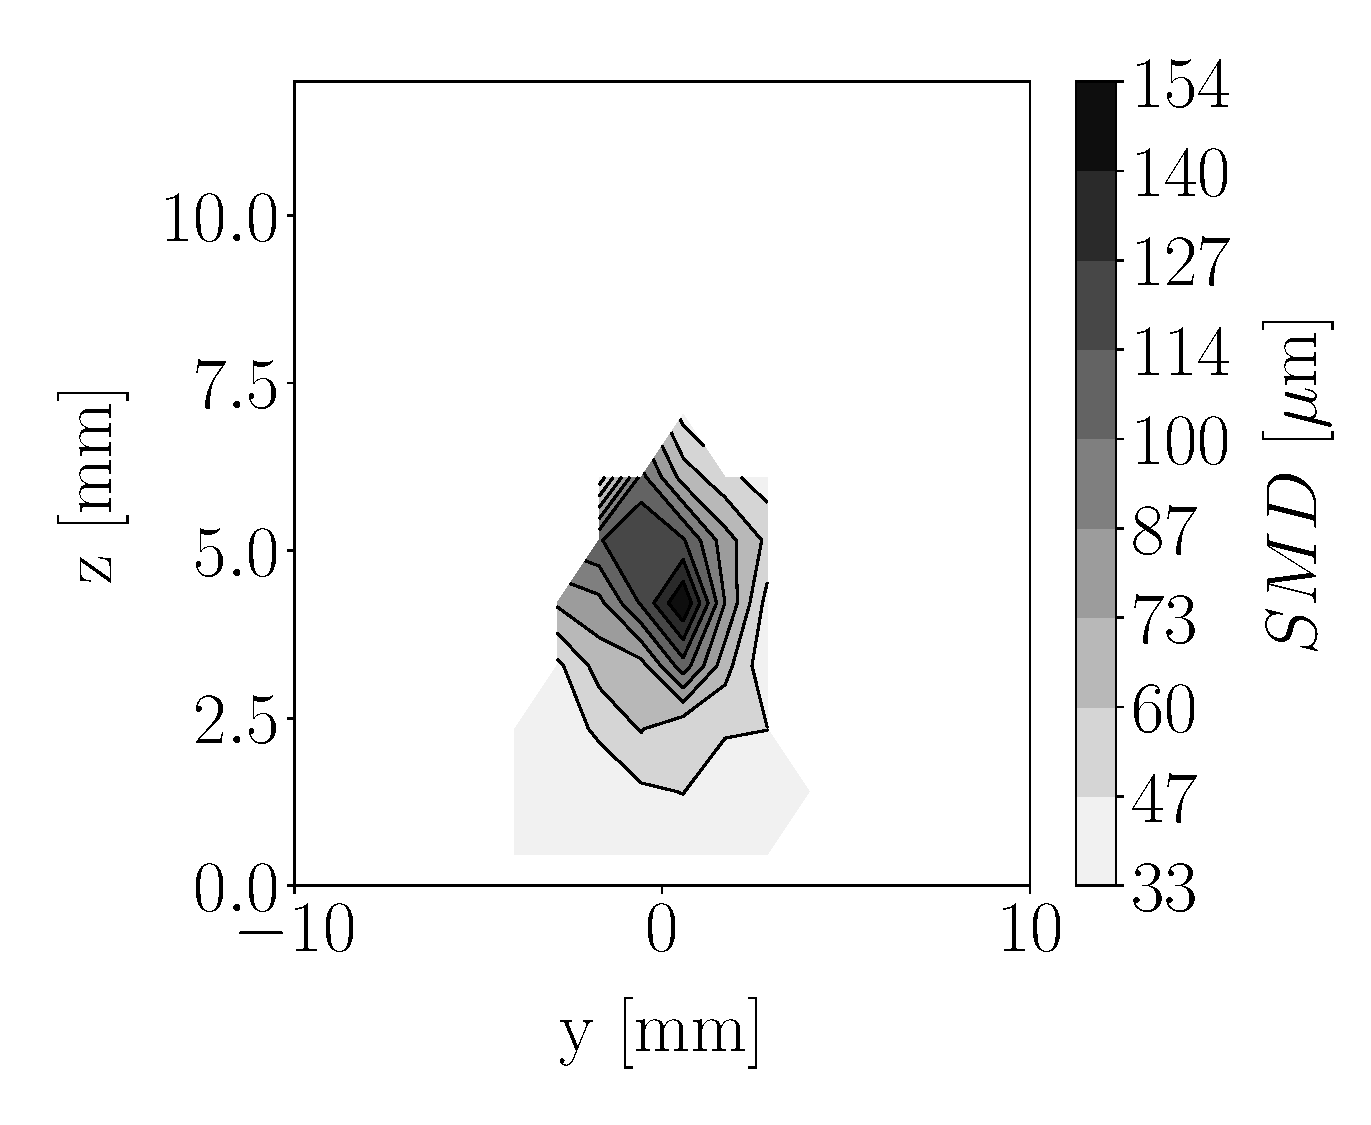
\includegraphics[scale=\scaleSLIJICF]{./part2_developments/figures_ch5_resolved_JICF/injectors_SLI/uG75_dx10_x05_SMD_map}
   %\caption{Case UG100\_DX20: crossflow planes}
   %\label{} 
\end{subfigure}
   \hspace{0.17in}
\begin{subfigure}[b]{0.3\textwidth}
	\centering
   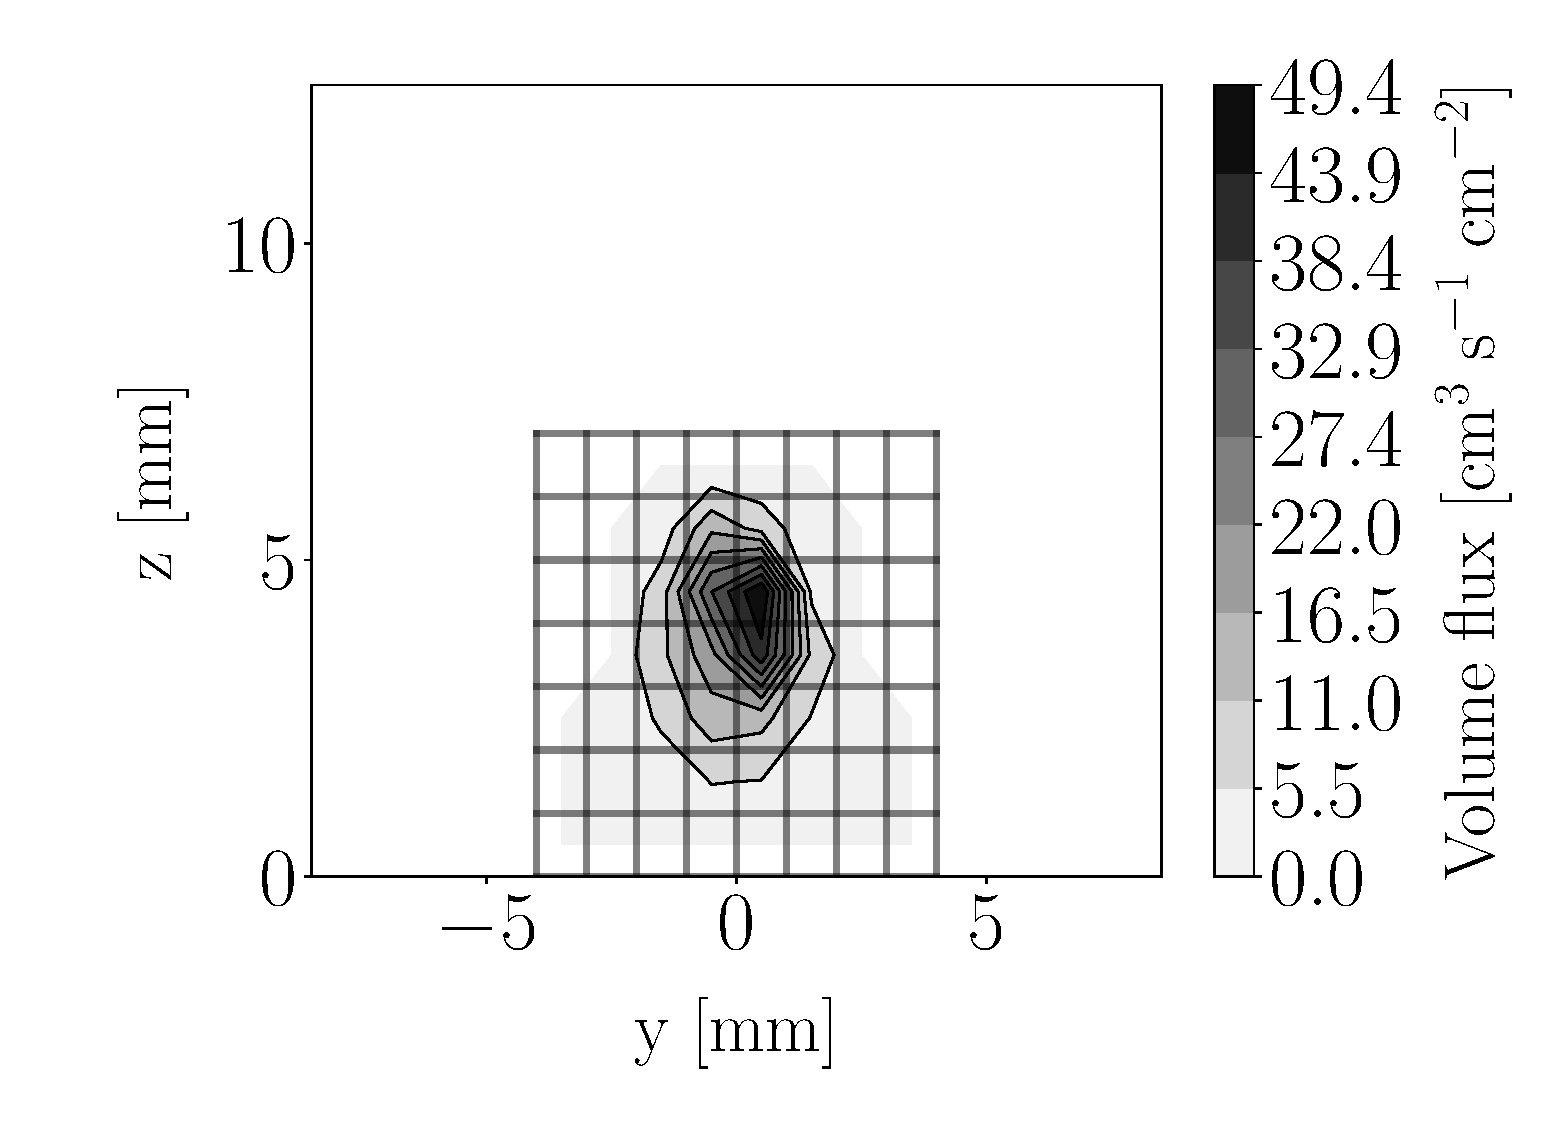
\includegraphics[scale=\scaleSLIJICF]{./part2_developments/figures_ch5_resolved_JICF/injectors_SLI/uG75_dx10_x05_volume_flux_map}
   %\caption{Case UG100\_DX20: filming planes}
   %\label{}
\end{subfigure}
   \hspace{0.17in}
\begin{subfigure}[b]{0.3\textwidth}
	\centering
   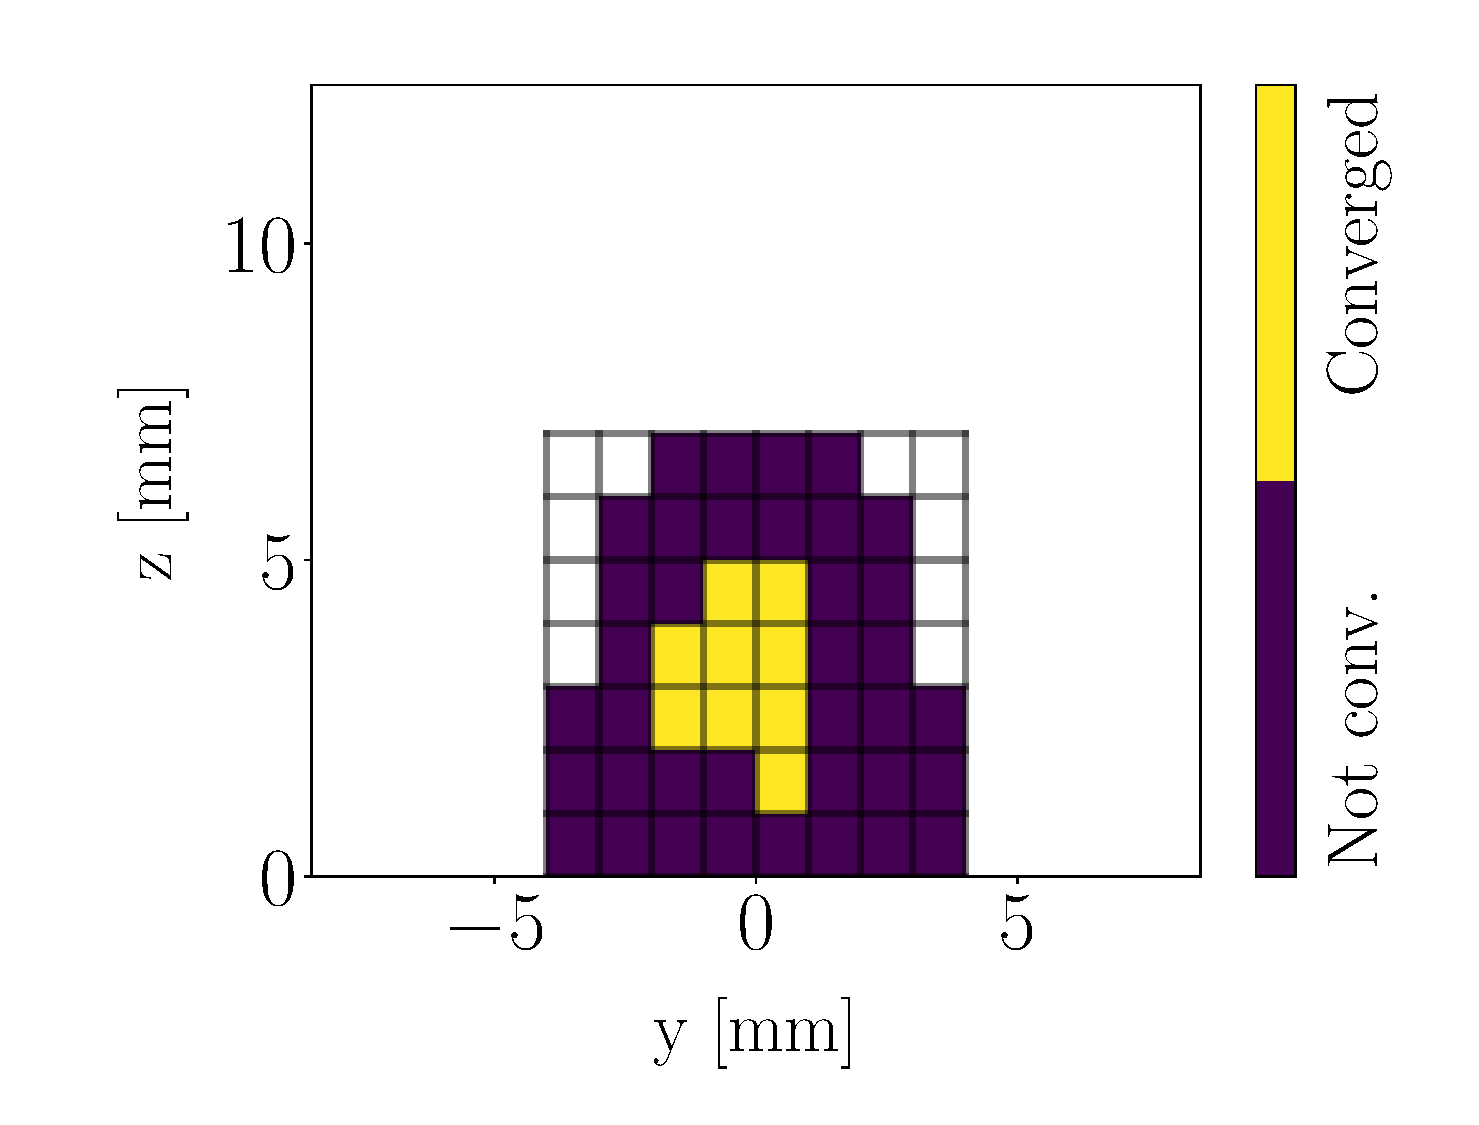
\includegraphics[scale=\scaleSLIJICF]{./part2_developments/figures_ch5_resolved_JICF/injectors_SLI/uG75_dx10_x05_convergence_map}
   %\caption{Case UG100\_DX10: crossflow planes}
   %\label{} 
\end{subfigure}

\vskip\baselineskip

\begin{subfigure}[b]{0.3\textwidth}
	\centering
   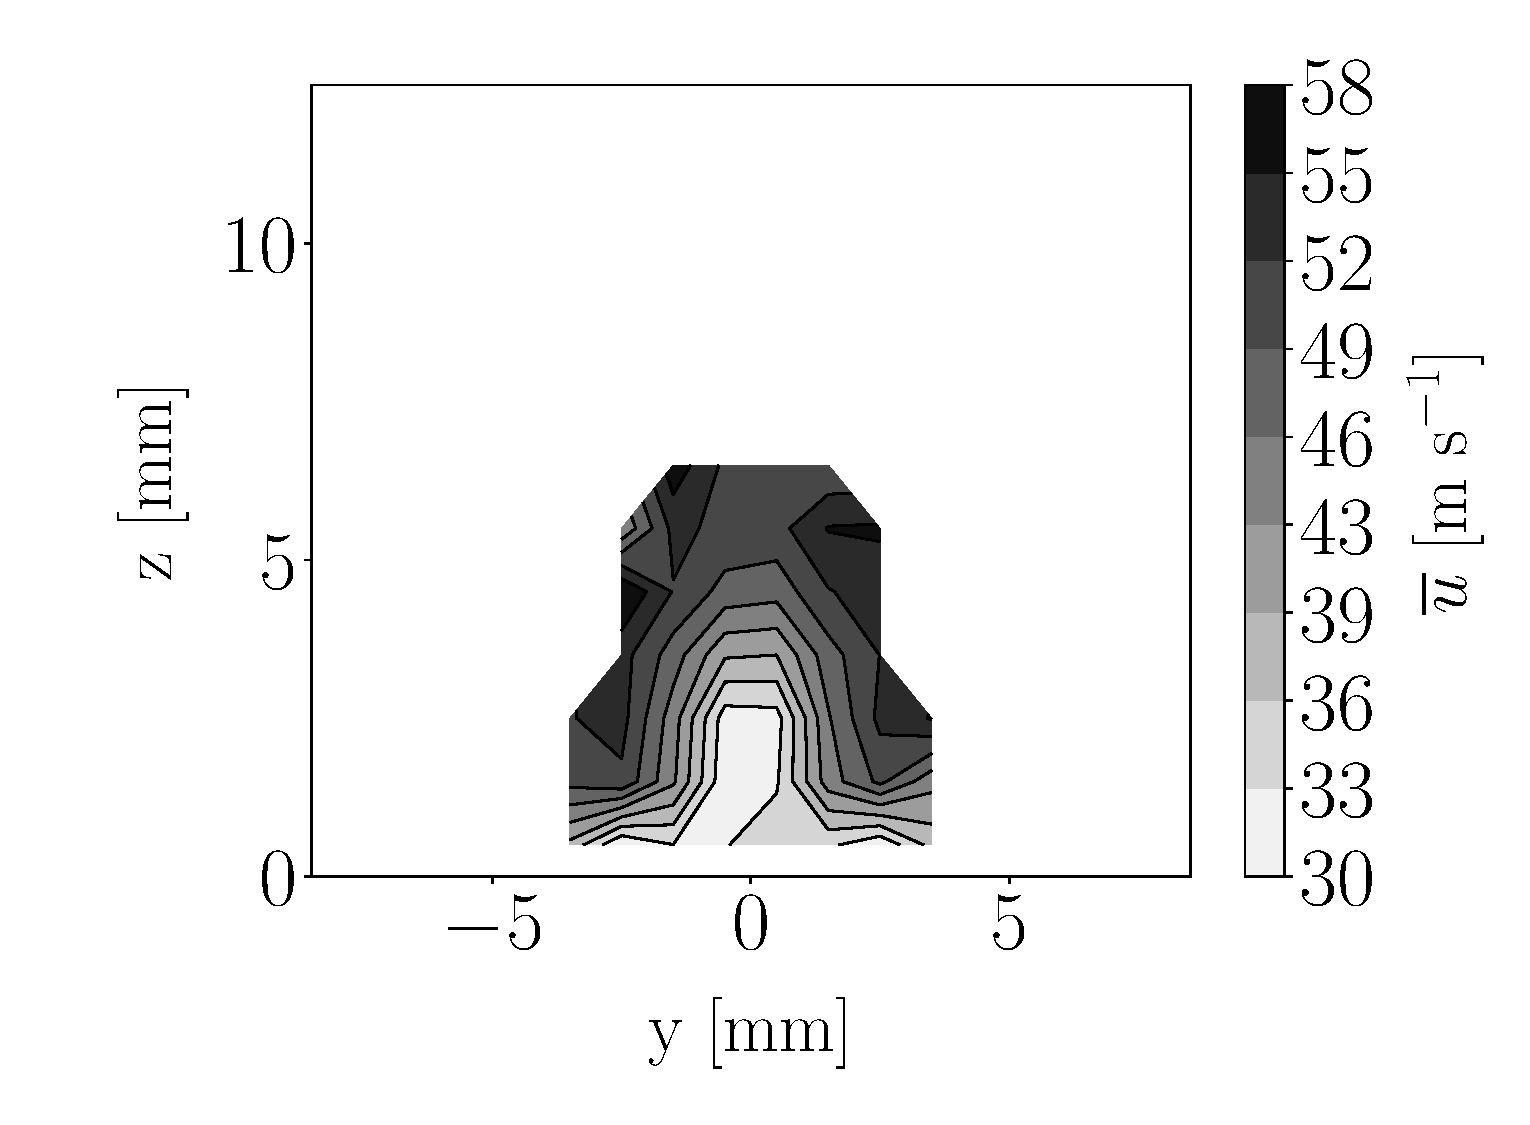
\includegraphics[scale=\scaleSLIJICF]{./part2_developments/figures_ch5_resolved_JICF/injectors_SLI/uG75_dx10_x05_ux_mean_map}
   %\caption{Case UG100\_DX20: crossflow planes}
   %\label{} 
\end{subfigure}
   \hspace{0.17in}
\begin{subfigure}[b]{0.3\textwidth}
	\centering
   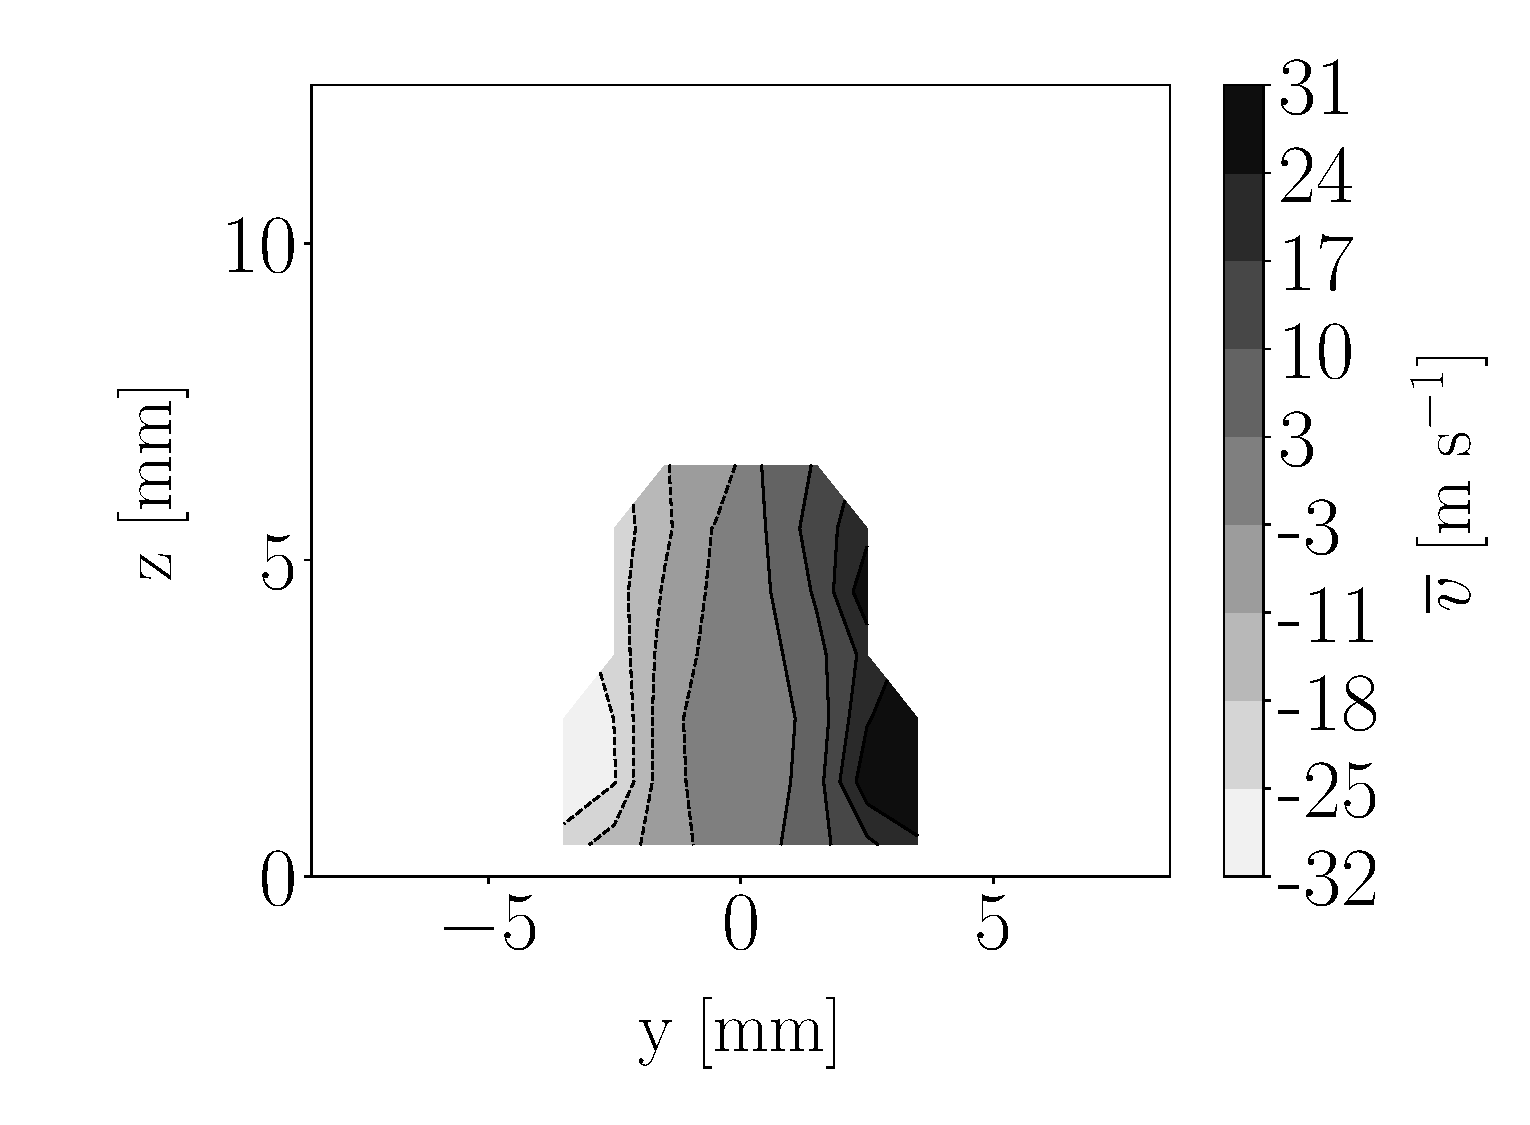
\includegraphics[scale=\scaleSLIJICF]{./part2_developments/figures_ch5_resolved_JICF/injectors_SLI/uG75_dx10_x05_uy_mean_map}
   %\caption{Case UG100\_DX20: filming planes}
   %\label{}
\end{subfigure}
   \hspace{0.17in}
\begin{subfigure}[b]{0.3\textwidth}
	\centering
   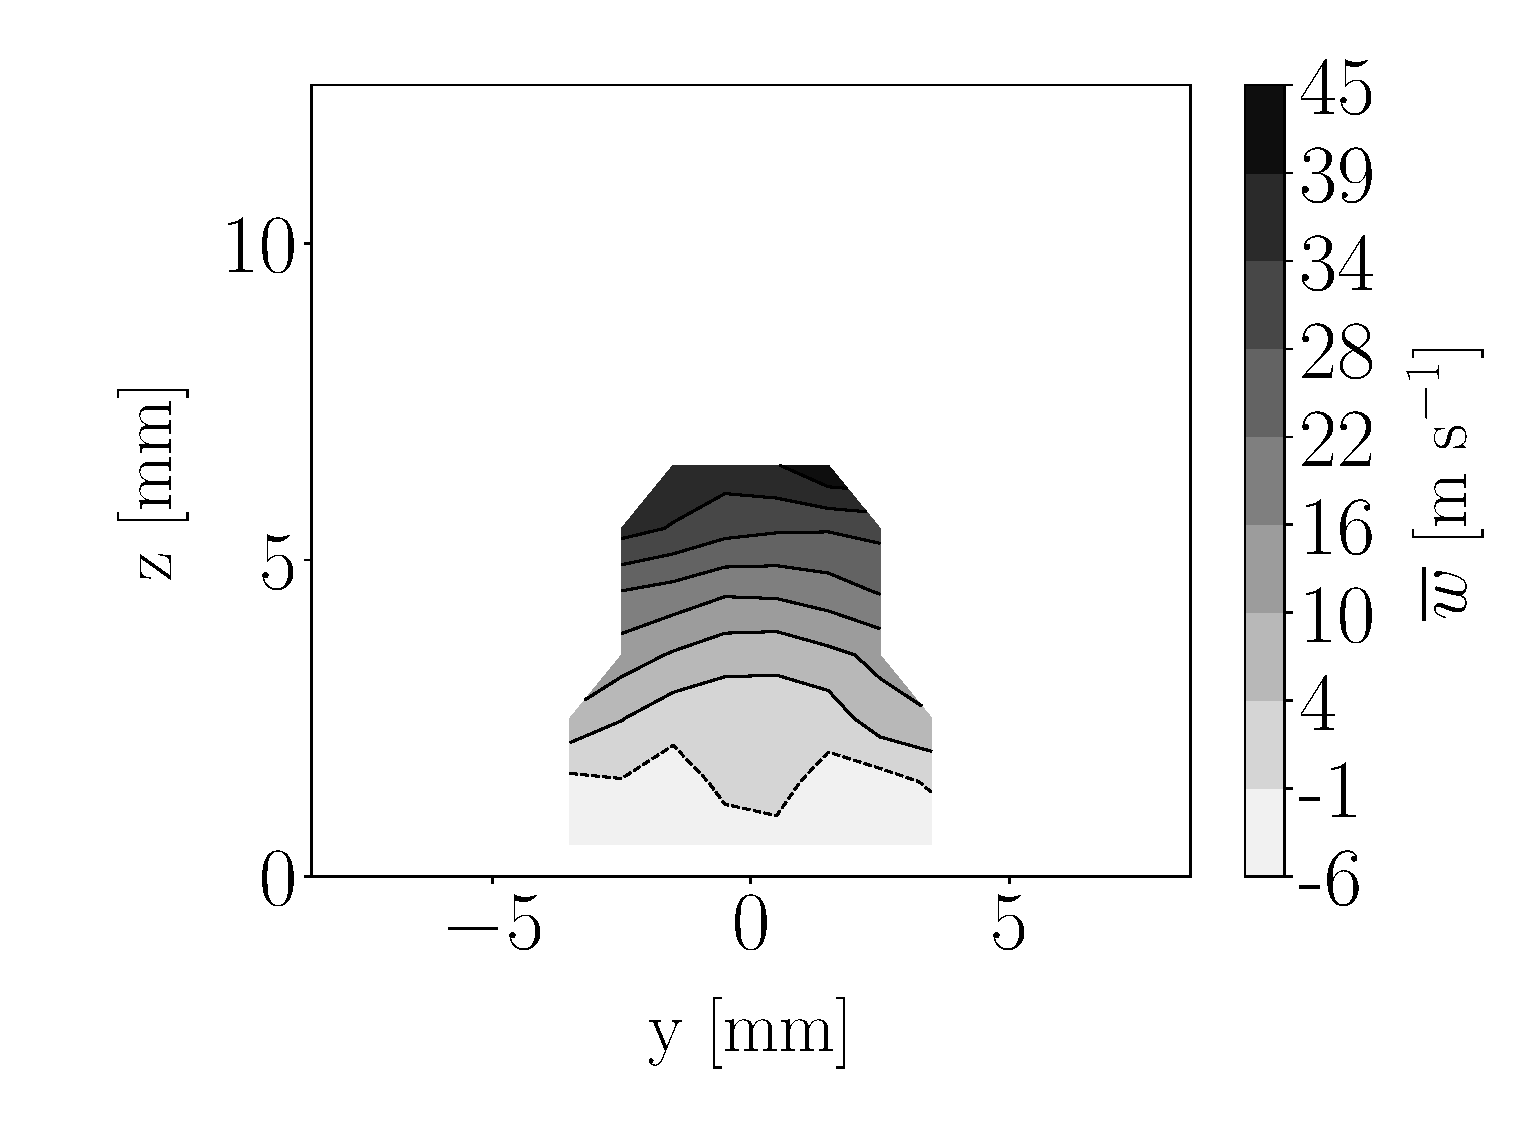
\includegraphics[scale=\scaleSLIJICF]{./part2_developments/figures_ch5_resolved_JICF/injectors_SLI/uG75_dx10_x05_uz_mean_map}
   %\caption{Case UG100\_DX10: crossflow planes}
   %\label{} 
\end{subfigure}
\caption{Spray states at x = 5 mm for case UG75\_DX10}
\label{fig:injectors_sli_uG75_dx10_x05}
\end{figure}


%%%%%%%%%%%%%%%% UG75_DX10, x = 10 mm


\begin{figure}[h!]
\centering
\begin{subfigure}[b]{0.3\textwidth}
	\centering
   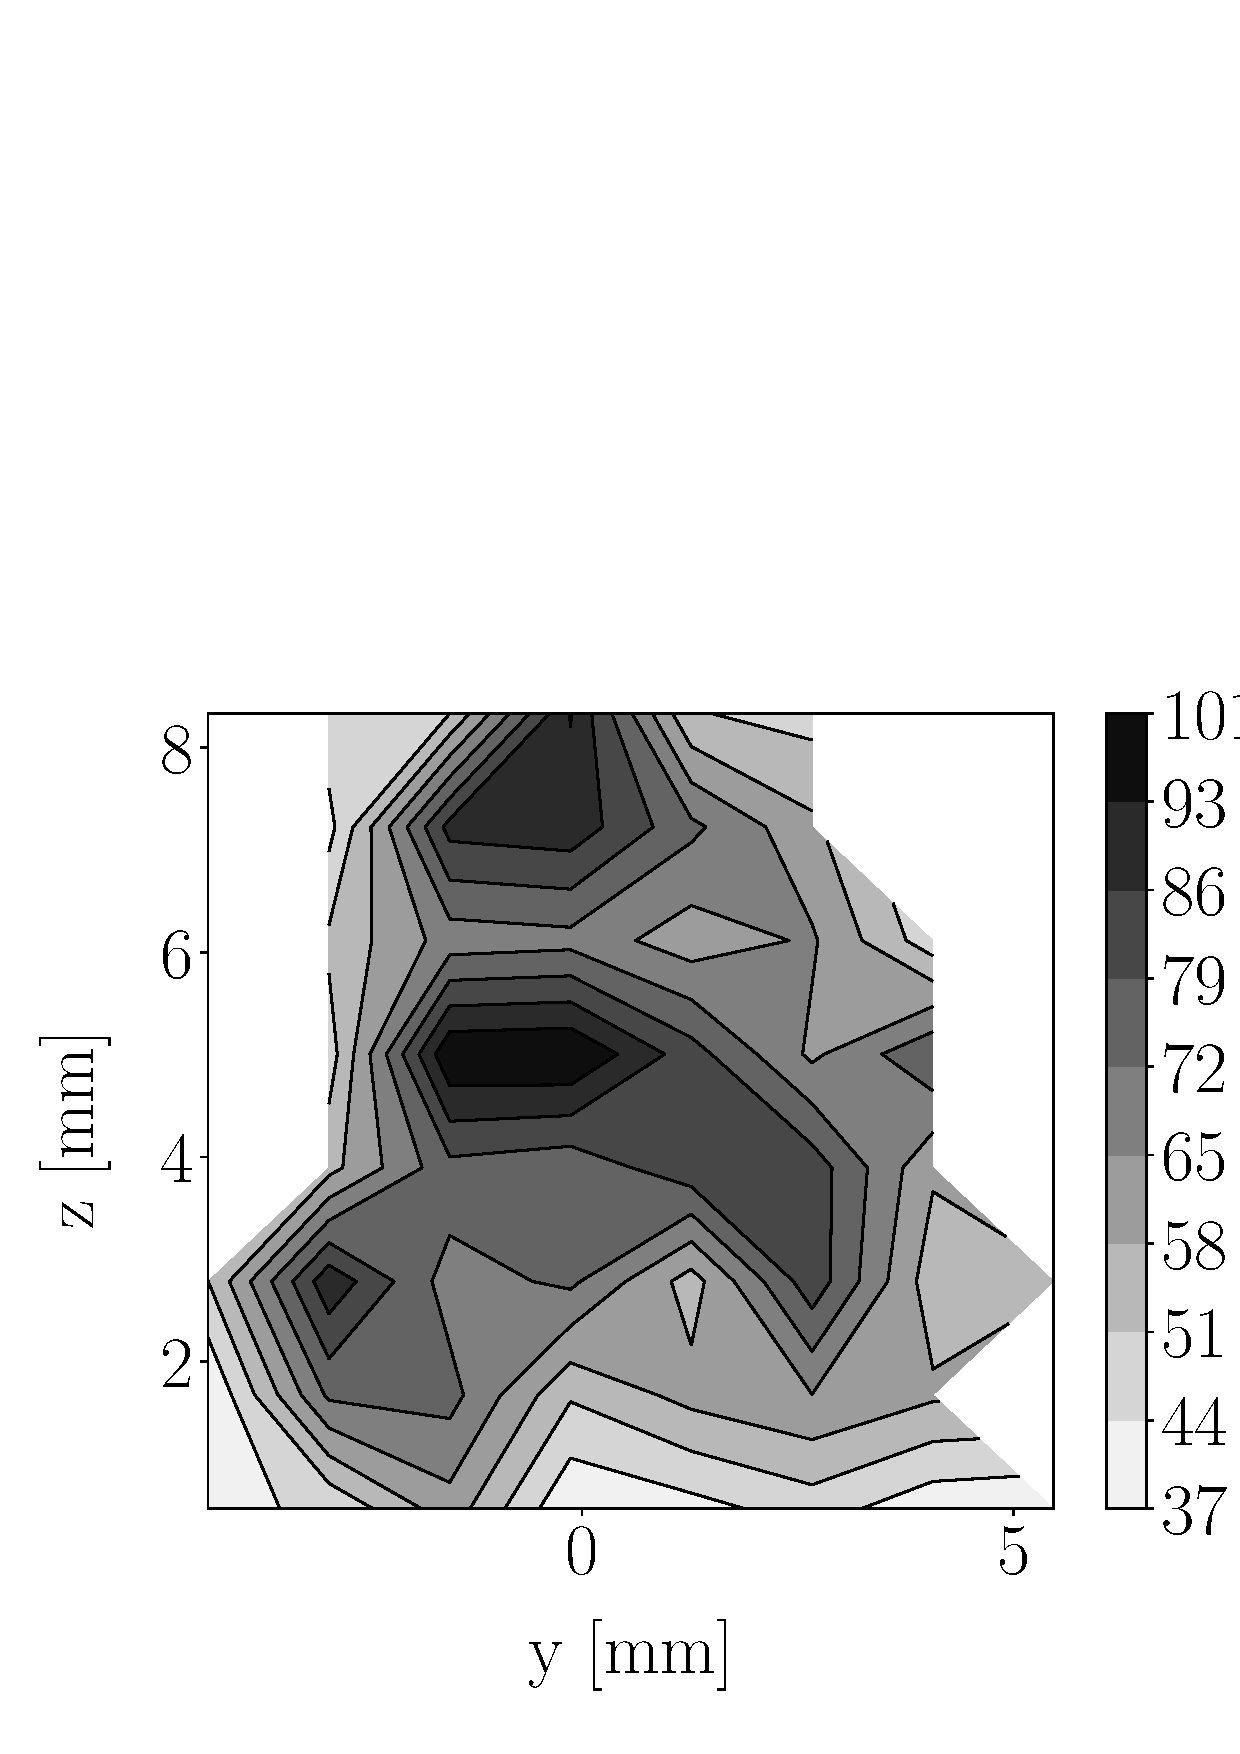
\includegraphics[scale=\scaleSLIJICF]{./part2_developments/figures_ch5_resolved_JICF/injectors_SLI/uG75_dx10_x10_SMD_map}
   %\caption{Case UG100\_DX20: crossflow planes}
   %\label{} 
\end{subfigure}
   \hspace{0.17in}
\begin{subfigure}[b]{0.3\textwidth}
	\centering
   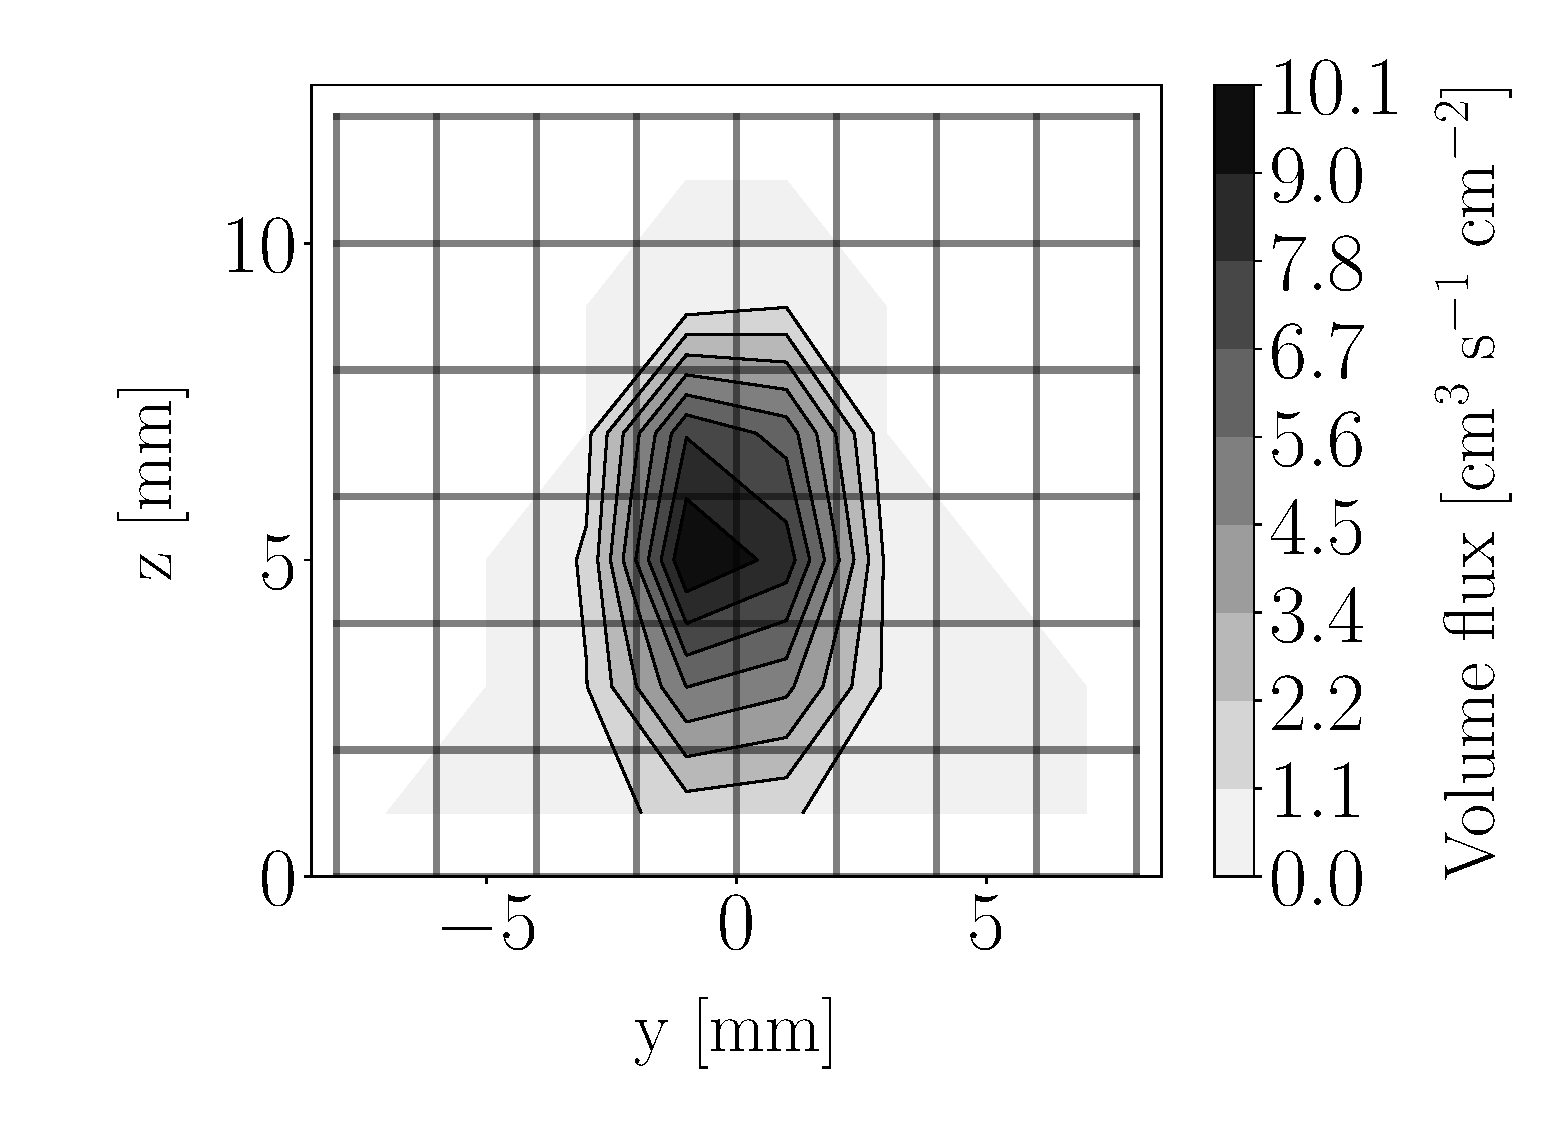
\includegraphics[scale=\scaleSLIJICF]{./part2_developments/figures_ch5_resolved_JICF/injectors_SLI/uG75_dx10_x10_volume_flux_map}
   %\caption{Case UG100\_DX20: filming planes}
   %\label{}
\end{subfigure}
   \hspace{0.17in}
\begin{subfigure}[b]{0.3\textwidth}
	\centering
   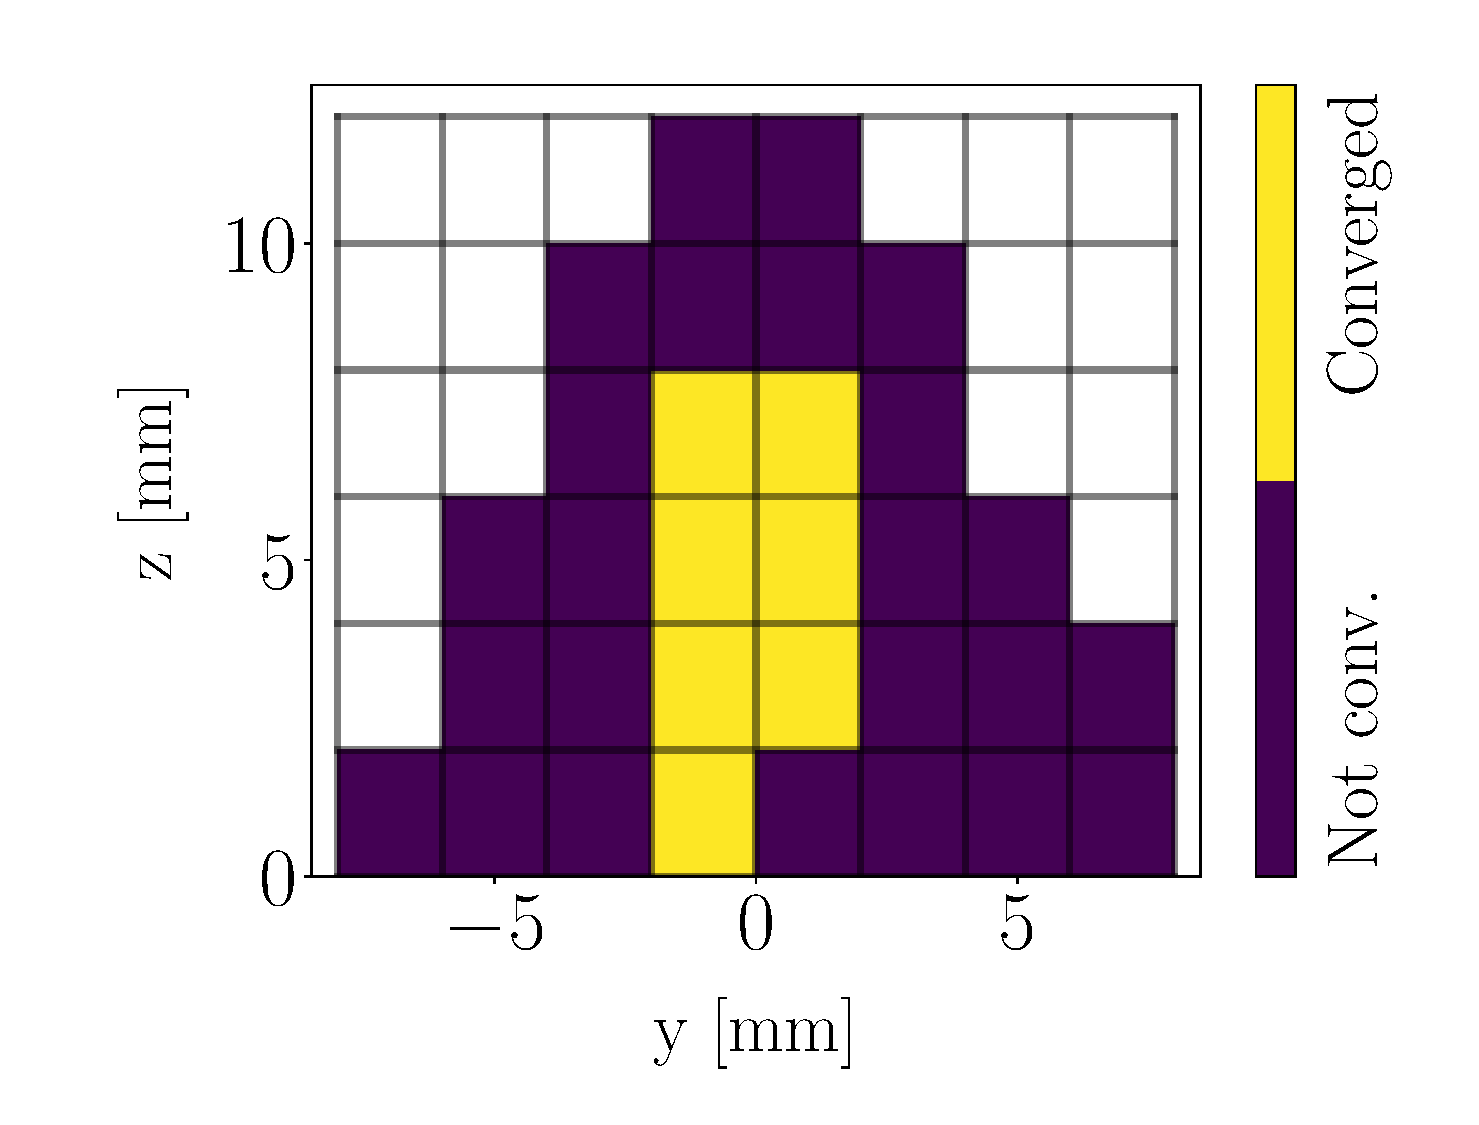
\includegraphics[scale=\scaleSLIJICF]{./part2_developments/figures_ch5_resolved_JICF/injectors_SLI/uG75_dx10_x10_convergence_map}
   %\caption{Case UG100\_DX10: crossflow planes}
   %\label{} 
\end{subfigure}

\vskip\baselineskip

\begin{subfigure}[b]{0.3\textwidth}
	\centering
   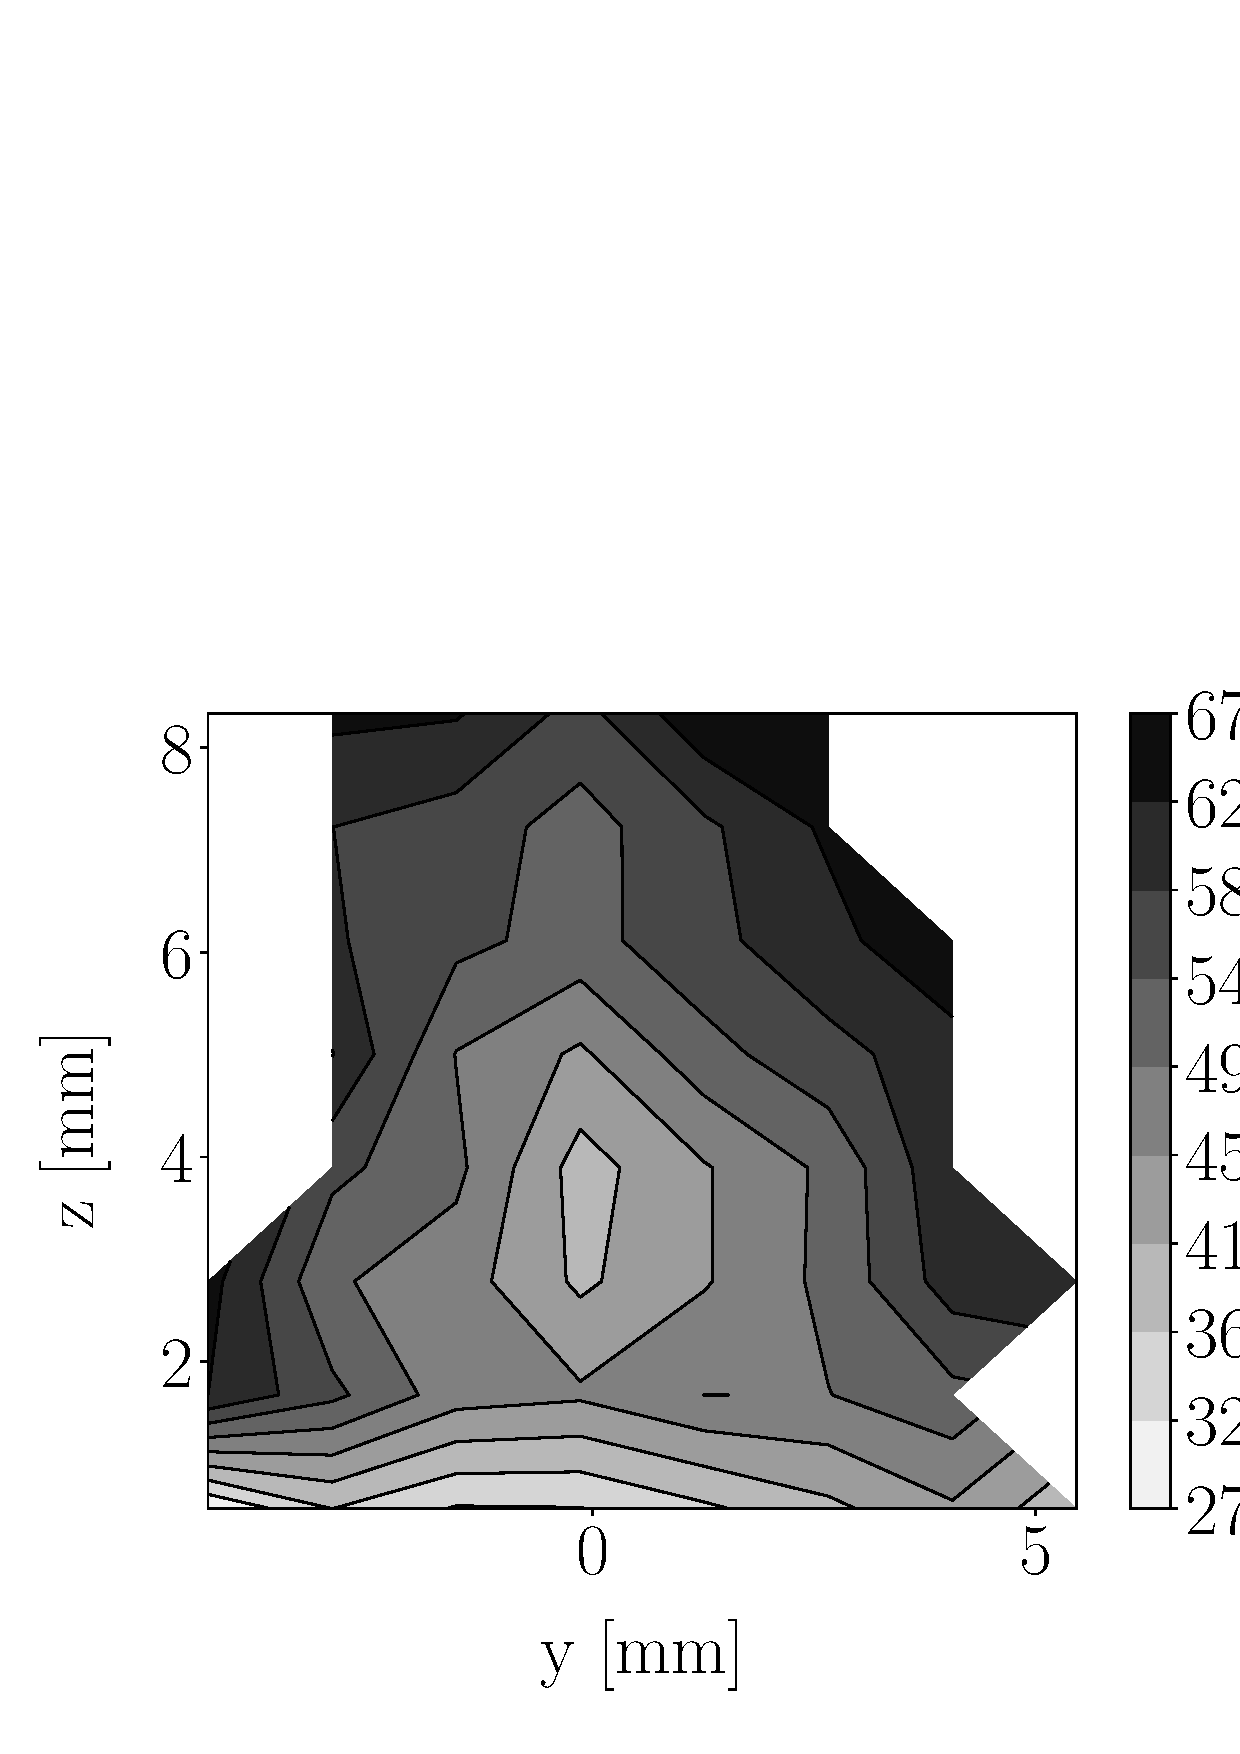
\includegraphics[scale=\scaleSLIJICF]{./part2_developments/figures_ch5_resolved_JICF/injectors_SLI/uG75_dx10_x10_ux_mean_map}
   %\caption{Case UG100\_DX20: crossflow planes}
   %\label{} 
\end{subfigure}
   \hspace{0.17in}
\begin{subfigure}[b]{0.3\textwidth}
	\centering
   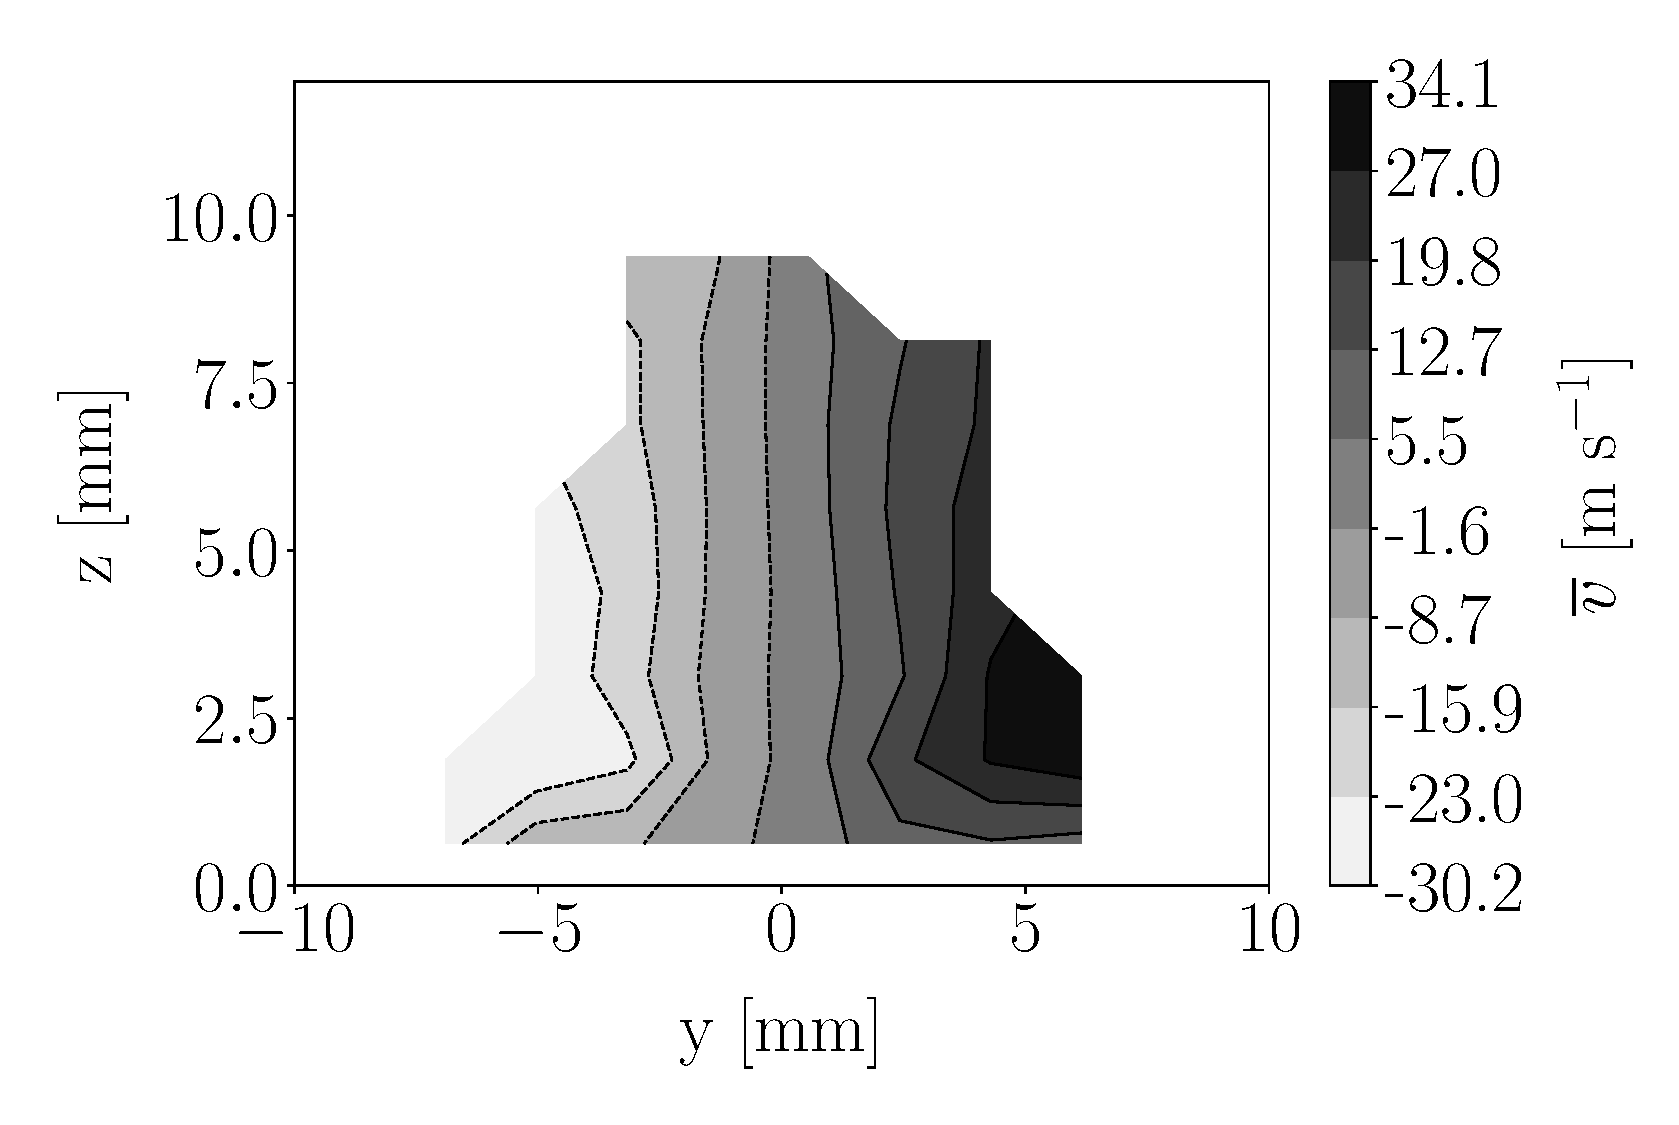
\includegraphics[scale=\scaleSLIJICF]{./part2_developments/figures_ch5_resolved_JICF/injectors_SLI/uG75_dx10_x10_uy_mean_map}
   %\caption{Case UG100\_DX20: filming planes}
   %\label{}
\end{subfigure}
   \hspace{0.17in}
\begin{subfigure}[b]{0.3\textwidth}
	\centering
   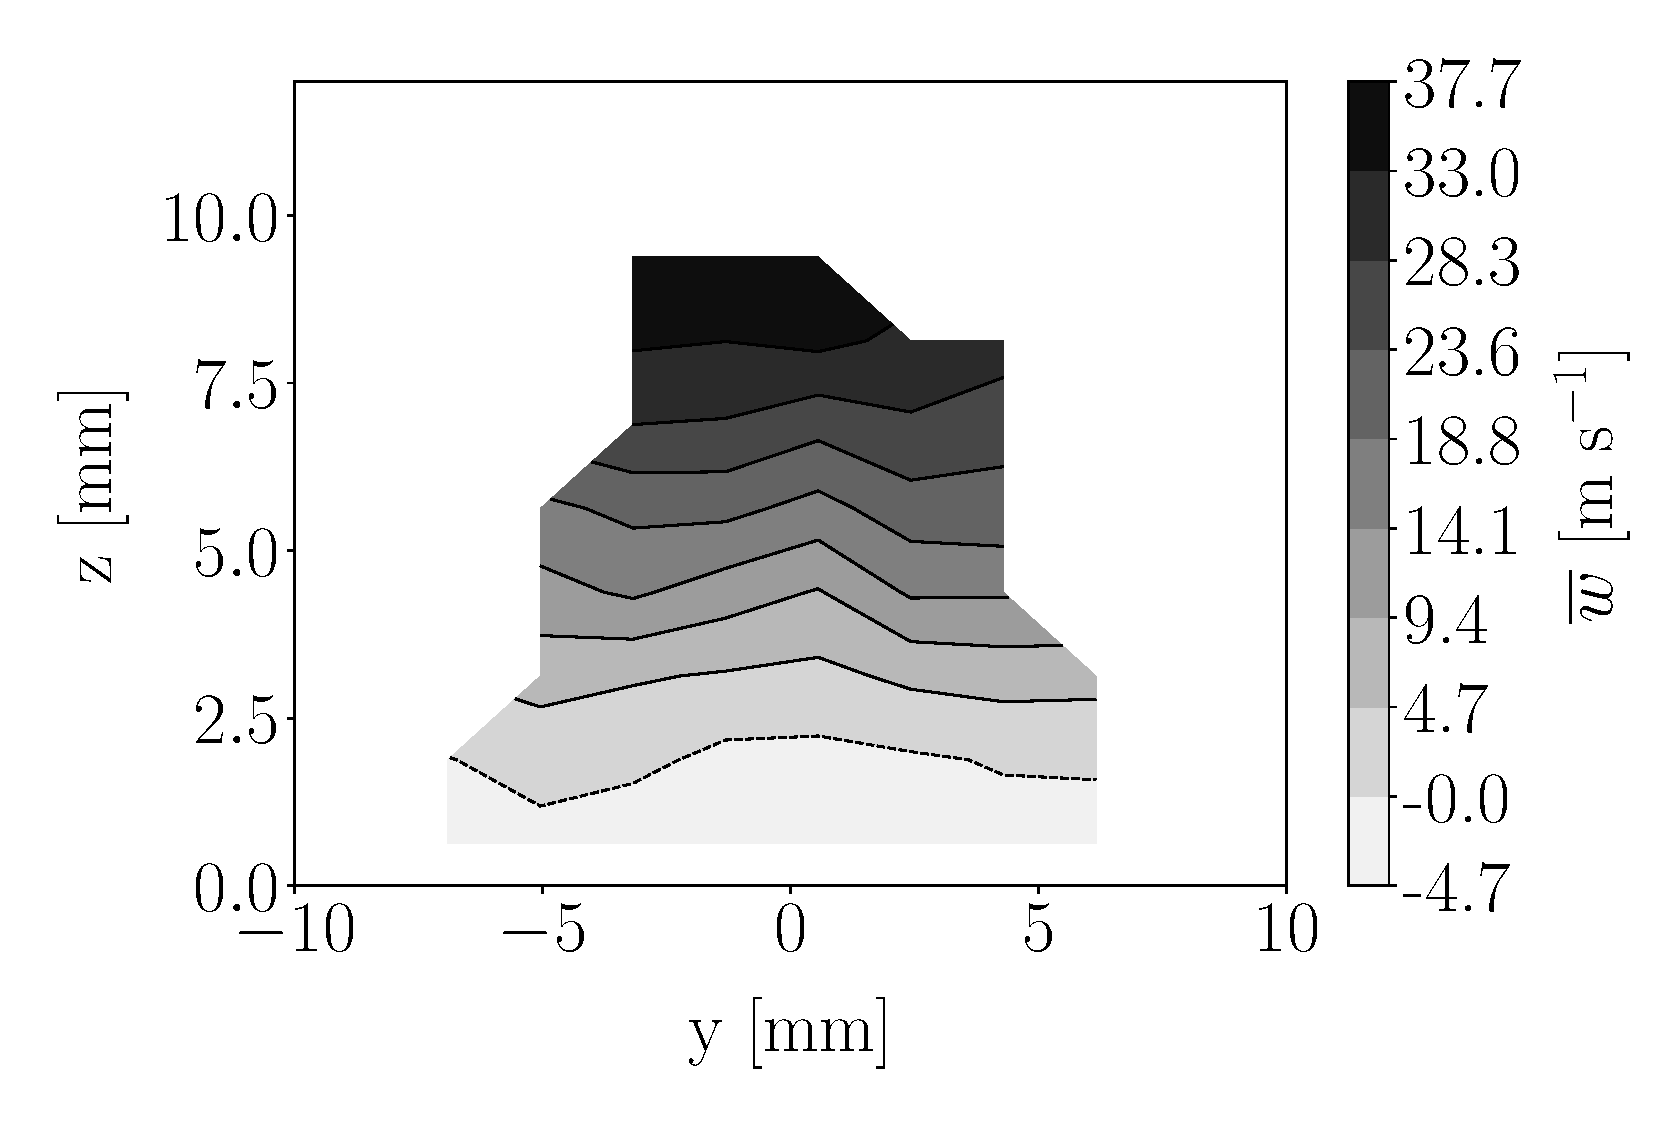
\includegraphics[scale=\scaleSLIJICF]{./part2_developments/figures_ch5_resolved_JICF/injectors_SLI/uG75_dx10_x10_uz_mean_map}
   %\caption{Case UG100\_DX10: crossflow planes}
   %\label{} 
\end{subfigure}
\caption{Spray states at x = 10 mm for case UG75\_DX10}
\label{fig:injectors_sli_uG75_dx10_x10}
\end{figure}


\clearpage

\subsubsection*{Case UG75\_DX20}


%%%%%%%%%%%%%%%% UG75_DX20, x = 5 mm


\begin{figure}[h!]
\centering
\begin{subfigure}[b]{0.3\textwidth}
	\centering
   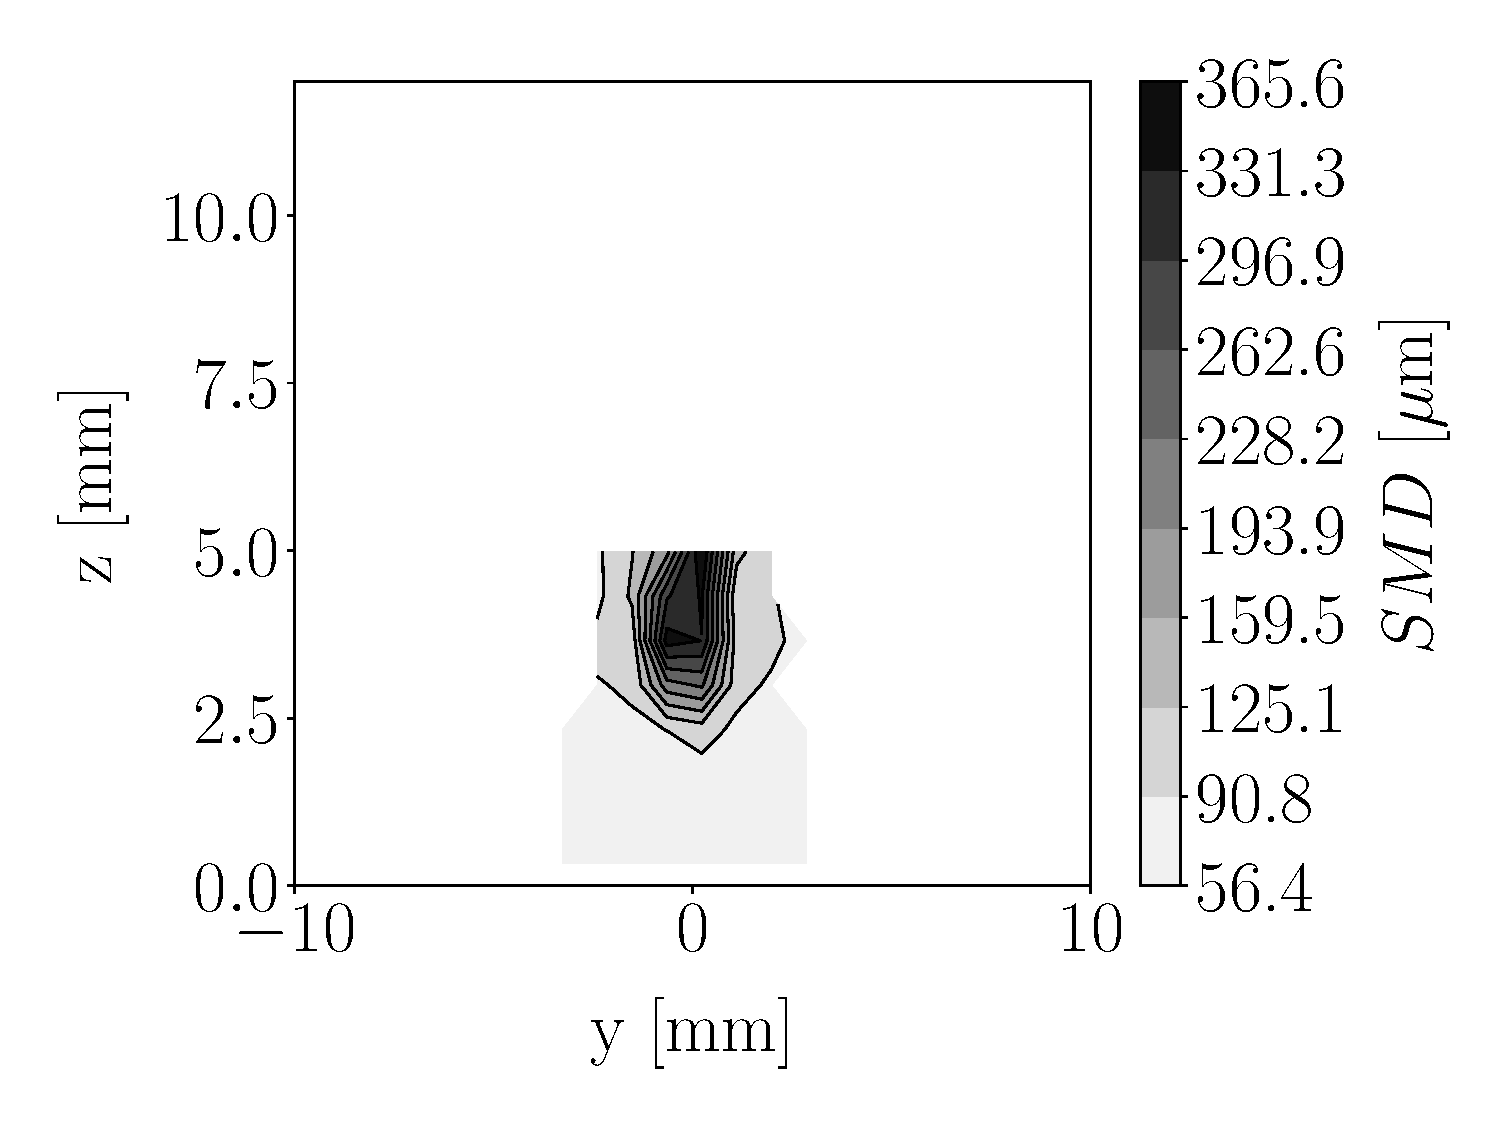
\includegraphics[scale=\scaleSLIJICF]{./part2_developments/figures_ch5_resolved_JICF/injectors_SLI/uG75_dx20_x05_SMD_map}
   %\caption{Case UG100\_DX20: crossflow planes}
   %\label{} 
\end{subfigure}
   \hspace{0.17in}
\begin{subfigure}[b]{0.3\textwidth}
	\centering
   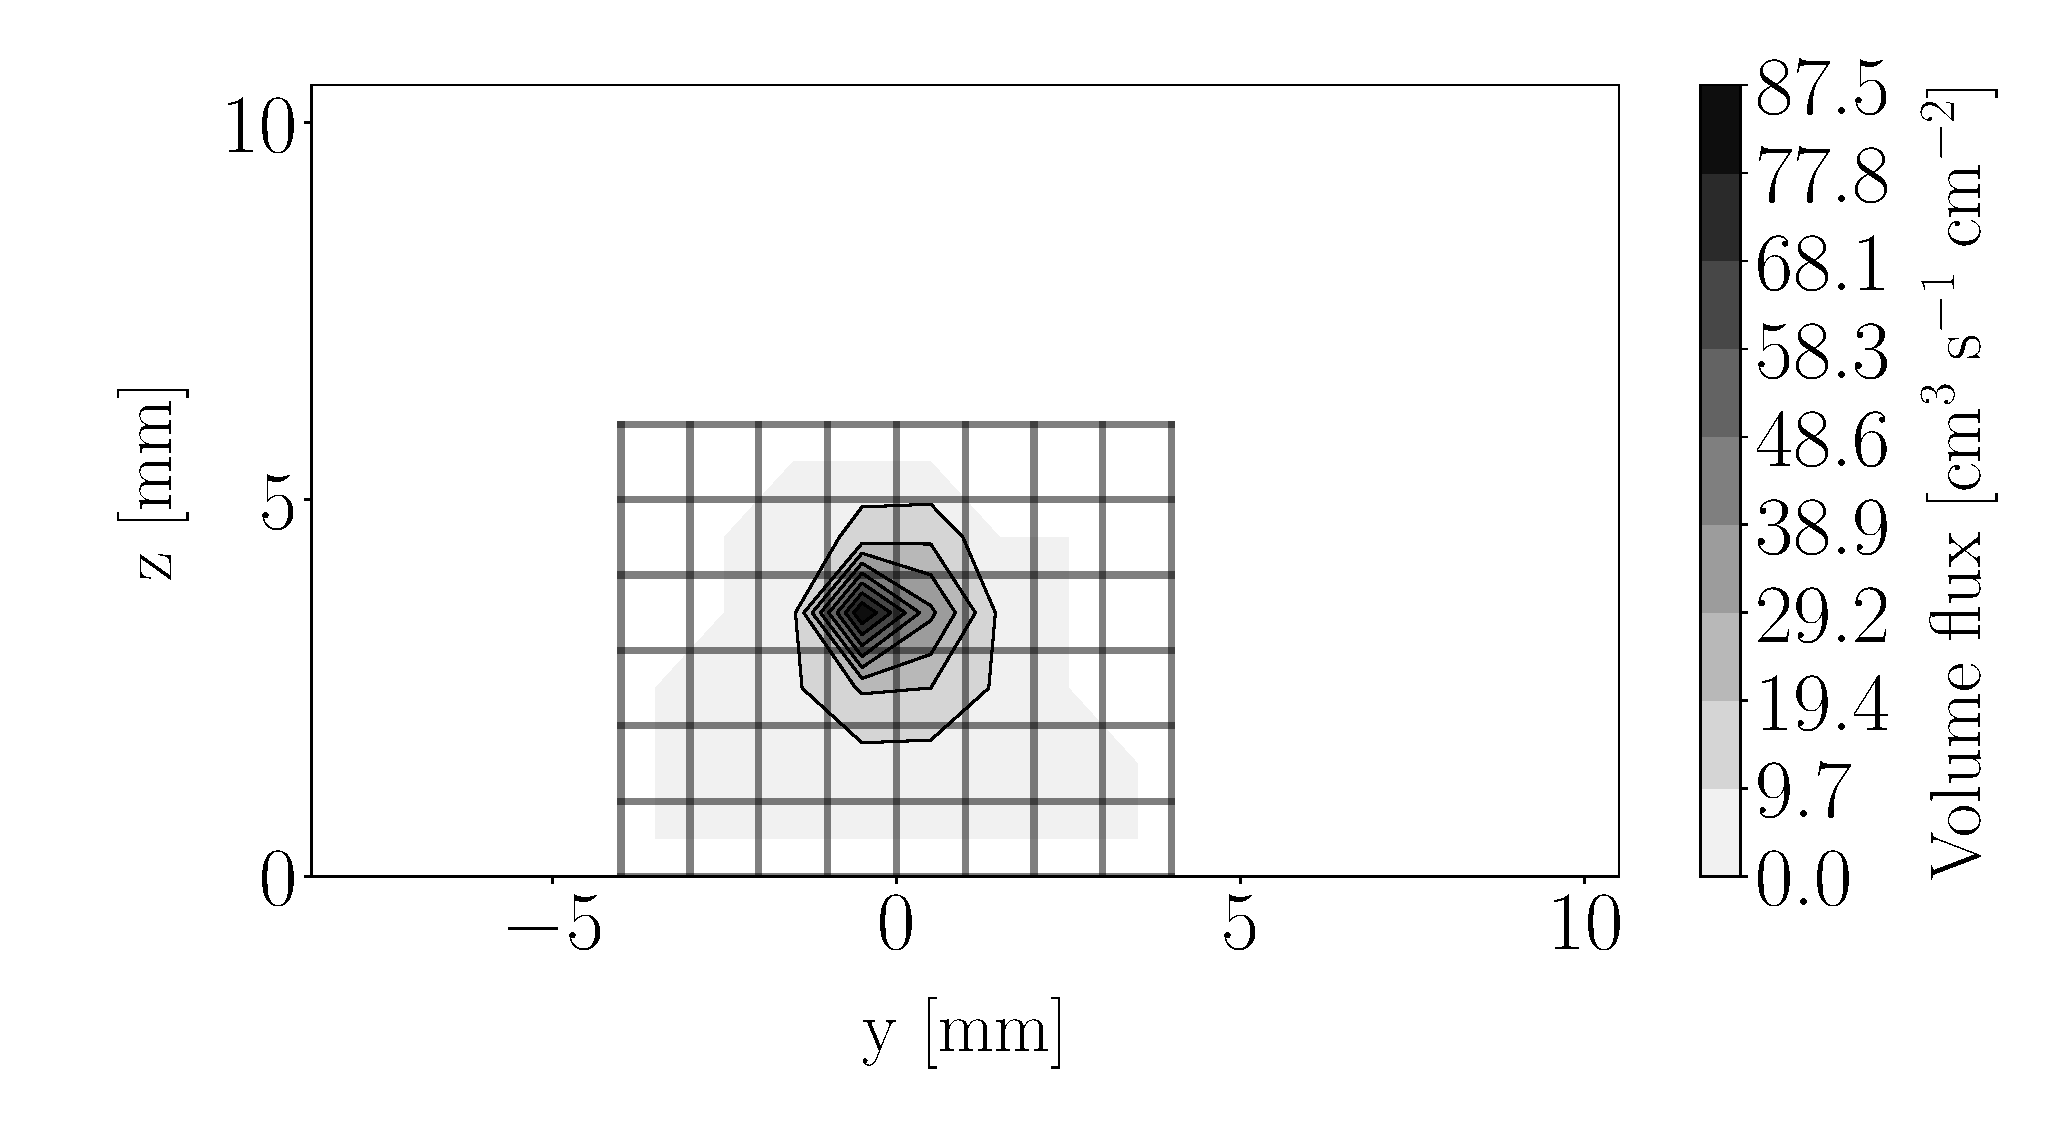
\includegraphics[scale=\scaleSLIJICF]{./part2_developments/figures_ch5_resolved_JICF/injectors_SLI/uG75_dx20_x05_volume_flux_map}
   %\caption{Case UG100\_DX20: filming planes}
   %\label{}
\end{subfigure}
   \hspace{0.17in}
\begin{subfigure}[b]{0.3\textwidth}
	\centering
   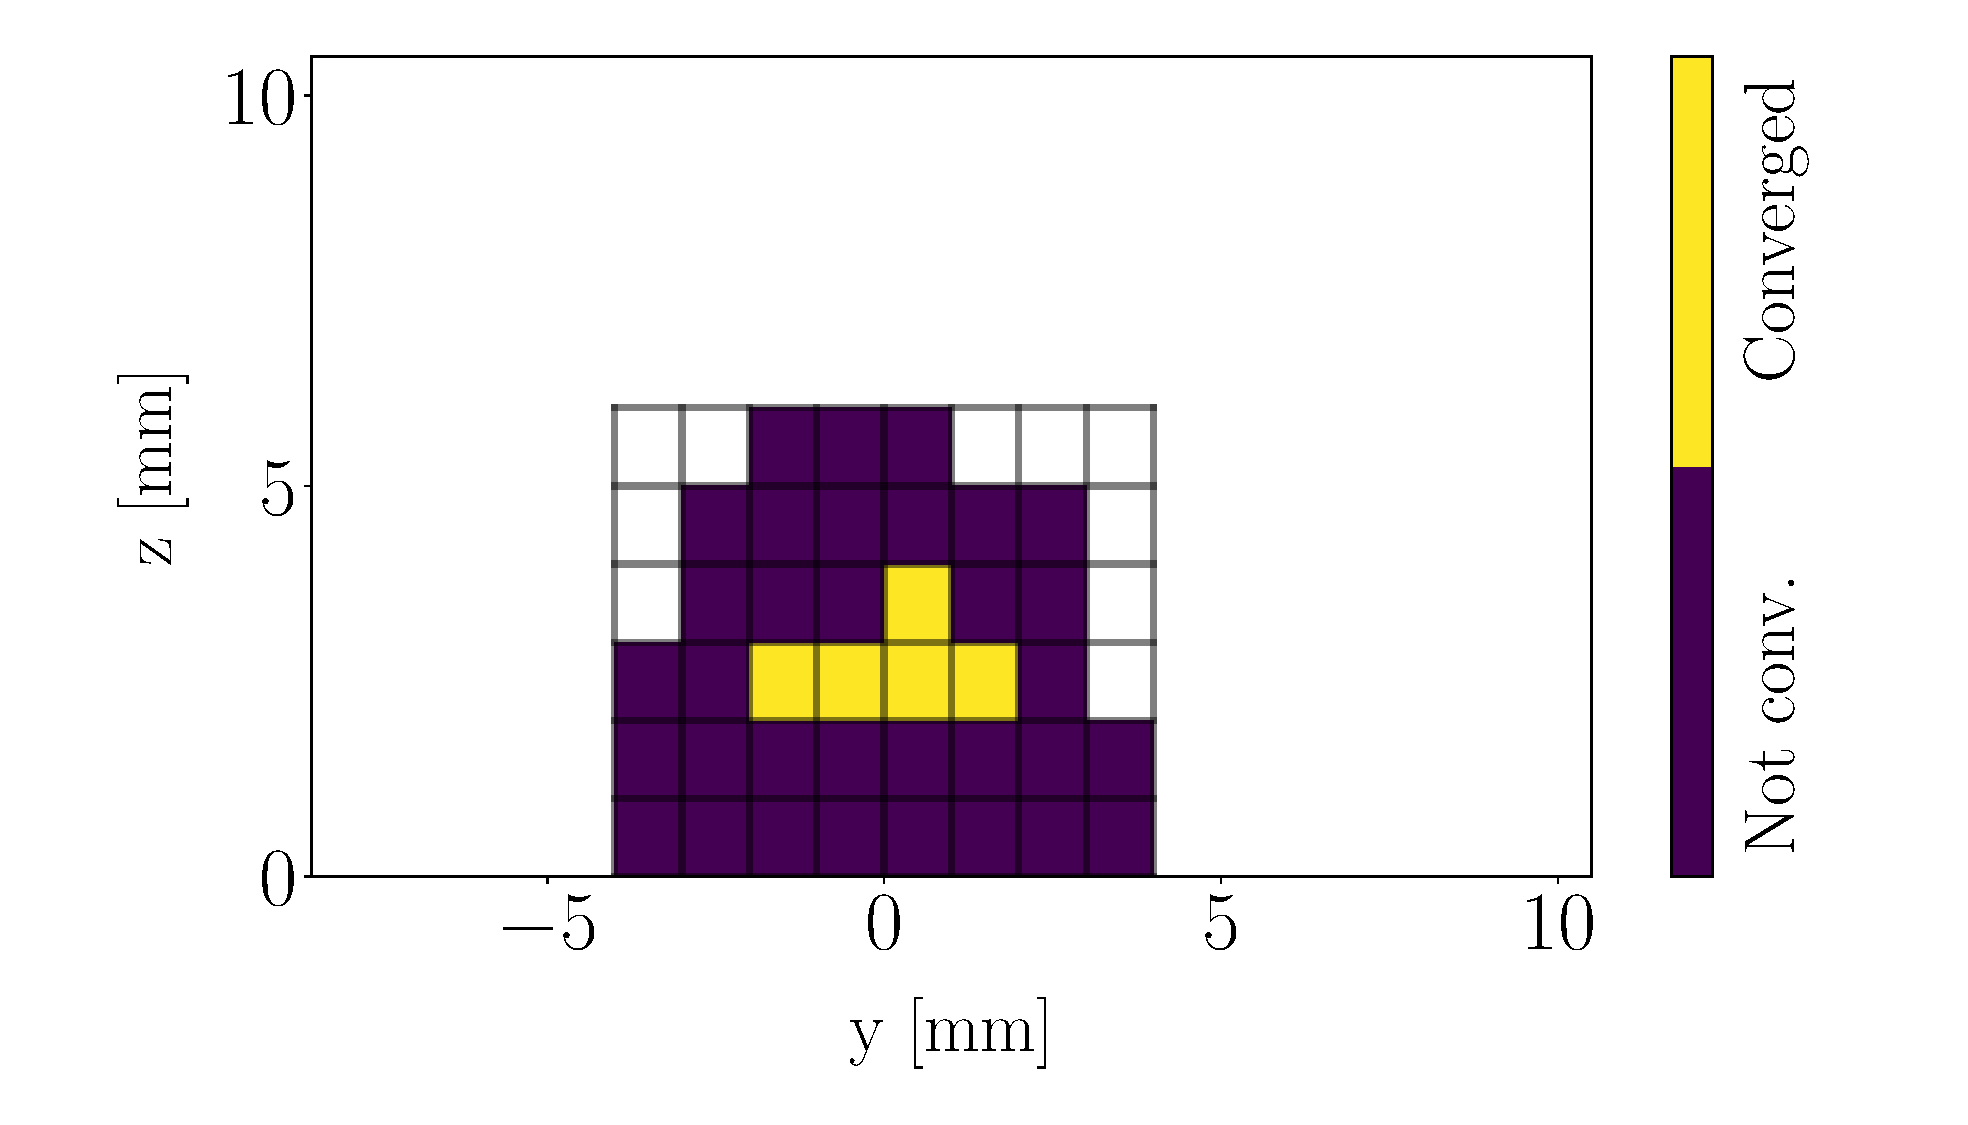
\includegraphics[scale=\scaleSLIJICF]{./part2_developments/figures_ch5_resolved_JICF/injectors_SLI/uG75_dx20_x05_convergence_map}
   %\caption{Case UG100\_DX10: crossflow planes}
   %\label{} 
\end{subfigure}

\vskip\baselineskip

\begin{subfigure}[b]{0.3\textwidth}
	\centering
   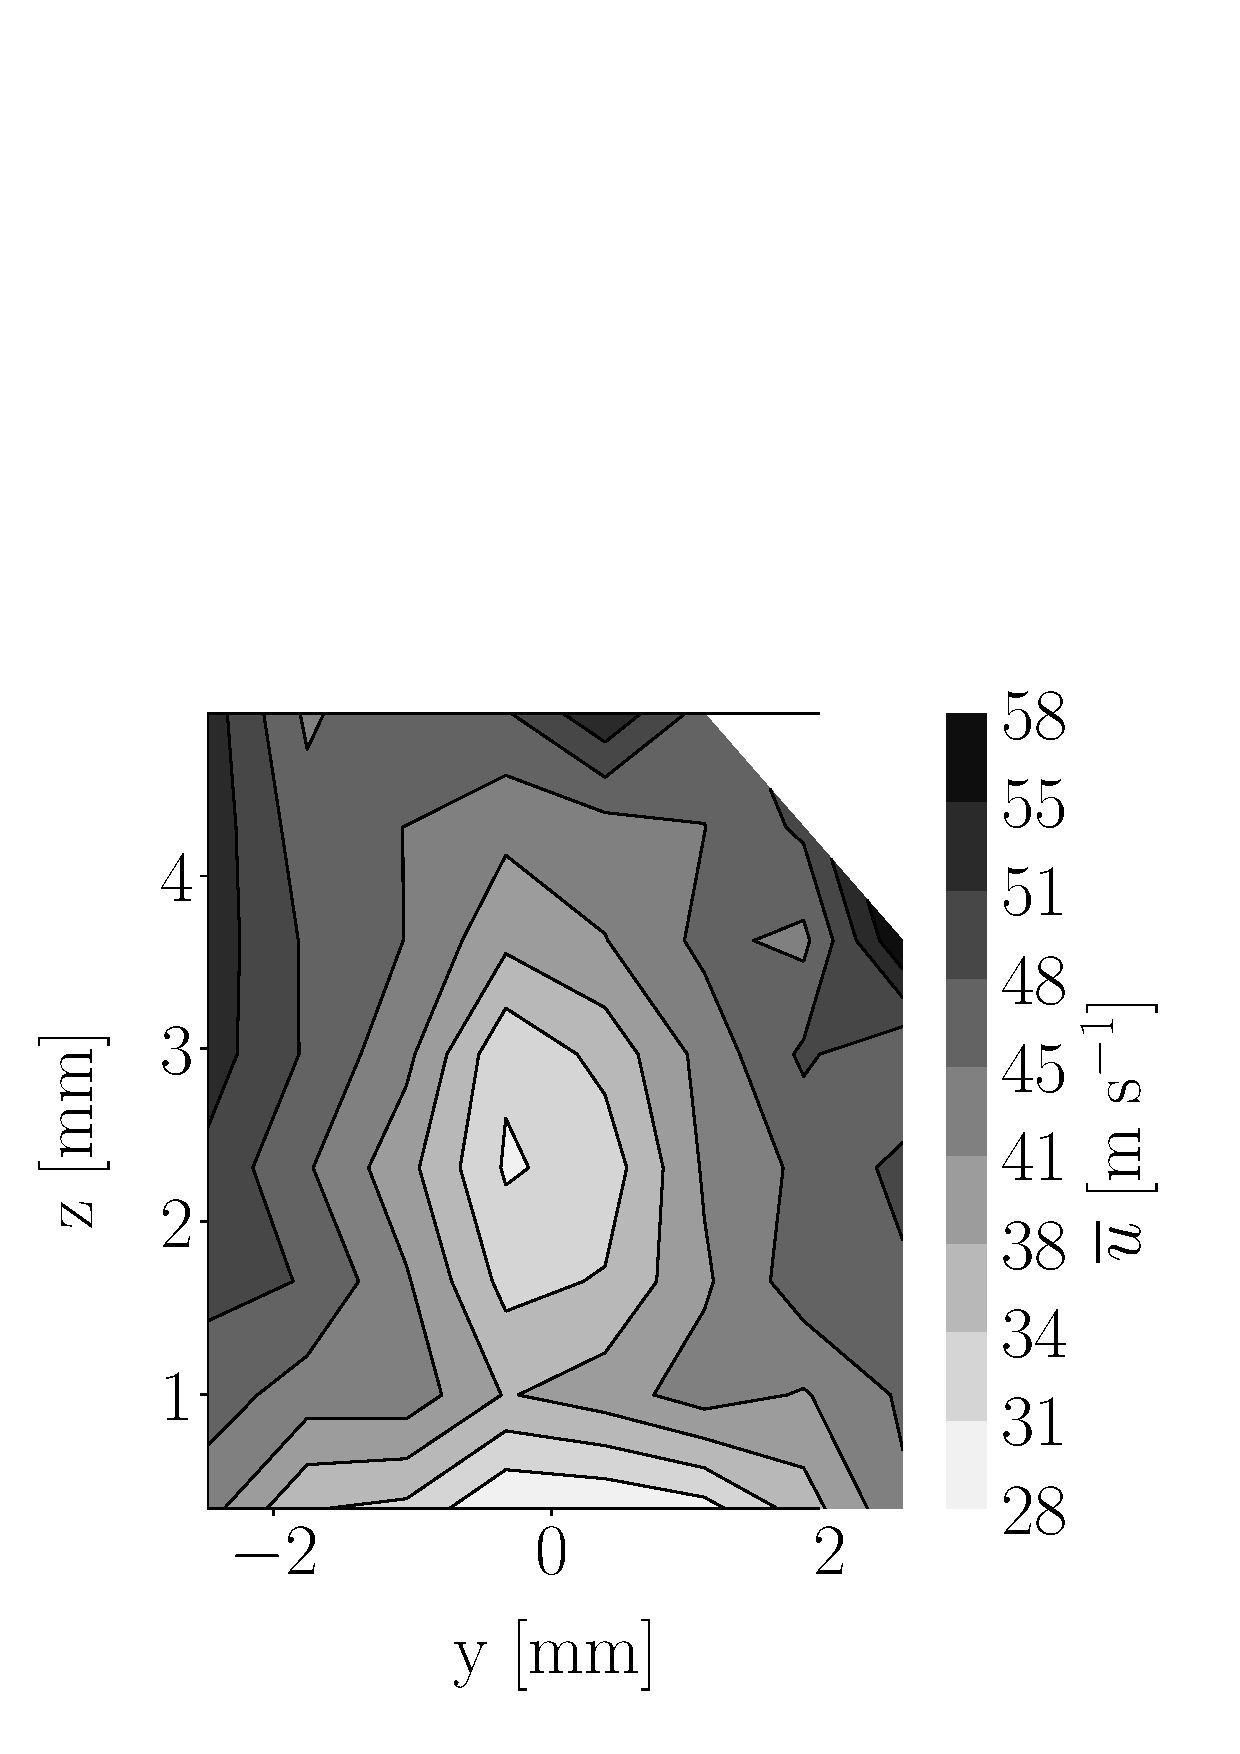
\includegraphics[scale=\scaleSLIJICF]{./part2_developments/figures_ch5_resolved_JICF/injectors_SLI/uG75_dx20_x05_ux_mean_map}
   %\caption{Case UG100\_DX20: crossflow planes}
   %\label{} 
\end{subfigure}
   \hspace{0.17in}
\begin{subfigure}[b]{0.3\textwidth}
	\centering
   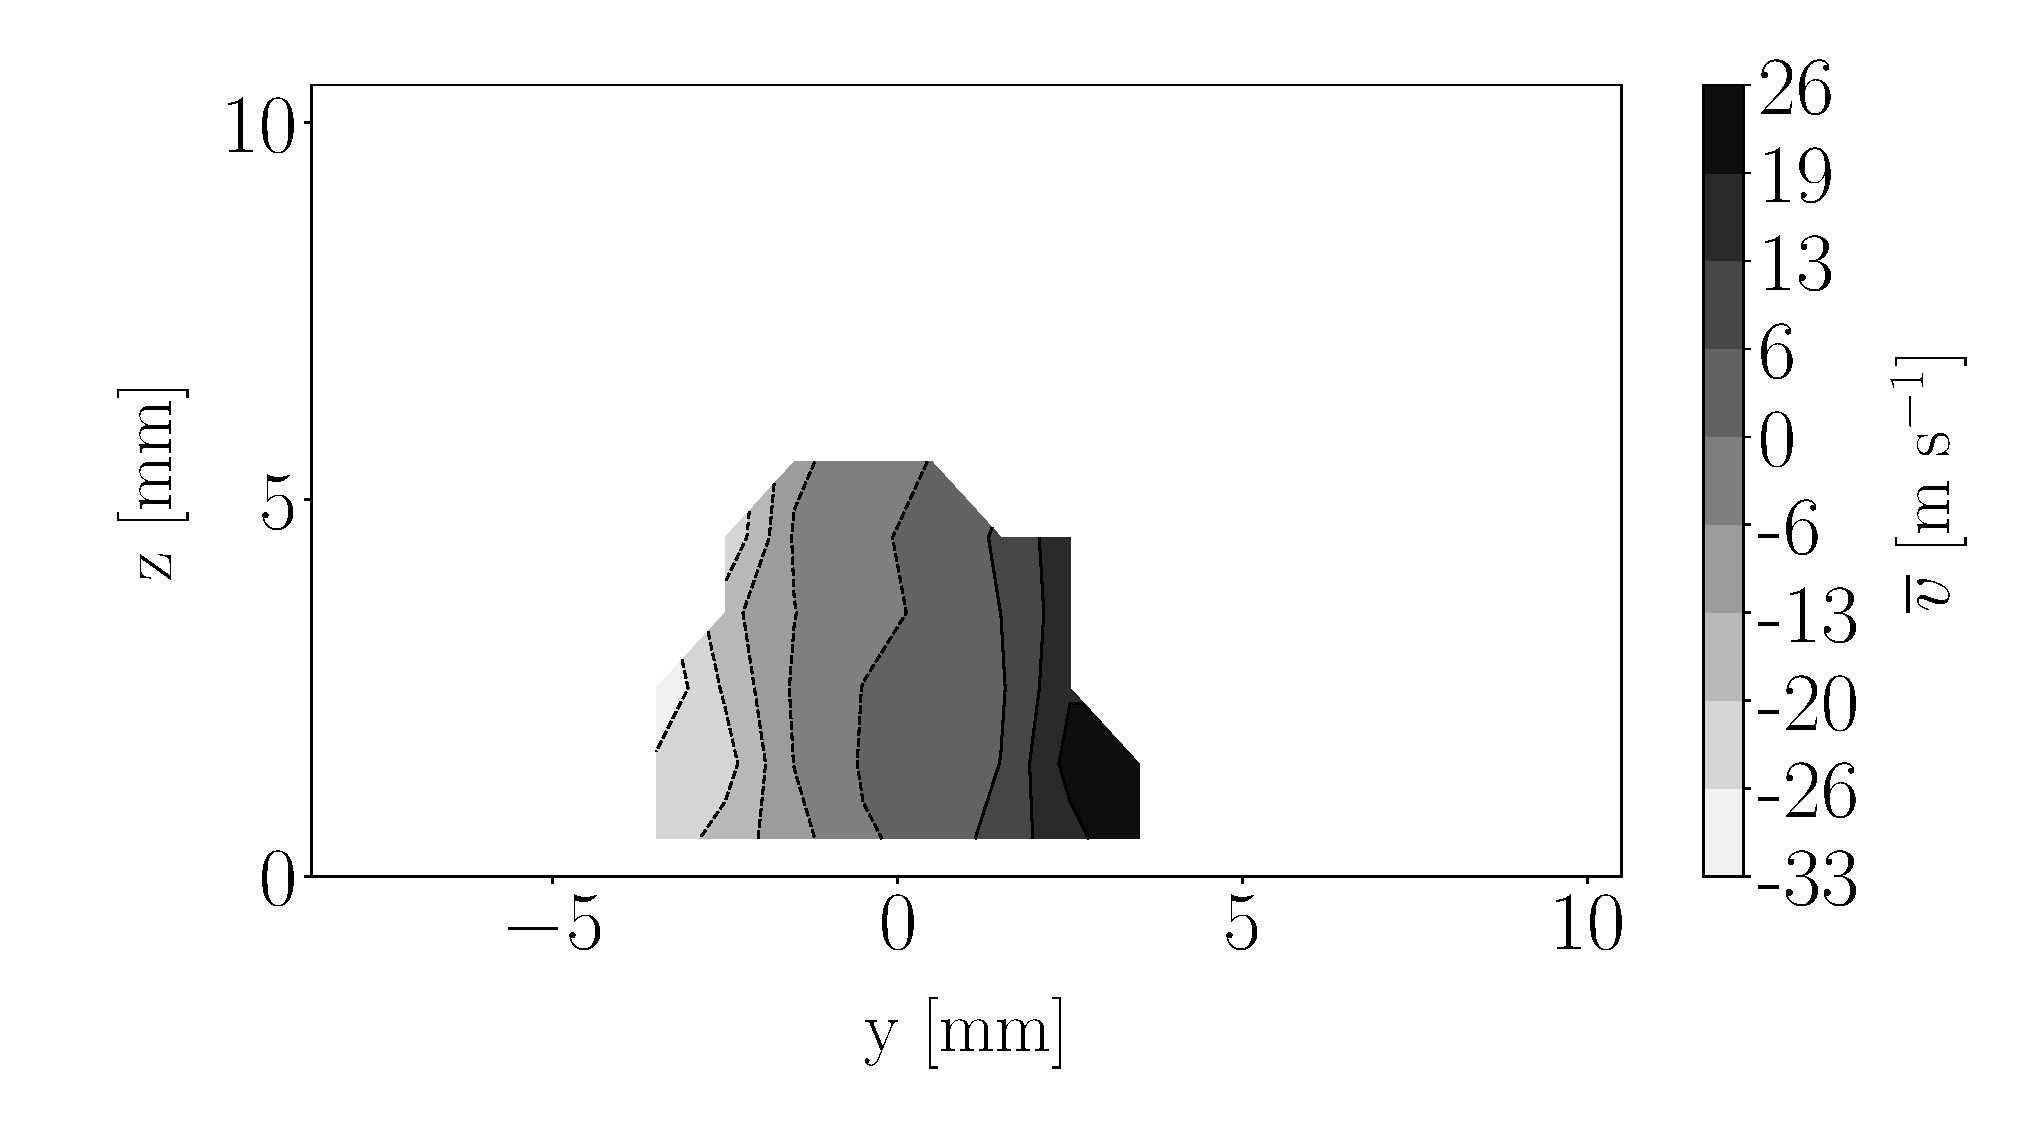
\includegraphics[scale=\scaleSLIJICF]{./part2_developments/figures_ch5_resolved_JICF/injectors_SLI/uG75_dx20_x05_uy_mean_map}
   %\caption{Case UG100\_DX20: filming planes}
   %\label{}
\end{subfigure}
   \hspace{0.17in}
\begin{subfigure}[b]{0.3\textwidth}
	\centering
   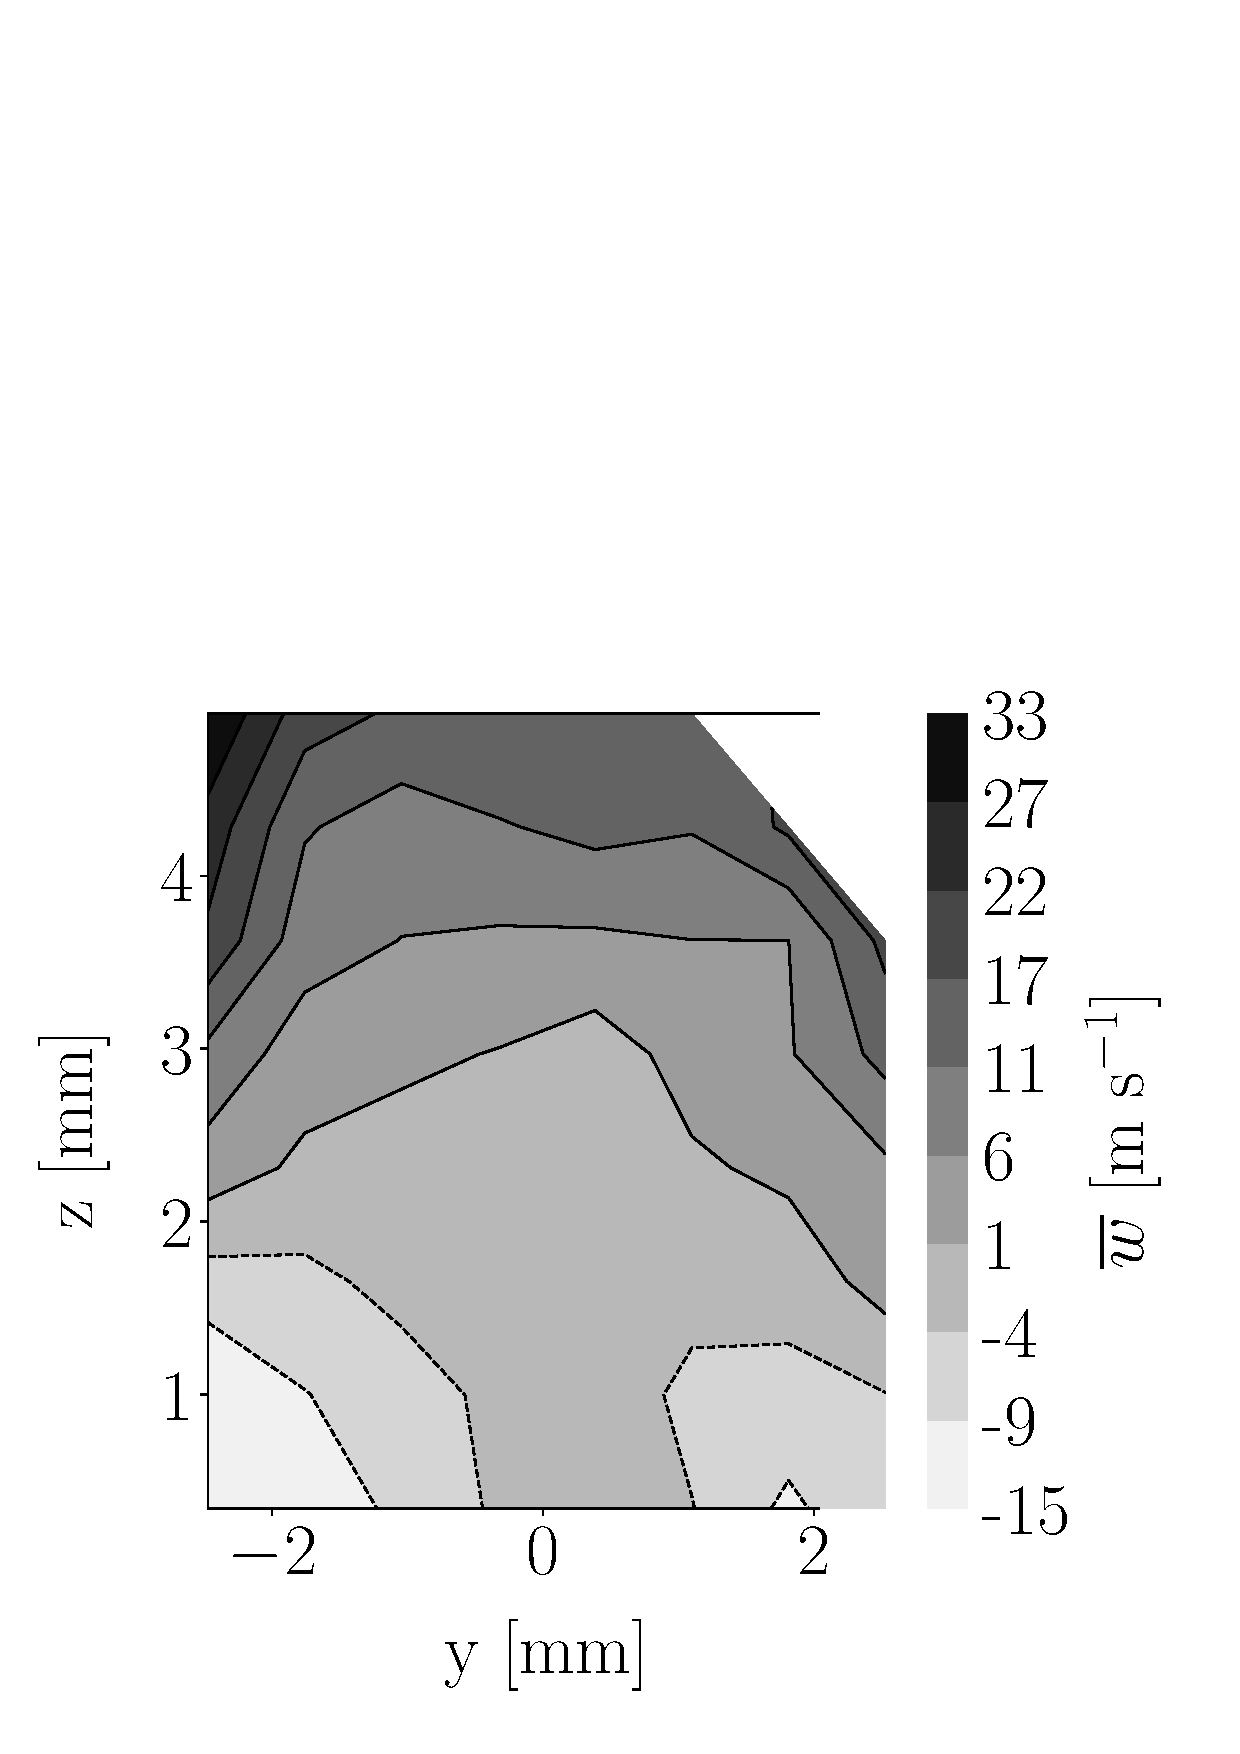
\includegraphics[scale=\scaleSLIJICF]{./part2_developments/figures_ch5_resolved_JICF/injectors_SLI/uG75_dx20_x05_uz_mean_map}
   %\caption{Case UG100\_DX10: crossflow planes}
   %\label{} 
\end{subfigure}
\caption{Spray states at x = 5 mm for case UG75\_DX20}
\label{fig:injectors_sli_uG75_dx20_x05}
\end{figure}


%%%%%%%%%%%%%%%% UG75_DX20, x = 10 mm


\begin{figure}[h!]
\centering
\begin{subfigure}[b]{0.3\textwidth}
	\centering
   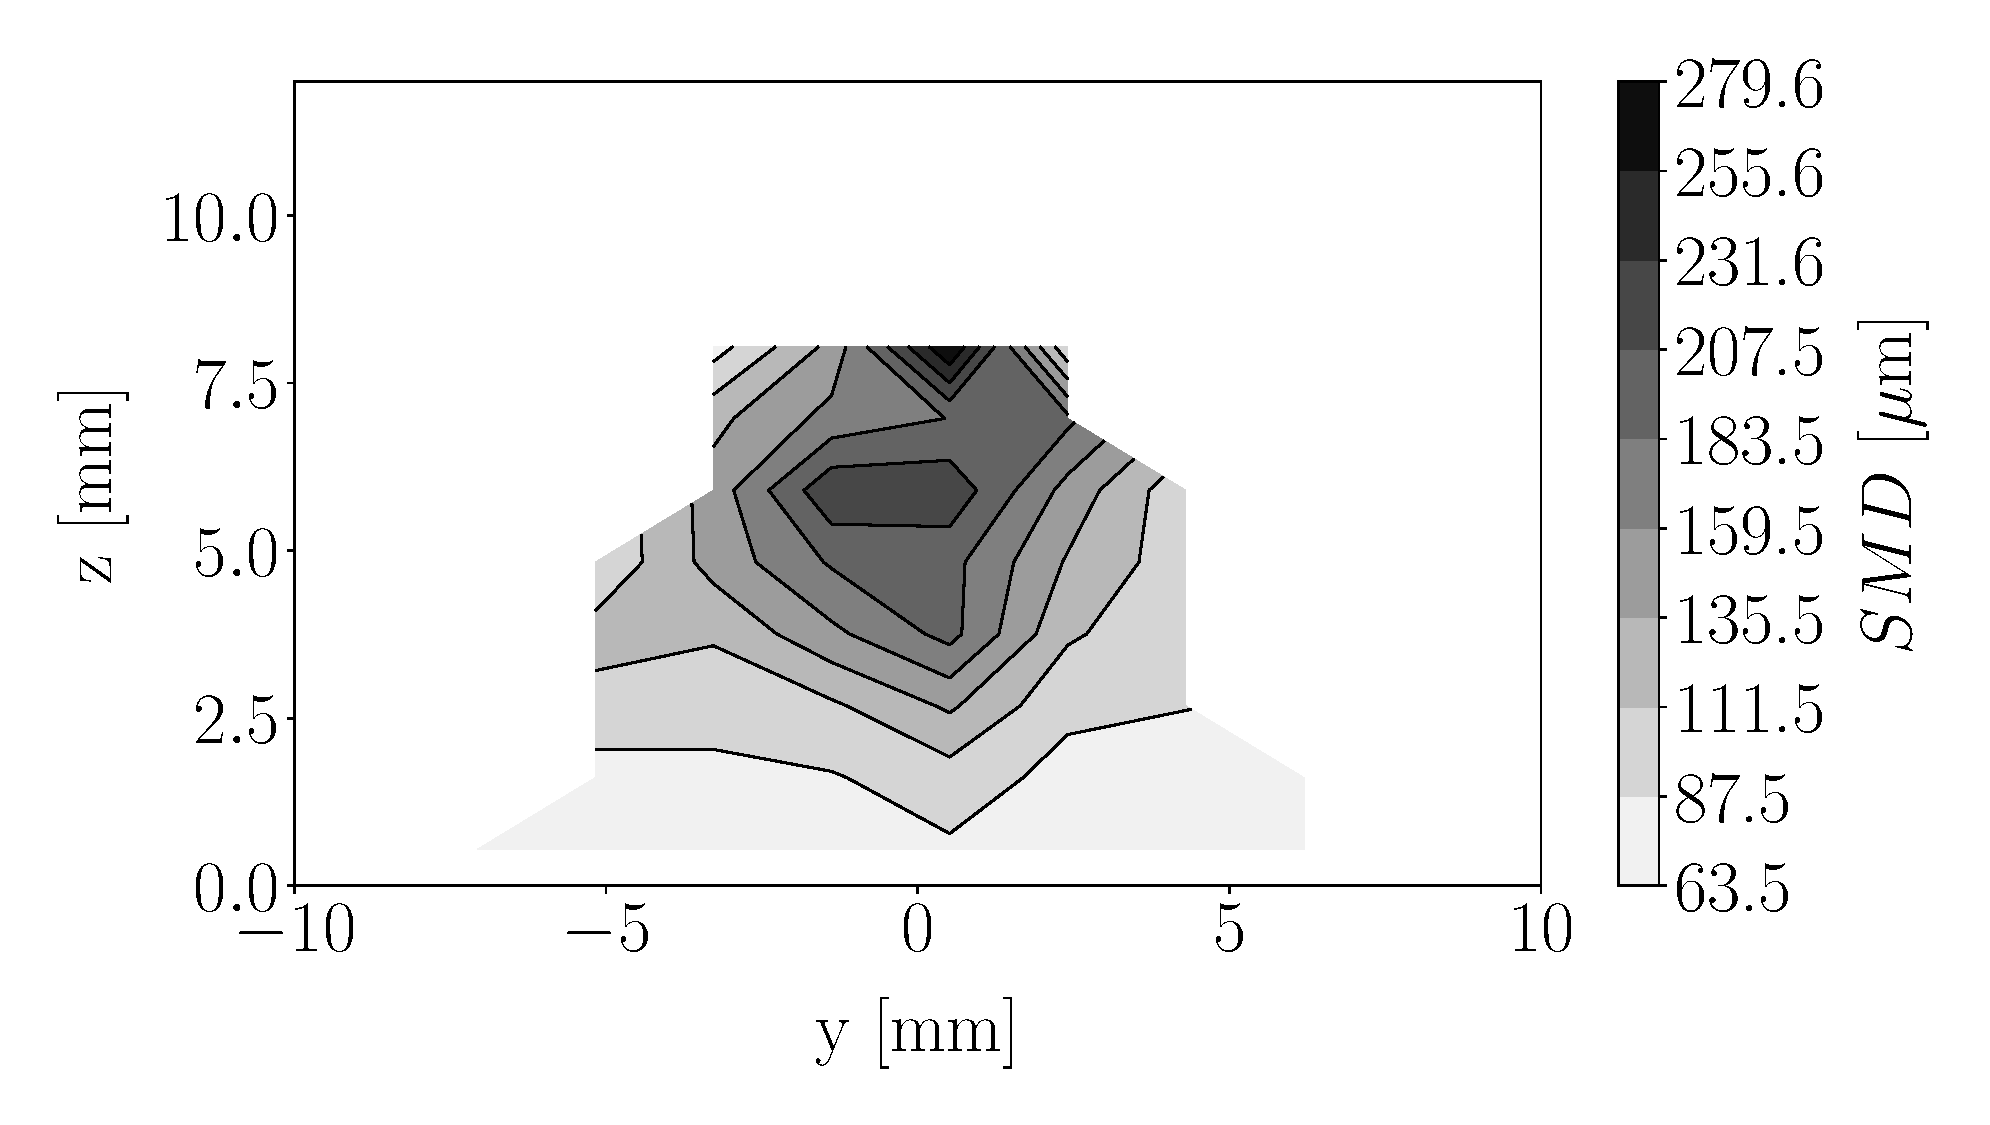
\includegraphics[scale=0.15]{./part2_developments/figures_ch5_resolved_JICF/injectors_SLI/uG75_dx20_x10_SMD_map}
   %\caption{Case UG100\_DX20: crossflow planes}
   %\label{} 
\end{subfigure}
   \hspace{0.17in}
\begin{subfigure}[b]{0.3\textwidth}
	\centering
   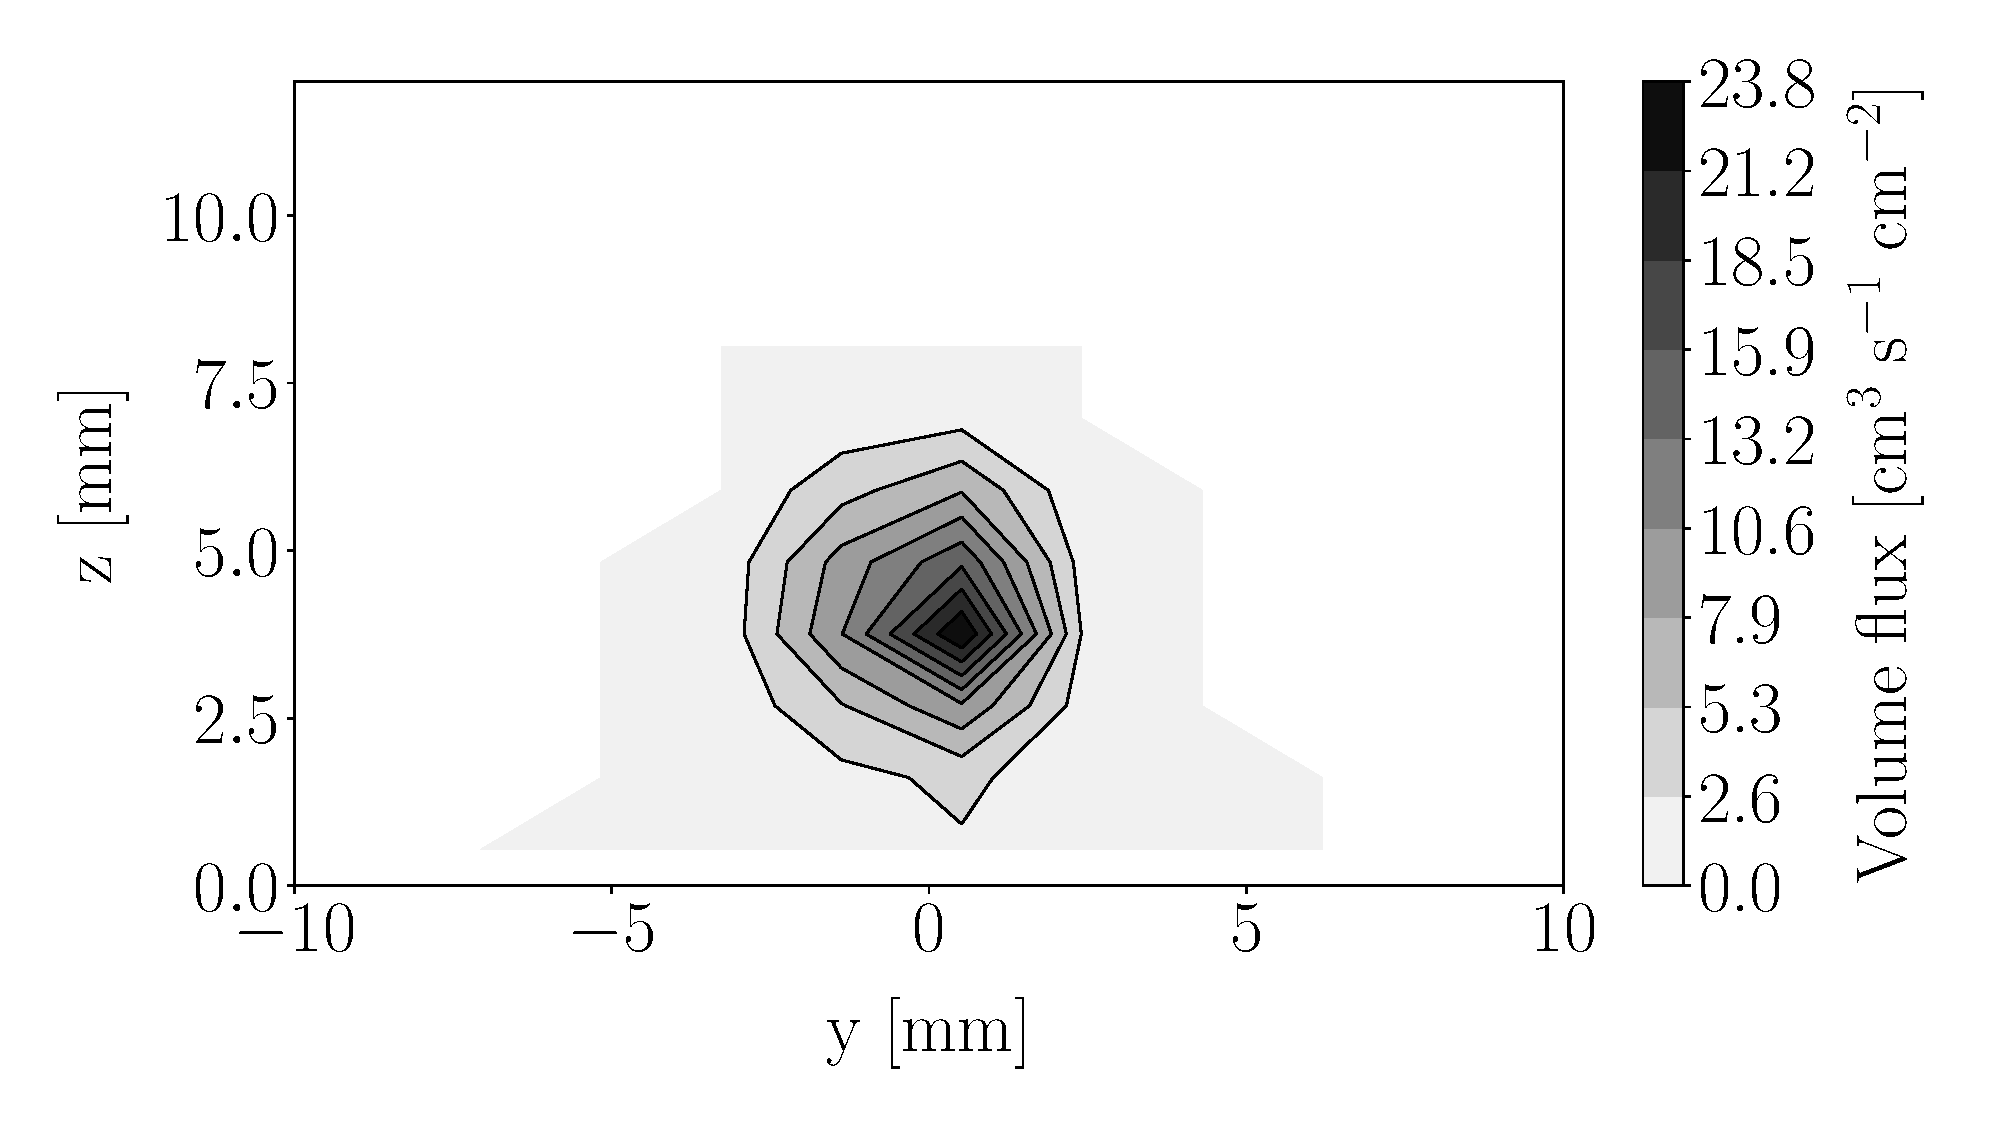
\includegraphics[scale=0.15]{./part2_developments/figures_ch5_resolved_JICF/injectors_SLI/uG75_dx20_x10_volume_flux_map}
   %\caption{Case UG100\_DX20: filming planes}
   %\label{}
\end{subfigure}
   \hspace{0.17in}
\begin{subfigure}[b]{0.3\textwidth}
	\centering
   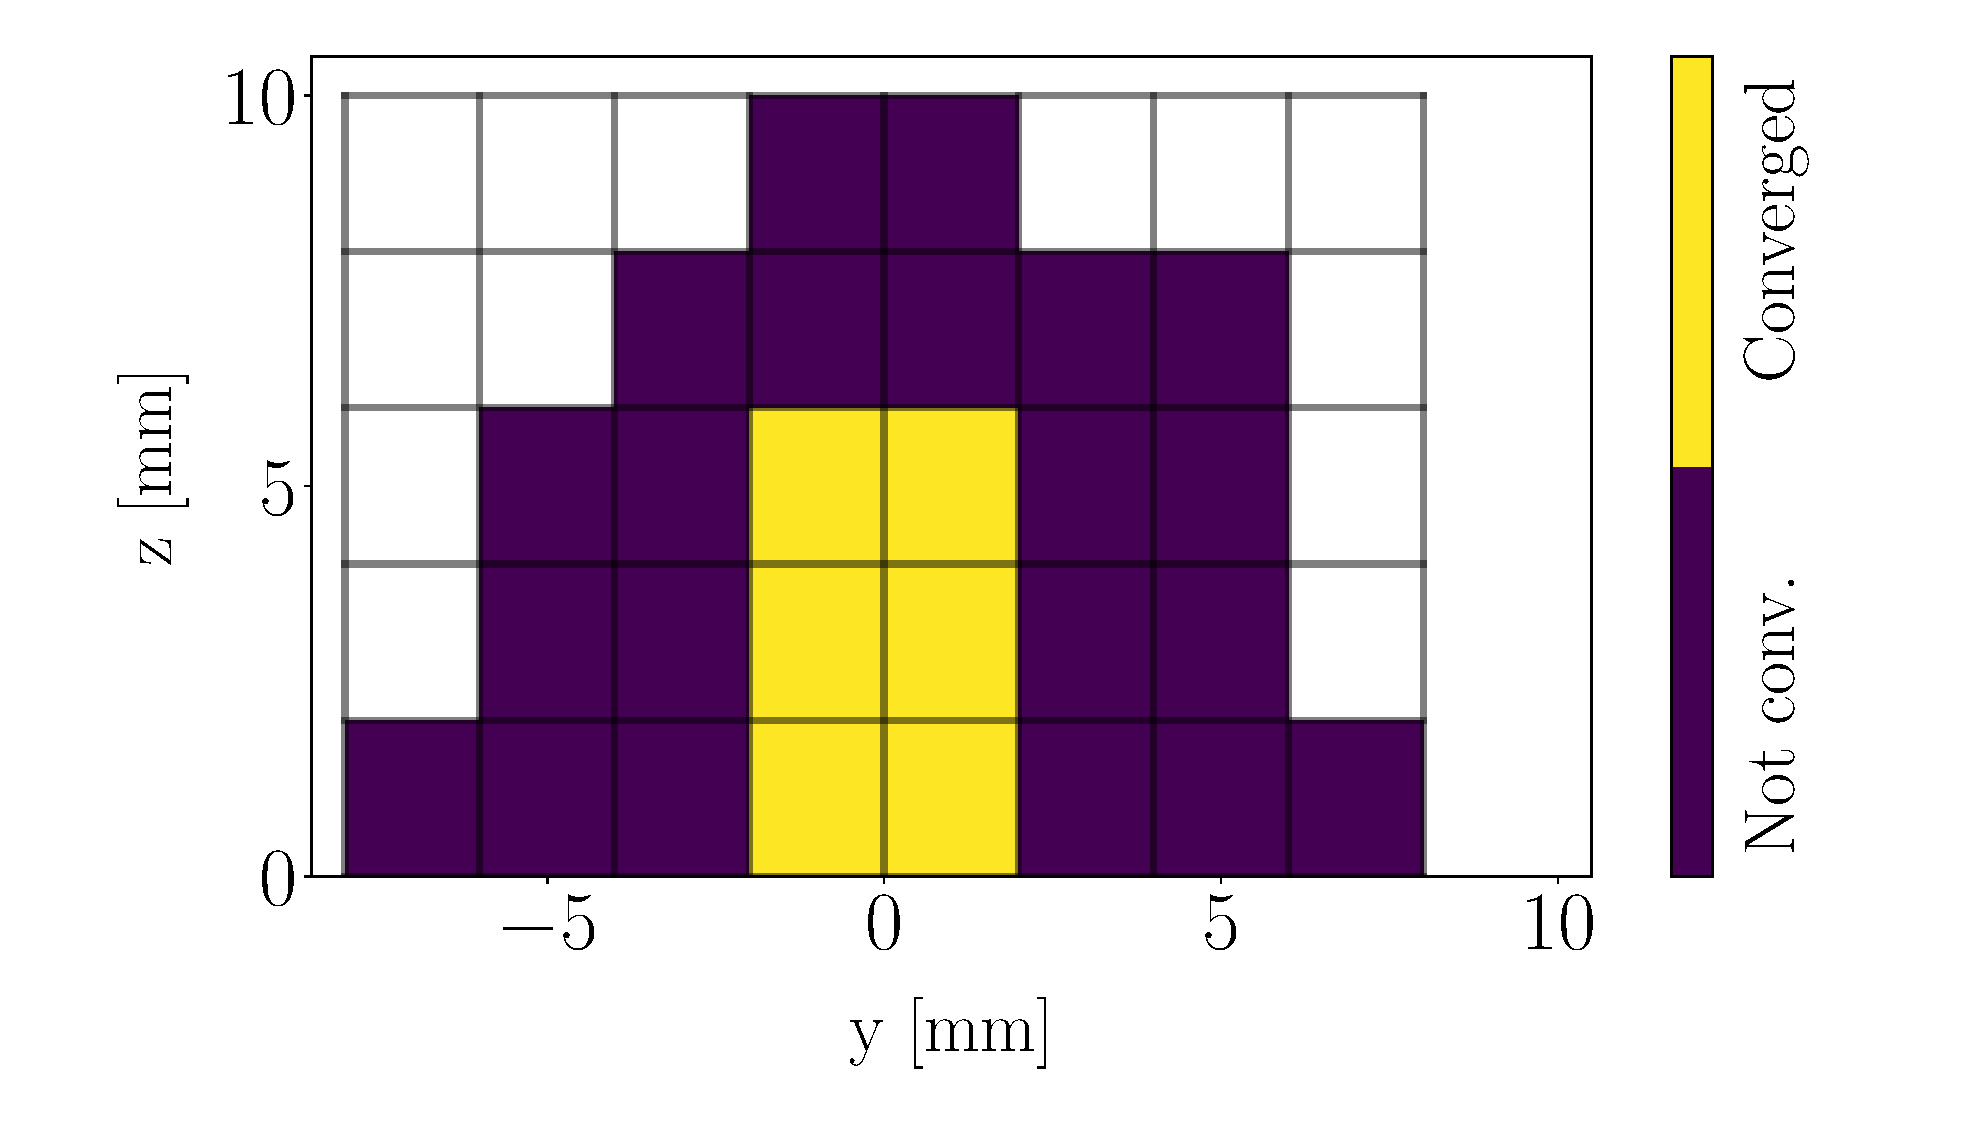
\includegraphics[scale=0.15]{./part2_developments/figures_ch5_resolved_JICF/injectors_SLI/uG75_dx20_x10_convergence_map}
   %\caption{Case UG100\_DX10: crossflow planes}
   %\label{} 
\end{subfigure}

\vskip\baselineskip

\begin{subfigure}[b]{0.3\textwidth}
	\centering
   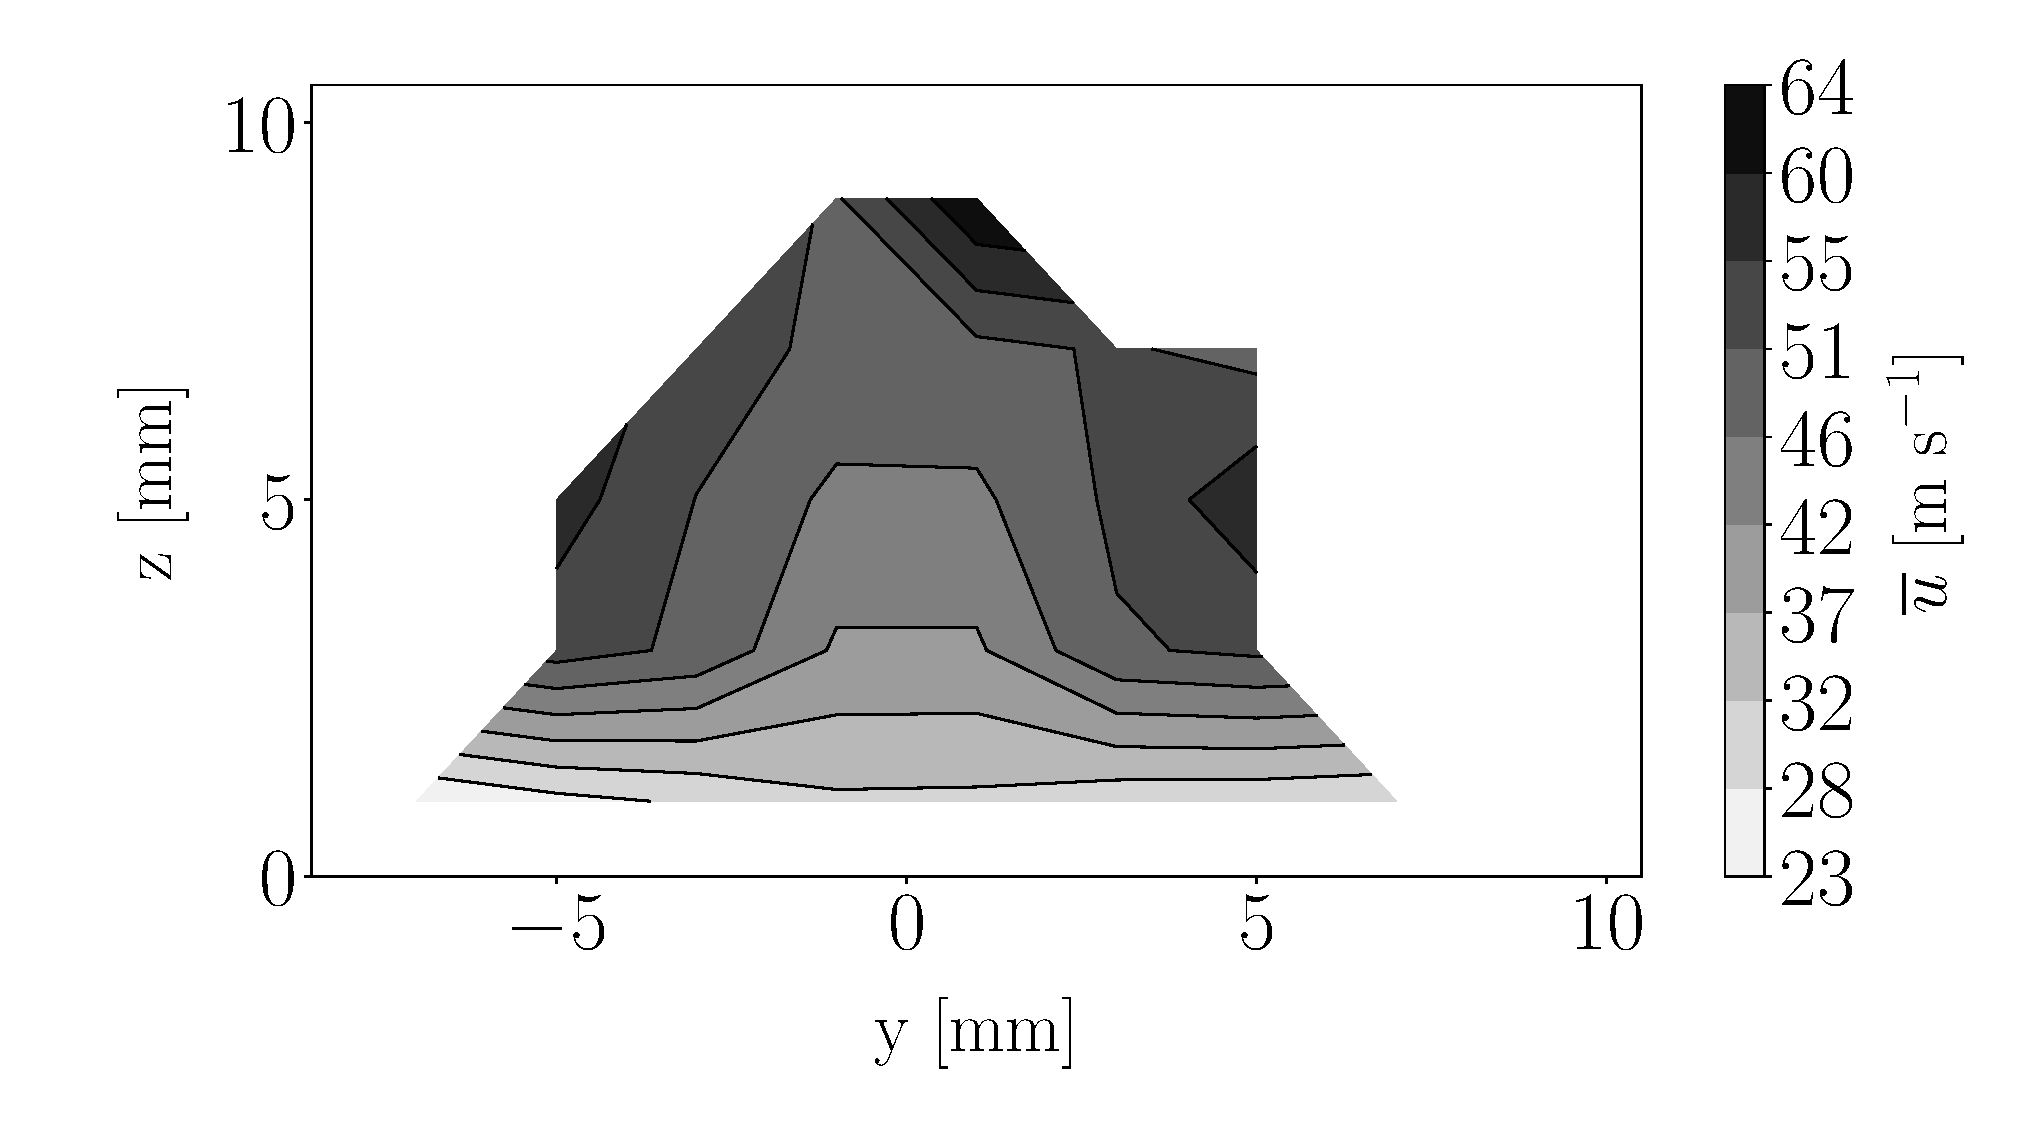
\includegraphics[scale=0.15]{./part2_developments/figures_ch5_resolved_JICF/injectors_SLI/uG75_dx20_x10_ux_mean_map}
   %\caption{Case UG100\_DX20: crossflow planes}
   %\label{} 
\end{subfigure}
   \hspace{0.17in}
\begin{subfigure}[b]{0.3\textwidth}
	\centering
   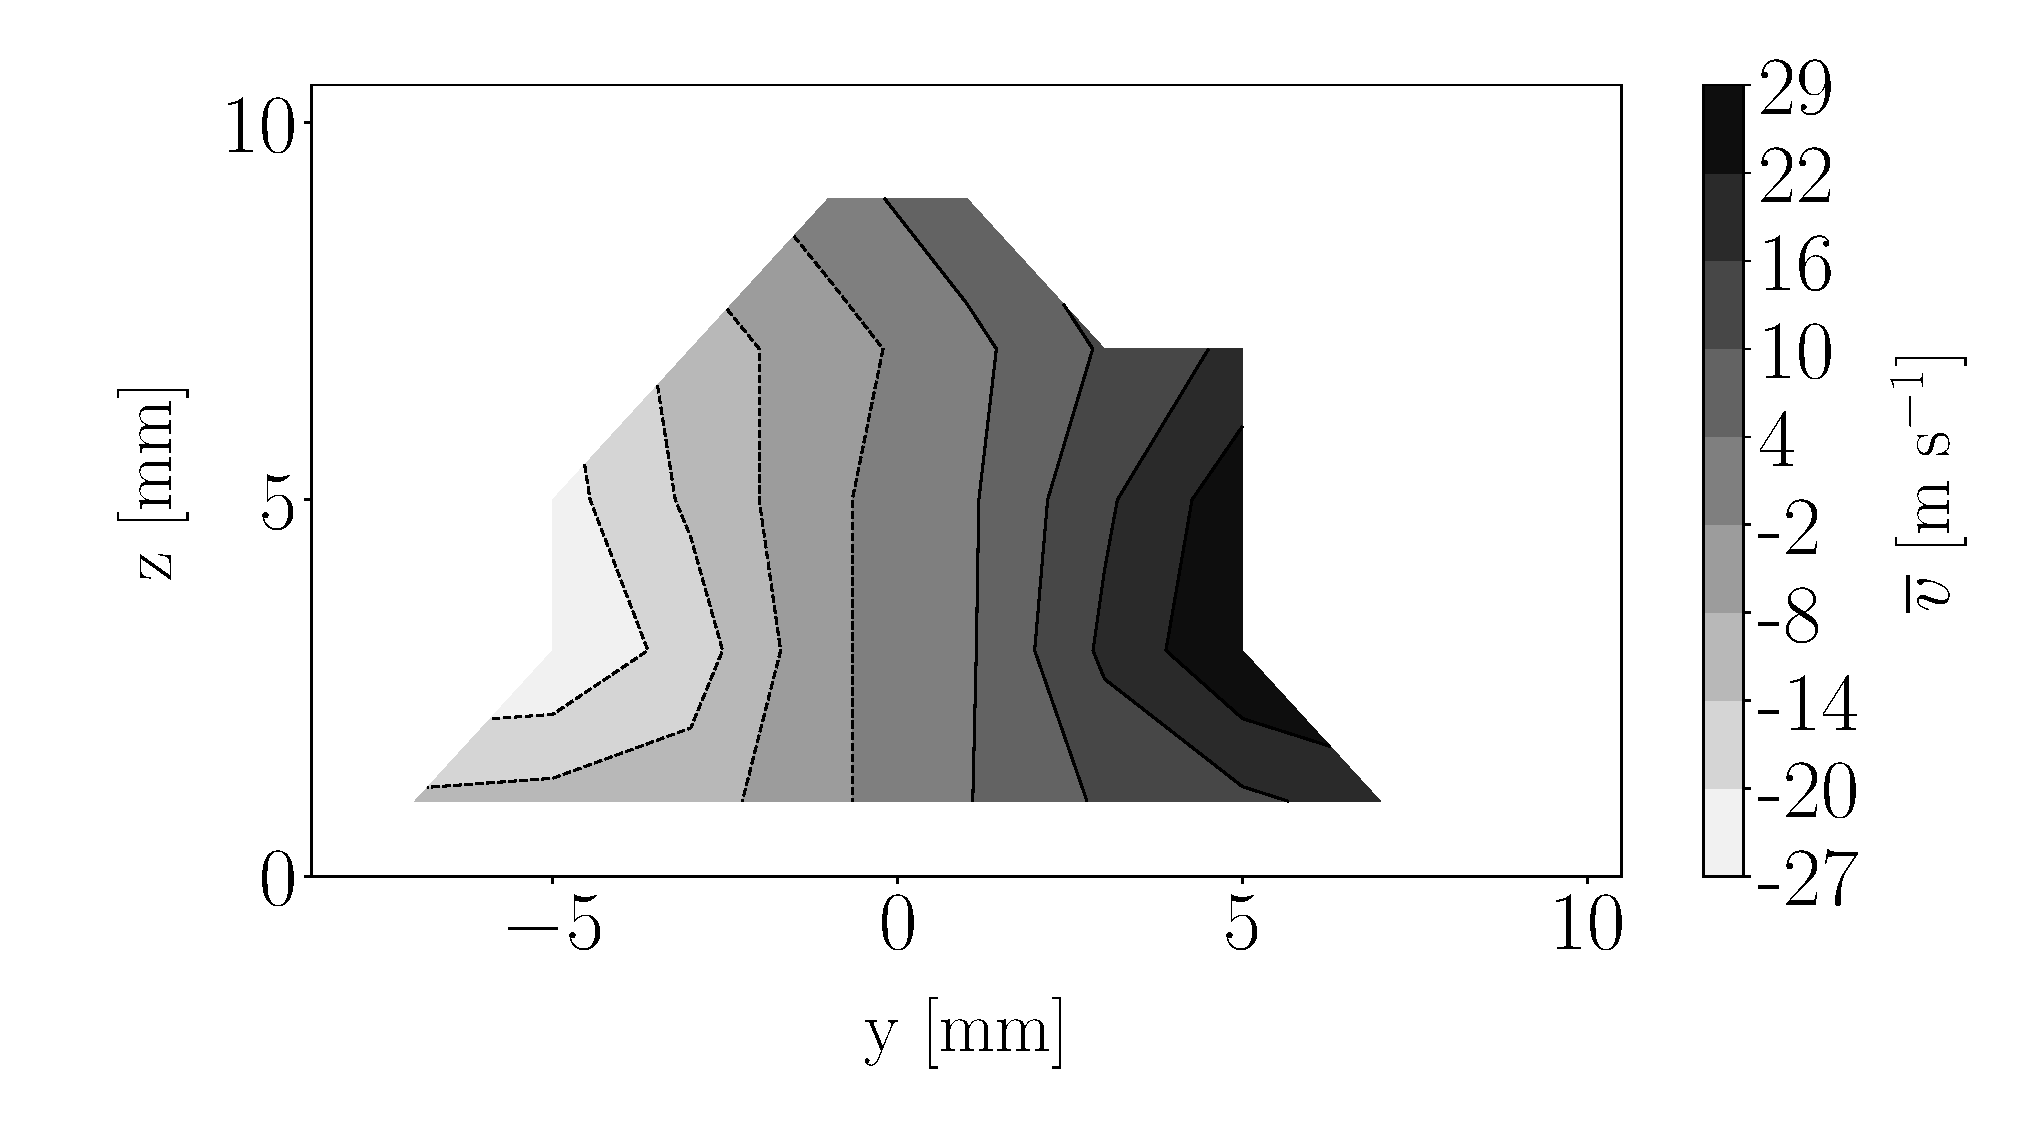
\includegraphics[scale=0.15]{./part2_developments/figures_ch5_resolved_JICF/injectors_SLI/uG75_dx20_x10_uy_mean_map}
   %\caption{Case UG100\_DX20: filming planes}
   %\label{}
\end{subfigure}
   \hspace{0.17in}
\begin{subfigure}[b]{0.3\textwidth}
	\centering
   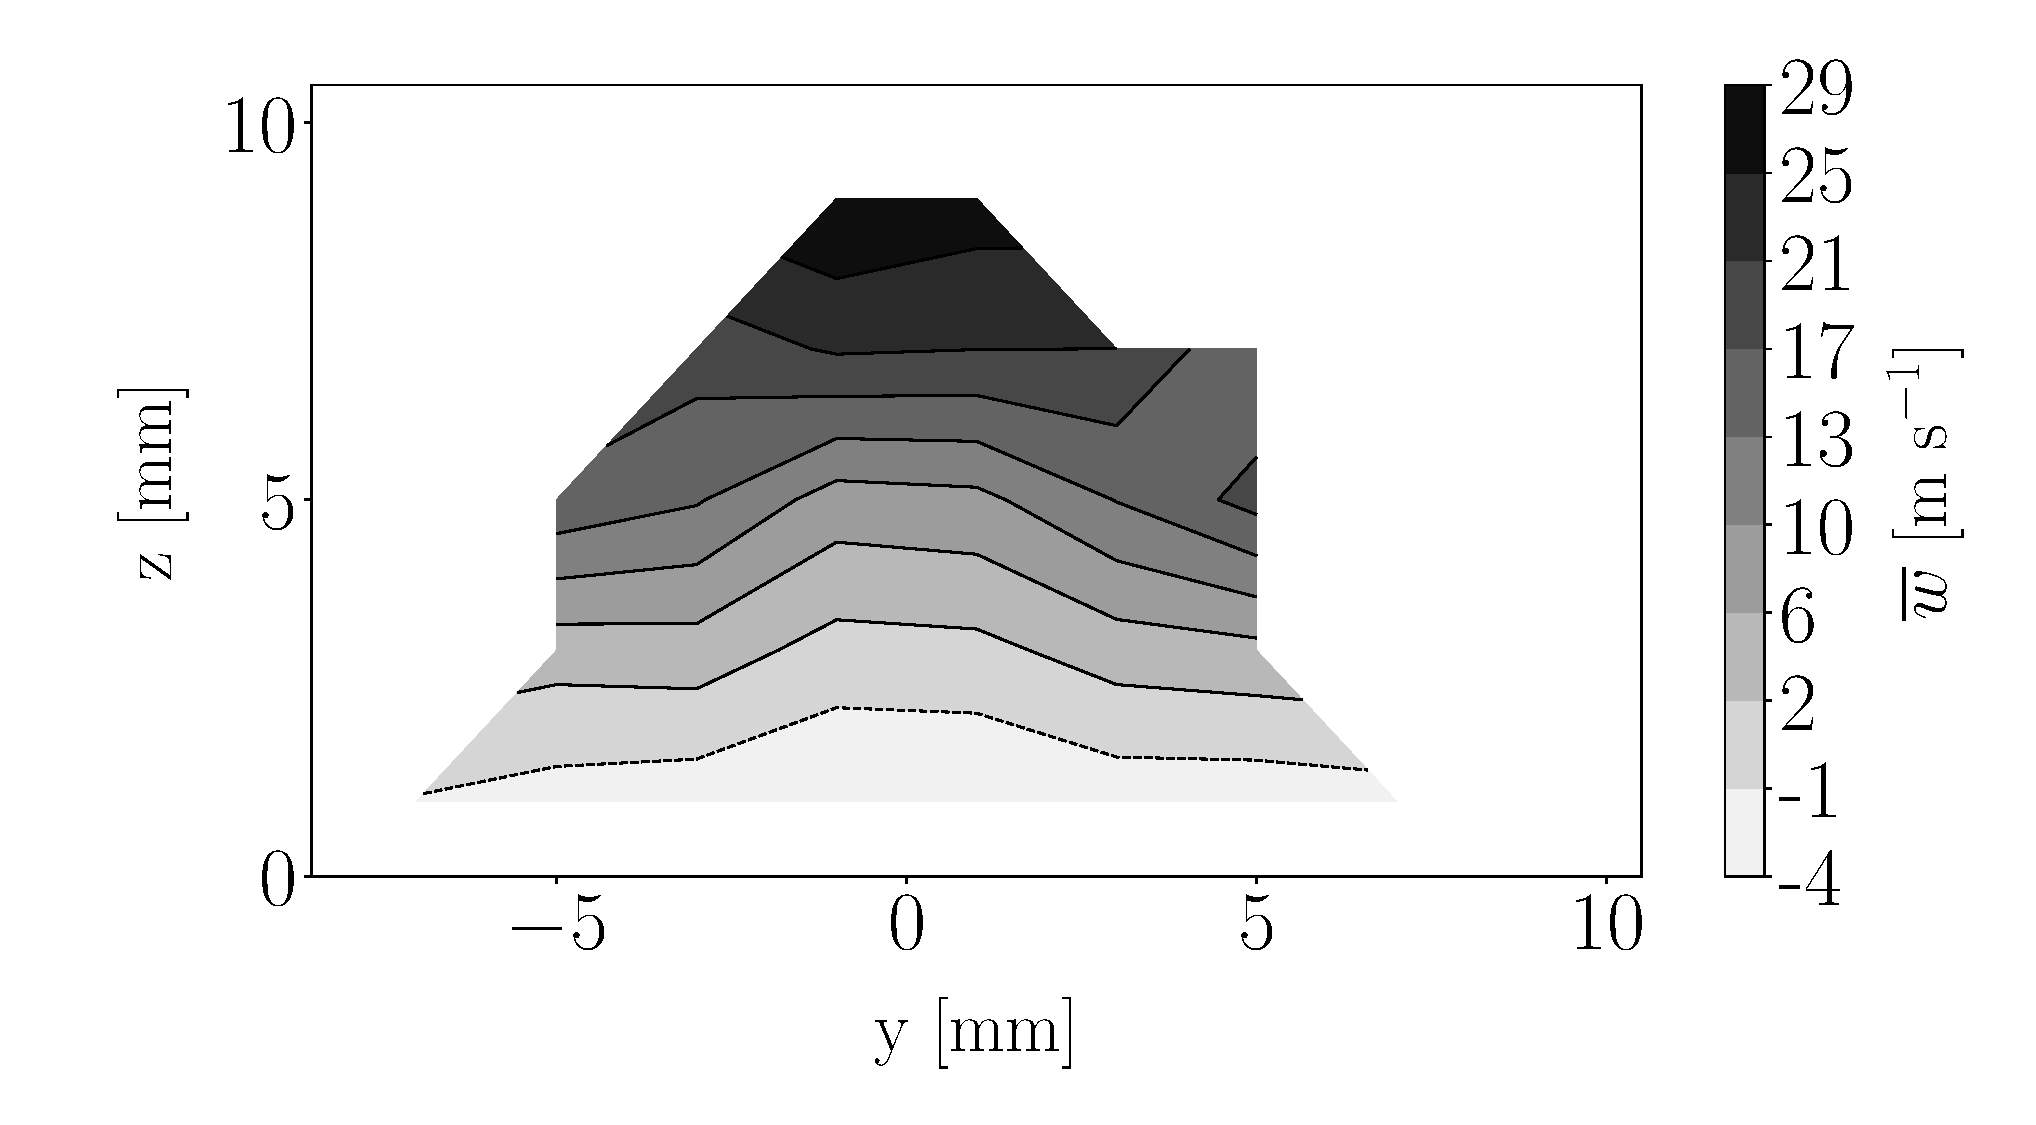
\includegraphics[scale=0.15]{./part2_developments/figures_ch5_resolved_JICF/injectors_SLI/uG75_dx20_x10_uz_mean_map}
   %\caption{Case UG100\_DX10: crossflow planes}
   %\label{} 
\end{subfigure}
\caption{Spray states at x = 10 mm for case UG75\_DX20}
\label{fig:injectors_sli_uG75_dx20_x10}
\end{figure}


%%%%%%%%%%%%%%%% UG75_DX10, x = 15 mm


\begin{figure}[h!]
\centering
\begin{subfigure}[b]{0.3\textwidth}
	\centering
   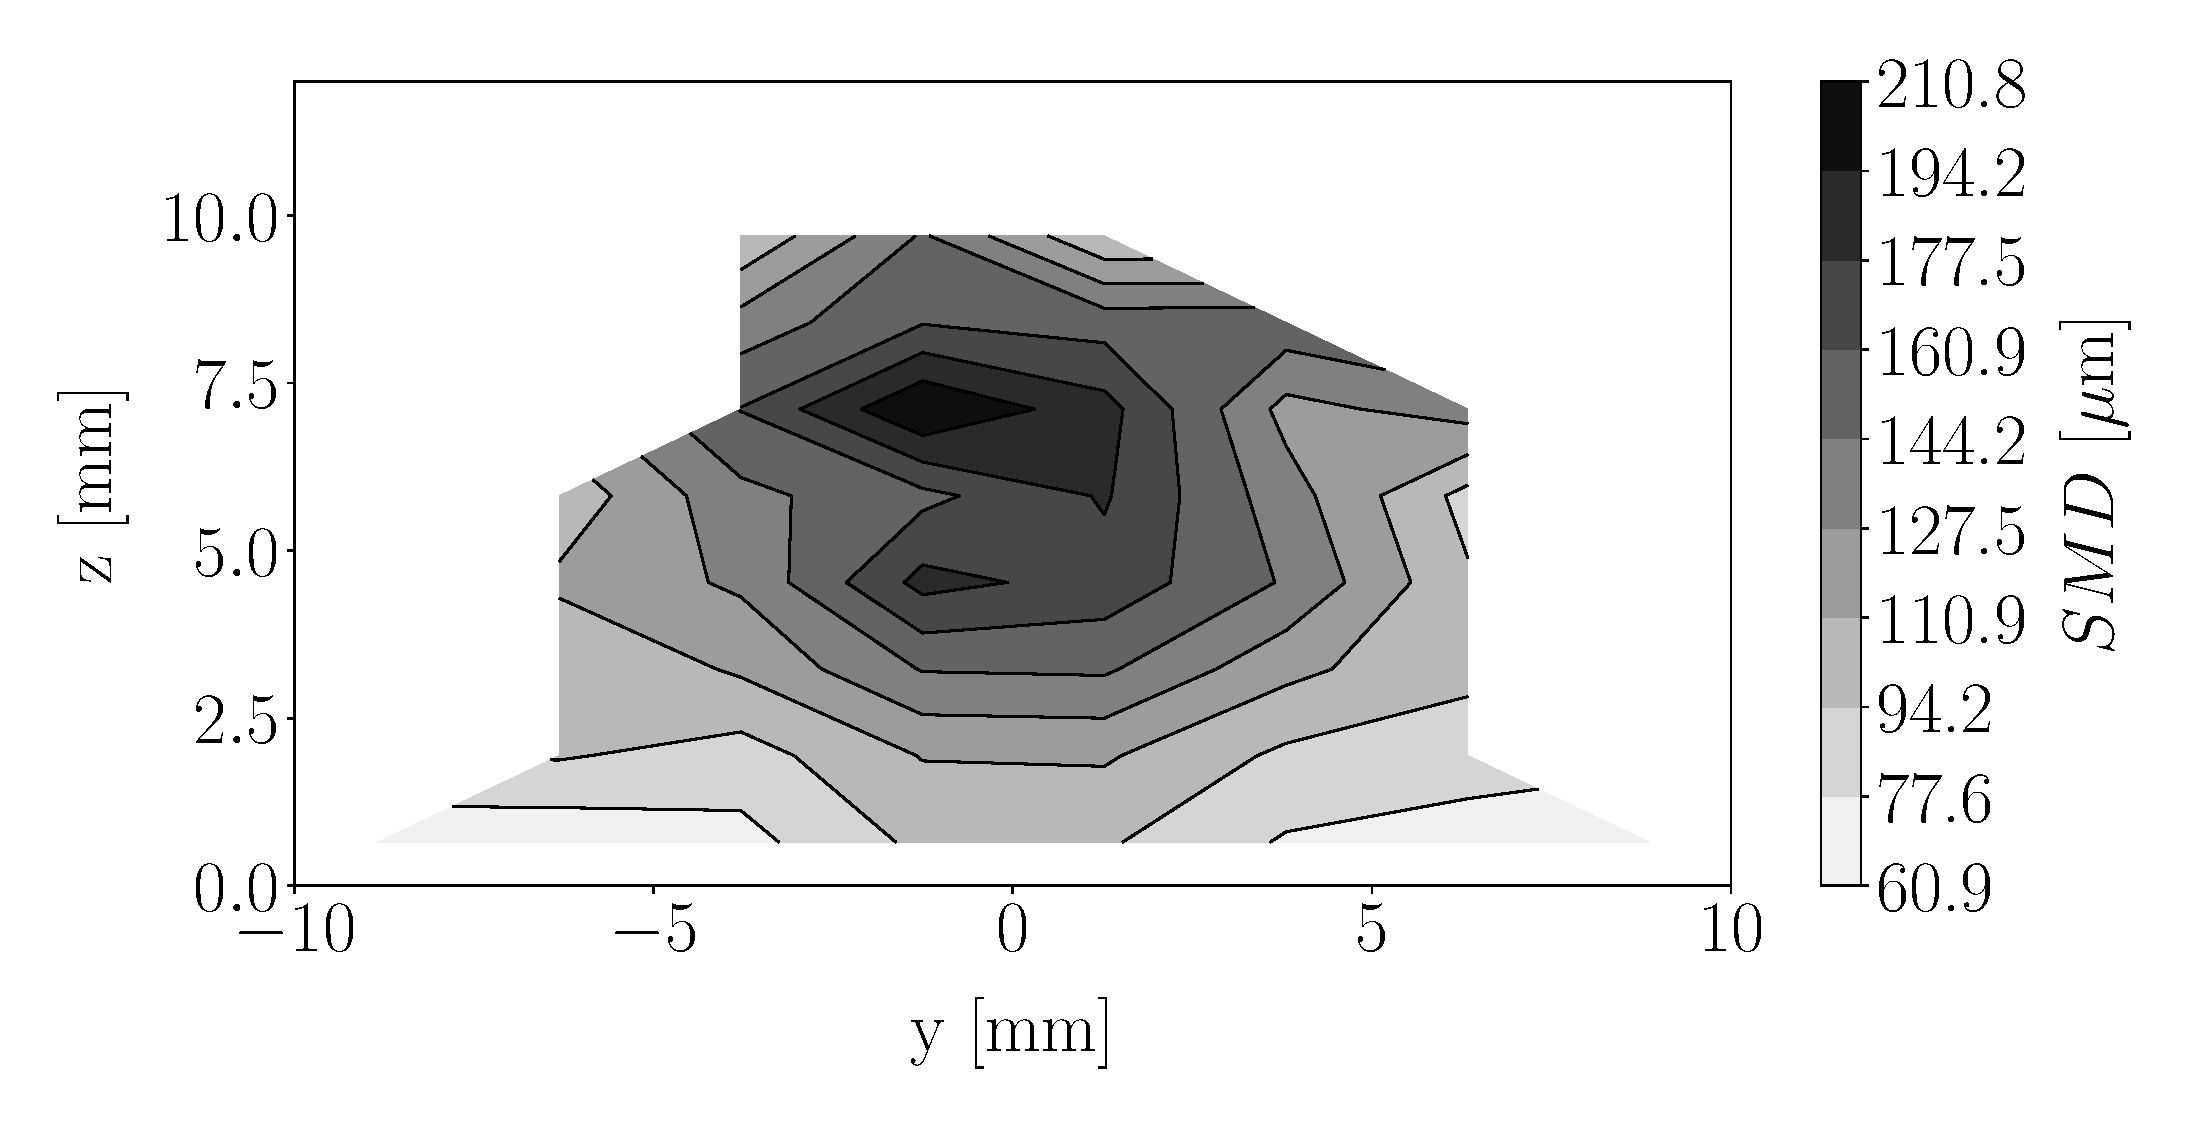
\includegraphics[scale=\scaleSLIJICF]{./part2_developments/figures_ch5_resolved_JICF/injectors_SLI/uG75_dx20_x15_SMD_map}
   %\caption{Case UG100\_DX20: crossflow planes}
   %\label{} 
\end{subfigure}
   \hspace{0.17in}
\begin{subfigure}[b]{0.3\textwidth}
	\centering
   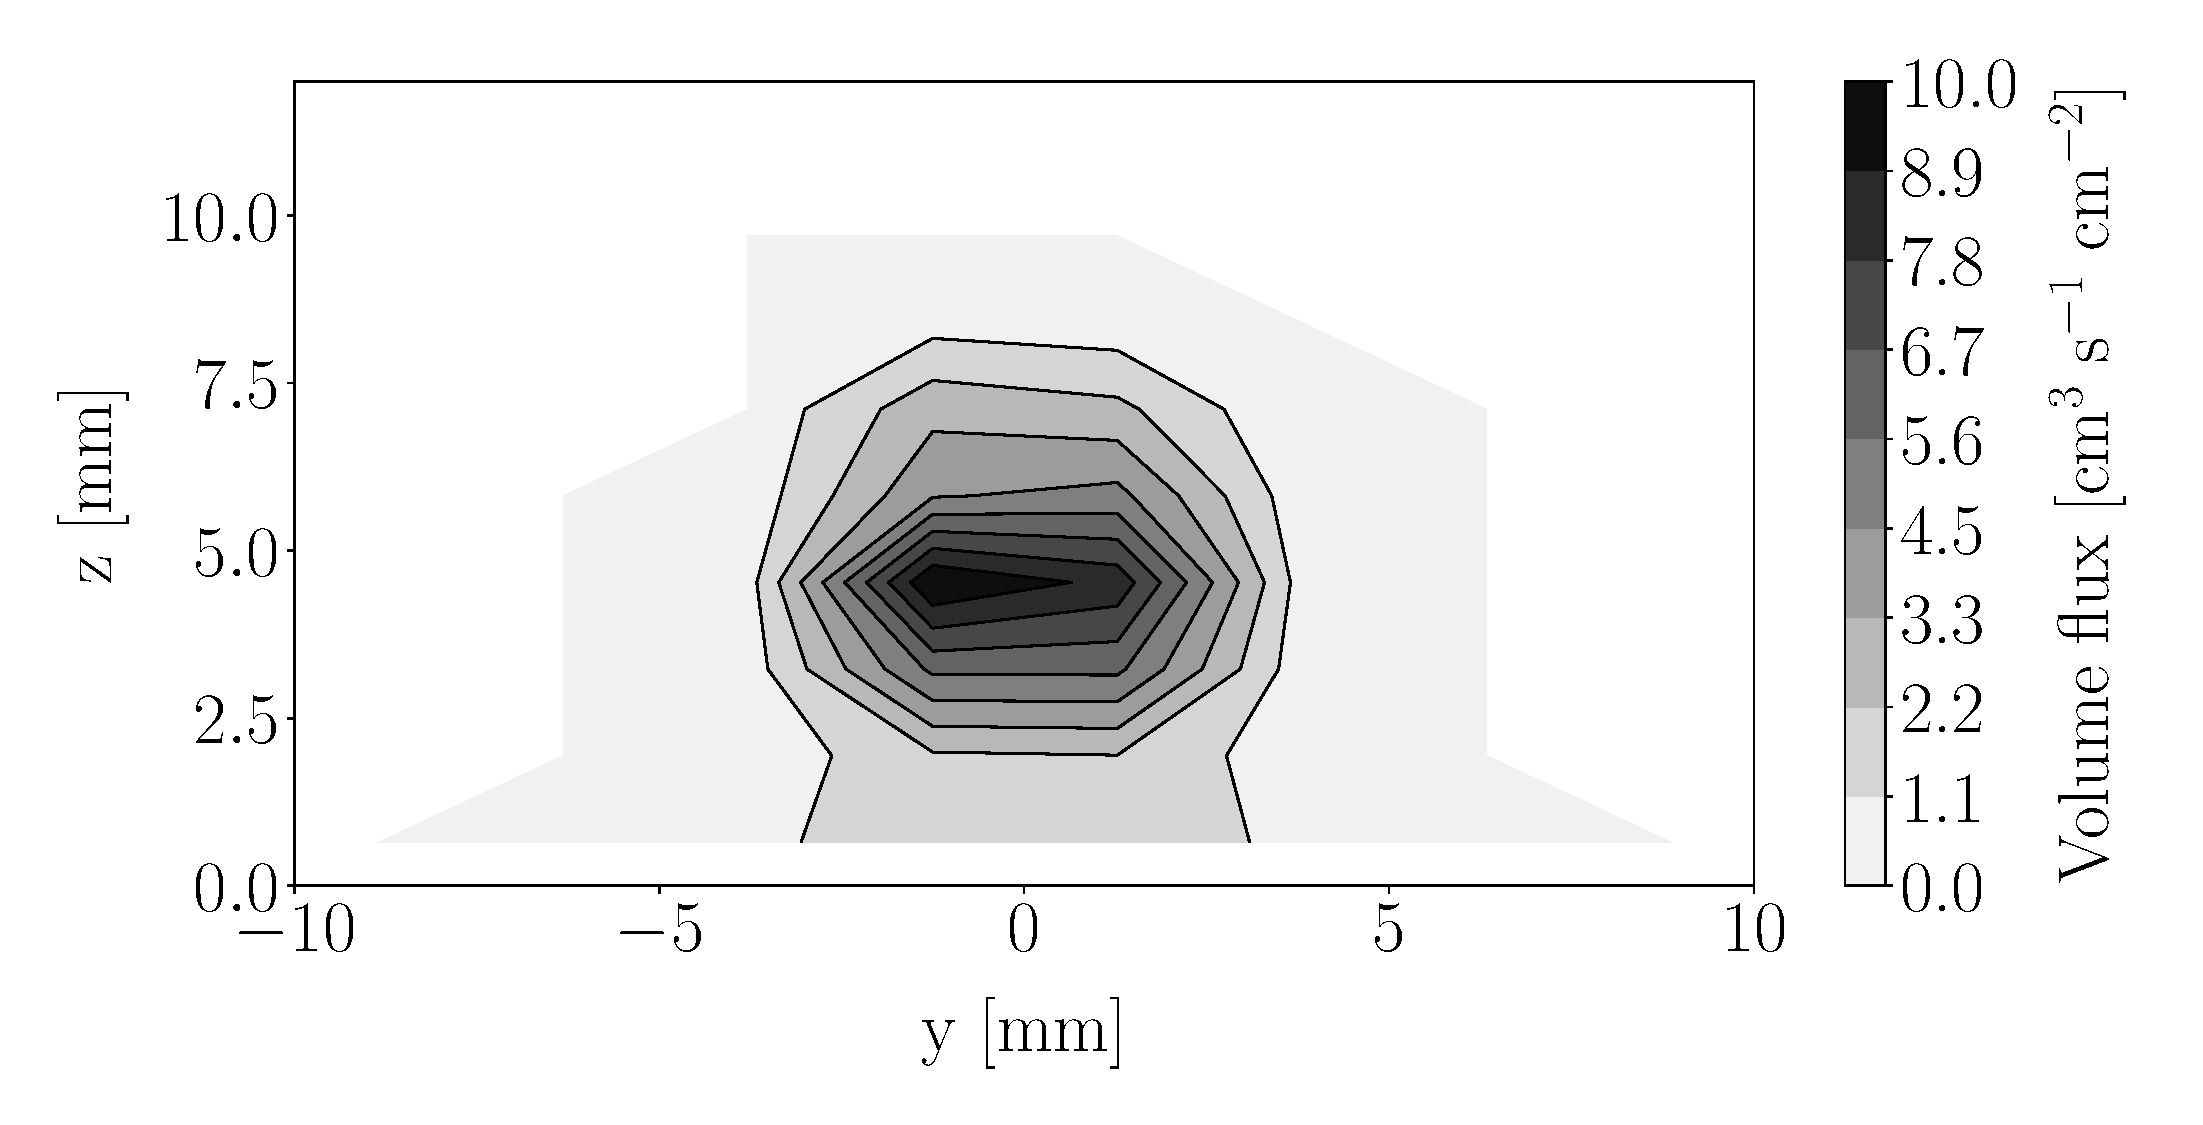
\includegraphics[scale=\scaleSLIJICF]{./part2_developments/figures_ch5_resolved_JICF/injectors_SLI/uG75_dx20_x15_volume_flux_map}
   %\caption{Case UG100\_DX20: filming planes}
   %\label{}
\end{subfigure}
   \hspace{0.17in}
\begin{subfigure}[b]{0.3\textwidth}
	\centering
   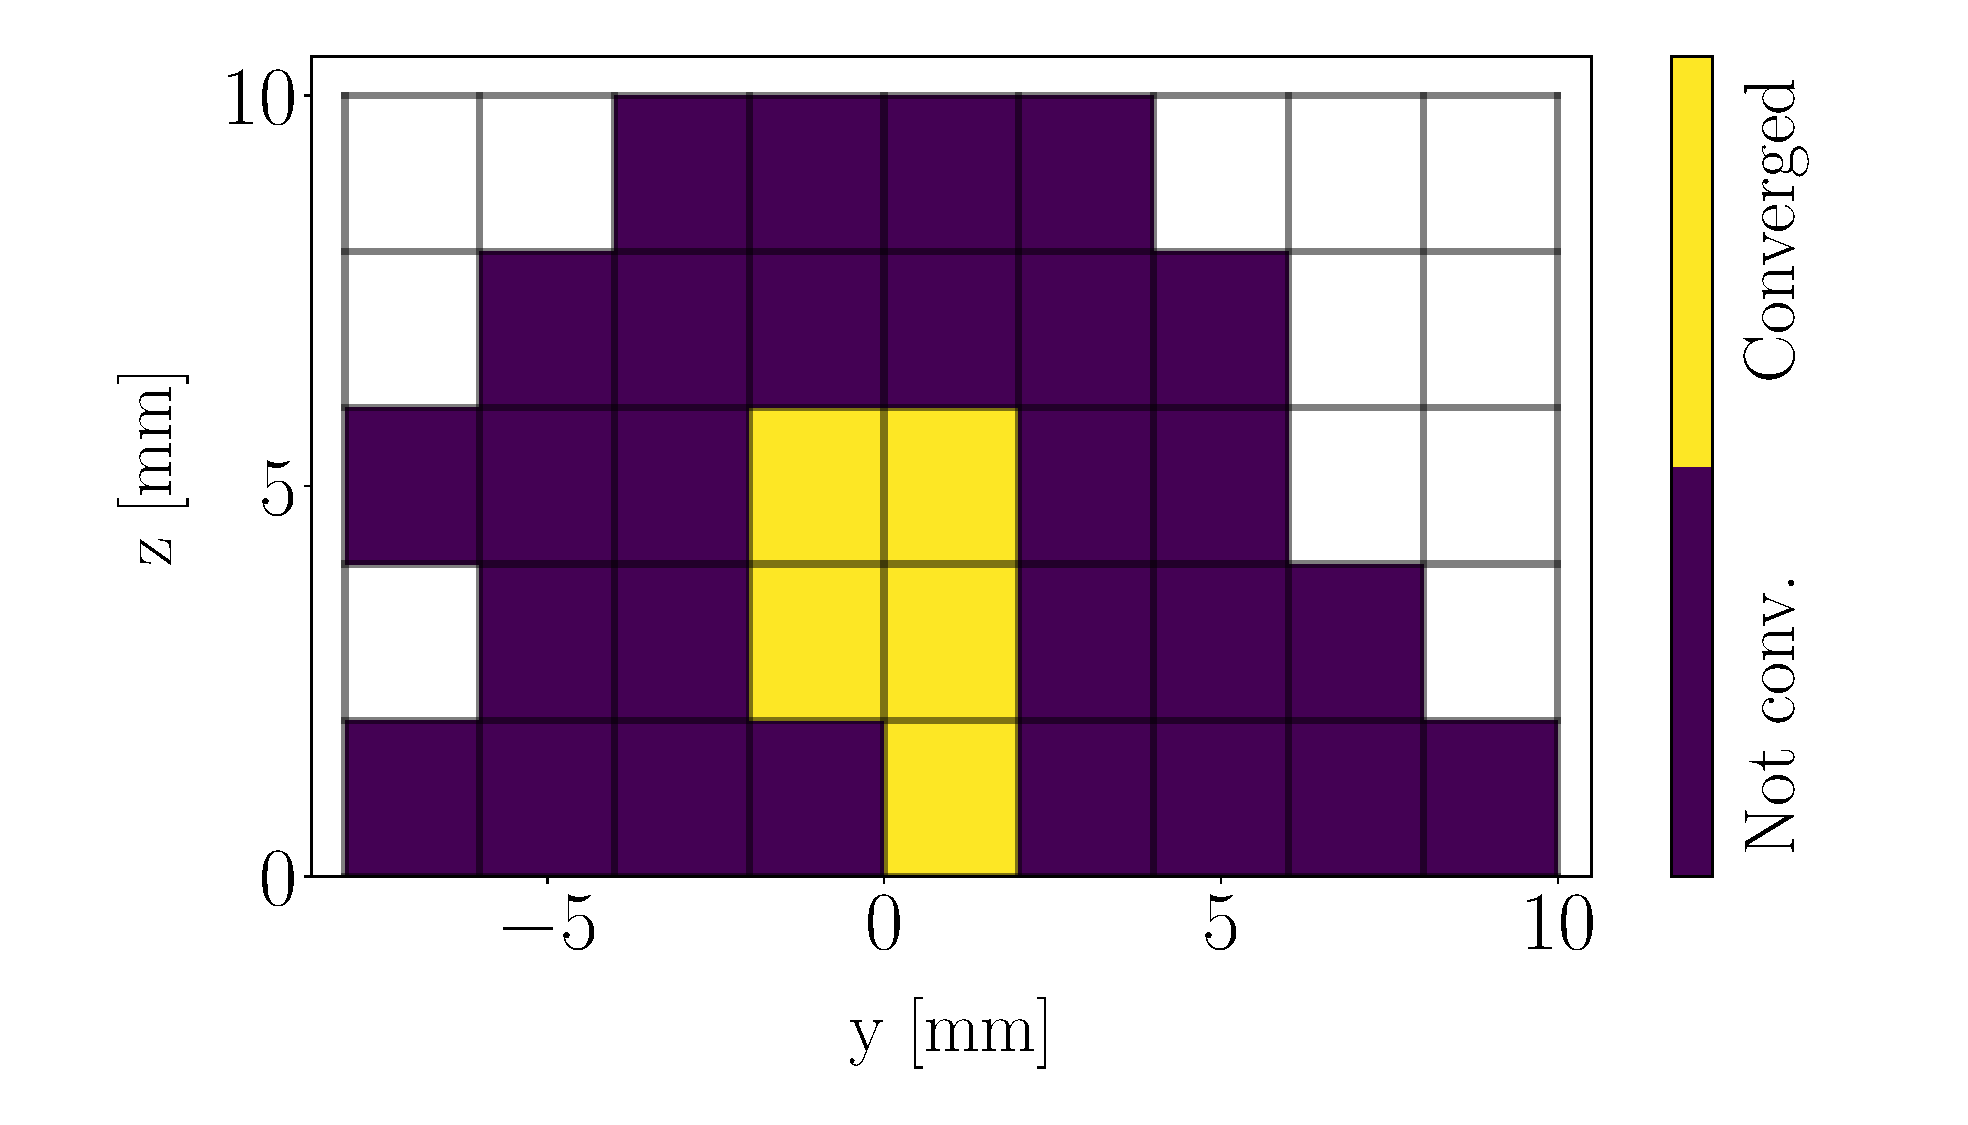
\includegraphics[scale=\scaleSLIJICF]{./part2_developments/figures_ch5_resolved_JICF/injectors_SLI/uG75_dx20_x15_convergence_map}
   %\caption{Case UG100\_DX10: crossflow planes}
   %\label{} 
\end{subfigure}

\vskip\baselineskip

\begin{subfigure}[b]{0.3\textwidth}
	\centering
   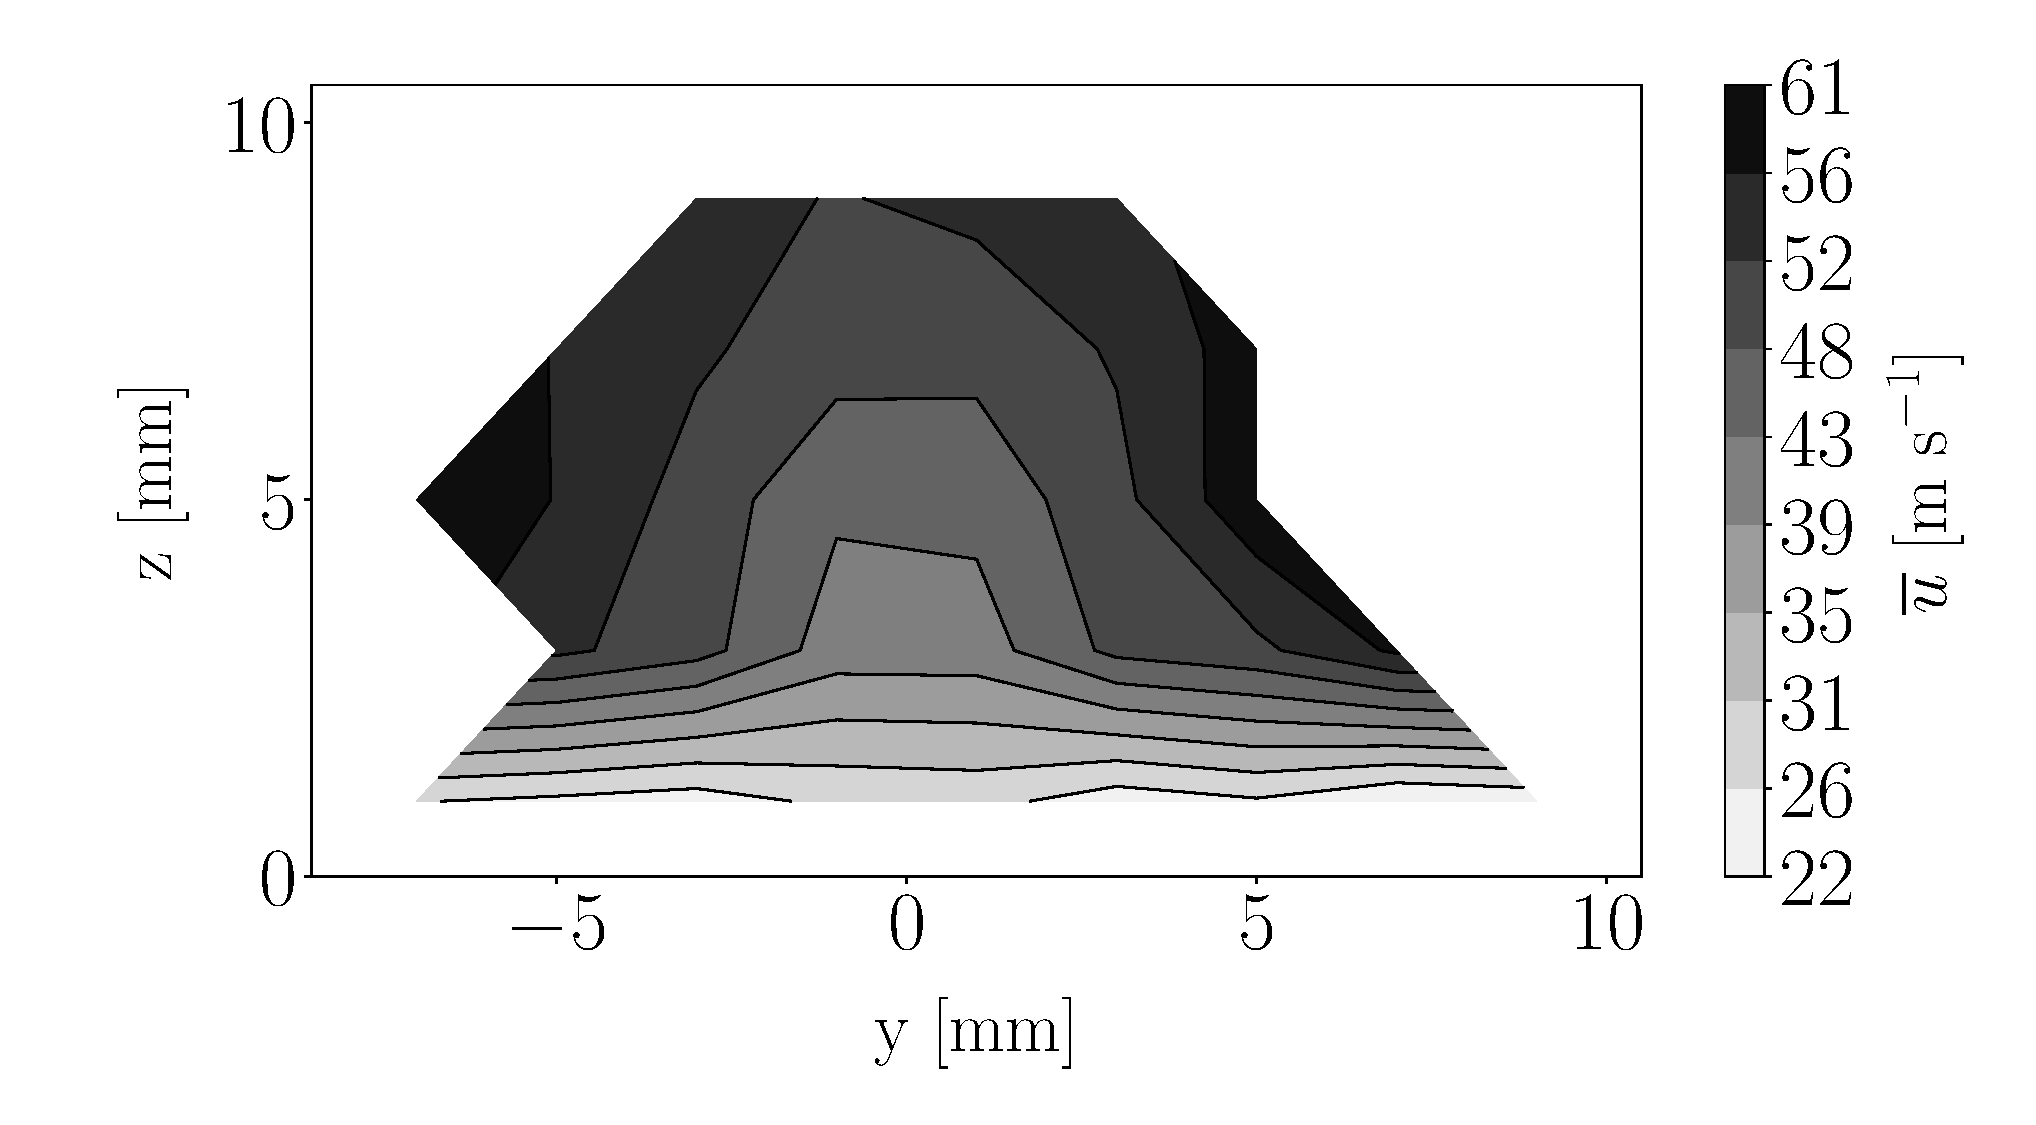
\includegraphics[scale=\scaleSLIJICF]{./part2_developments/figures_ch5_resolved_JICF/injectors_SLI/uG75_dx20_x15_ux_mean_map}
   %\caption{Case UG100\_DX20: crossflow planes}
   %\label{} 
\end{subfigure}
   \hspace{0.17in}
\begin{subfigure}[b]{0.3\textwidth}
	\centering
   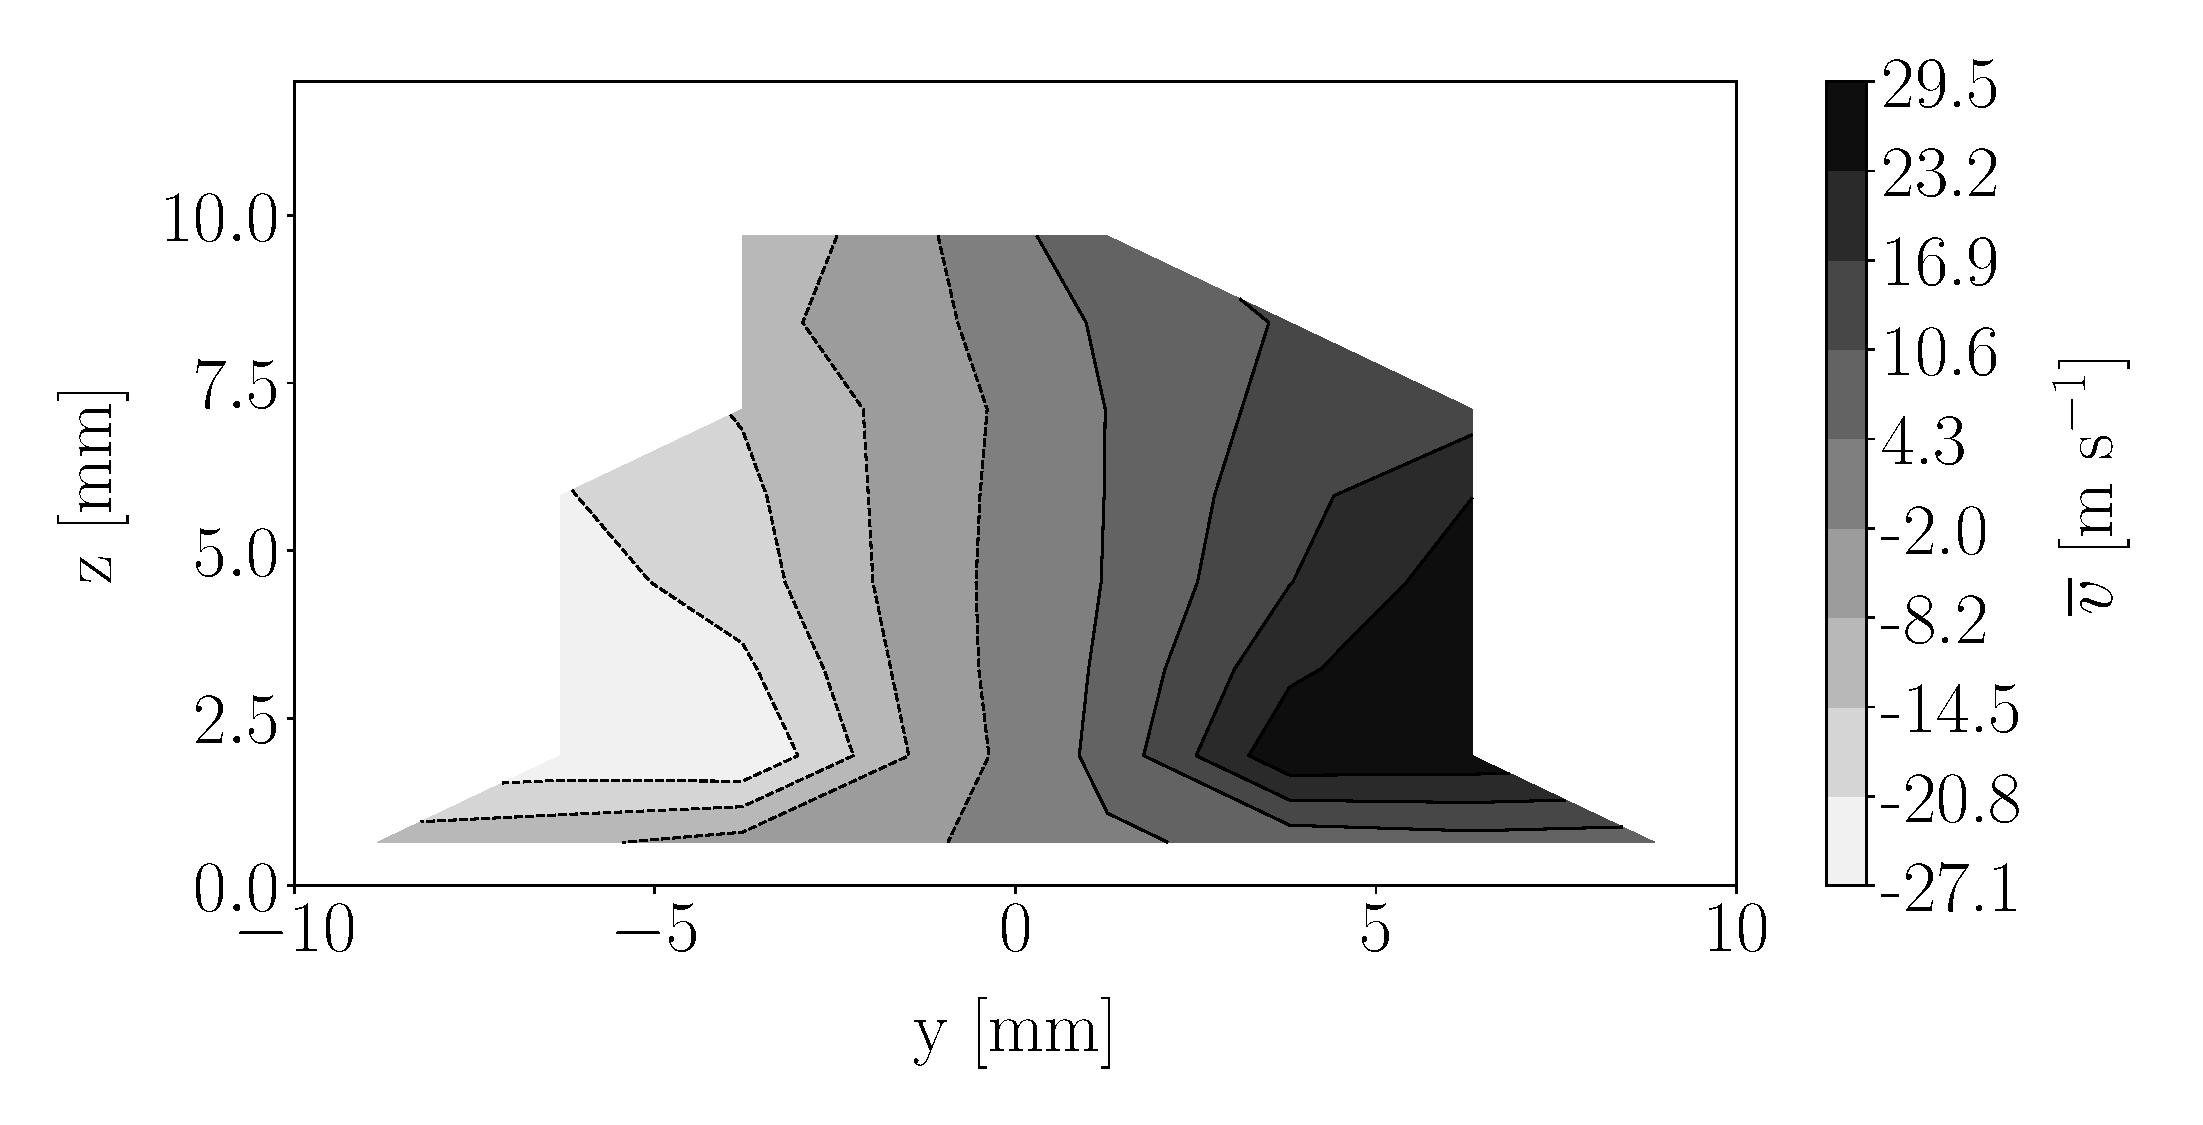
\includegraphics[scale=\scaleSLIJICF]{./part2_developments/figures_ch5_resolved_JICF/injectors_SLI/uG75_dx20_x15_uy_mean_map}
   %\caption{Case UG100\_DX20: filming planes}
   %\label{}
\end{subfigure}
   \hspace{0.17in}
\begin{subfigure}[b]{0.3\textwidth}
	\centering
   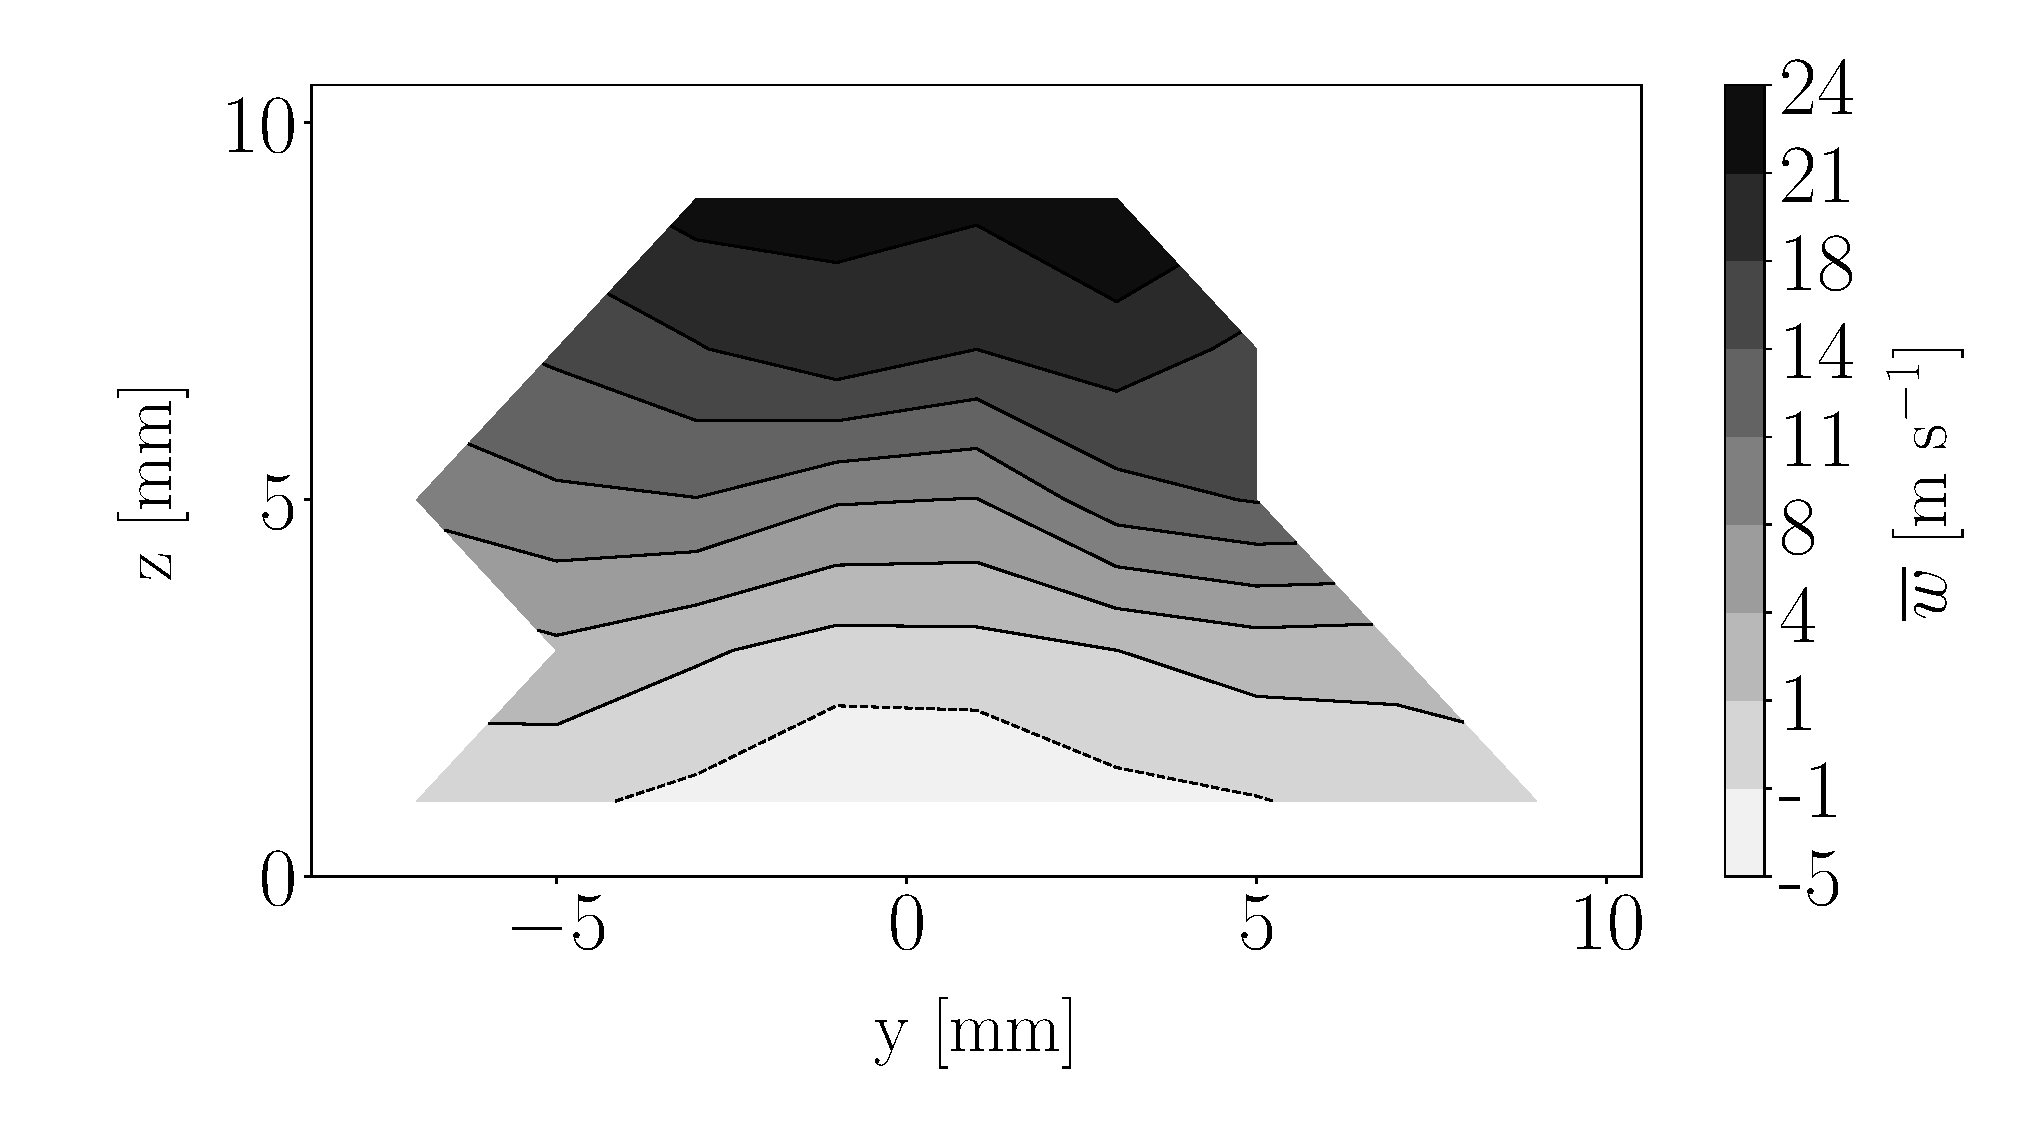
\includegraphics[scale=\scaleSLIJICF]{./part2_developments/figures_ch5_resolved_JICF/injectors_SLI/uG75_dx20_x15_uz_mean_map}
   %\caption{Case UG100\_DX10: crossflow planes}
   %\label{} 
\end{subfigure}
\caption{Spray states at x = 15 mm for case UG75\_DX20}
\label{fig:injectors_sli_uG75_dx20_x15}
\end{figure}


\clearpage

\subsubsection*{Case UG100\_DX10}



%%%%%%%%%%%%%%%% UG100_DX10, x = 5 mm


\begin{figure}[h!]
\centering
\begin{subfigure}[b]{0.3\textwidth}
	\centering
   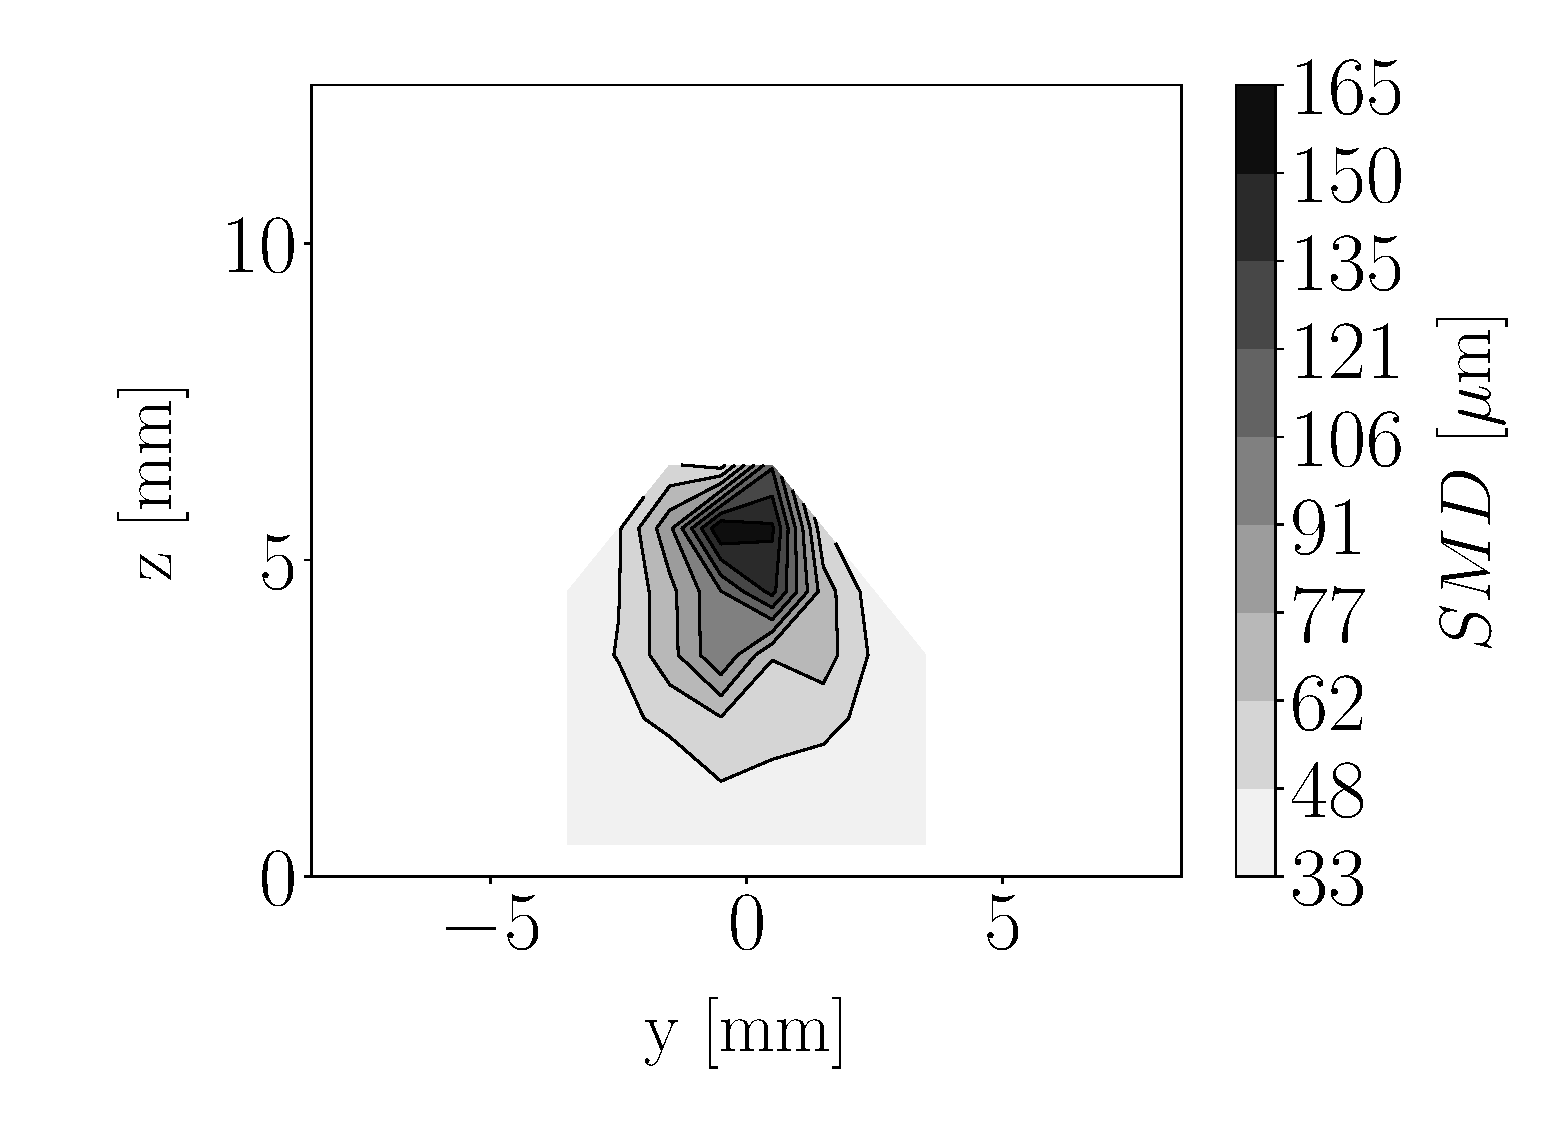
\includegraphics[scale=\scaleSLIJICF]{./part2_developments/figures_ch5_resolved_JICF/injectors_SLI/uG100_dx10_x05_SMD_map}
   %\caption{Case UG100\_DX20: crossflow planes}
   %\label{} 
\end{subfigure}
   \hspace{0.17in}
\begin{subfigure}[b]{0.3\textwidth}
	\centering
   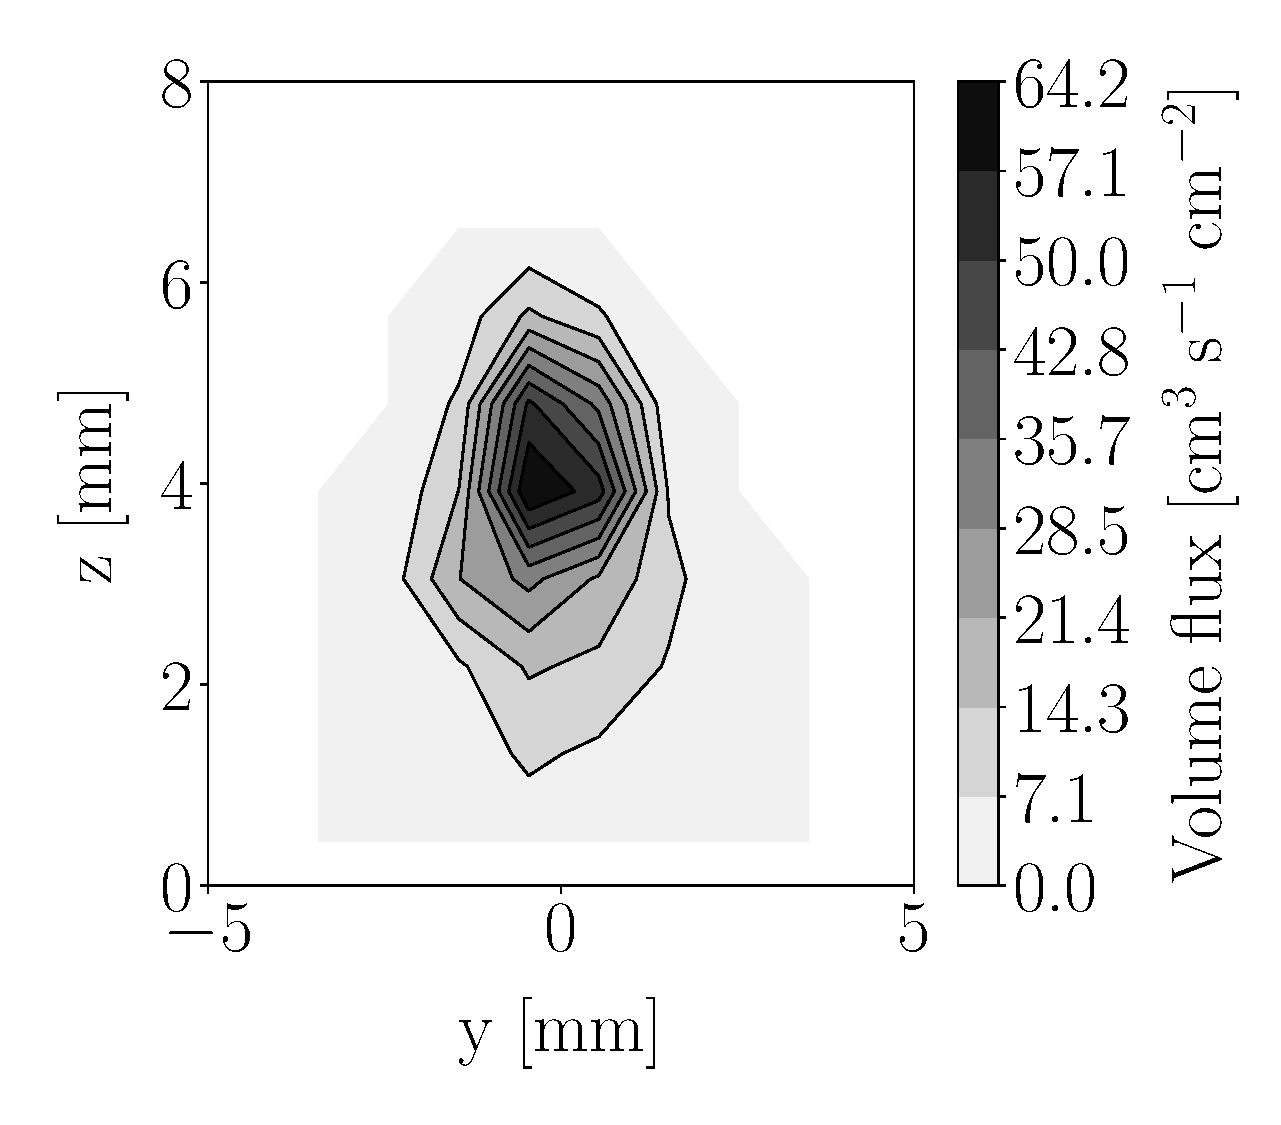
\includegraphics[scale=\scaleSLIJICF]{./part2_developments/figures_ch5_resolved_JICF/injectors_SLI/uG100_dx10_x05_volume_flux_map}
   %\caption{Case UG100\_DX20: filming planes}
   %\label{}
\end{subfigure}
   \hspace{0.17in}
\begin{subfigure}[b]{0.3\textwidth}
	\centering
   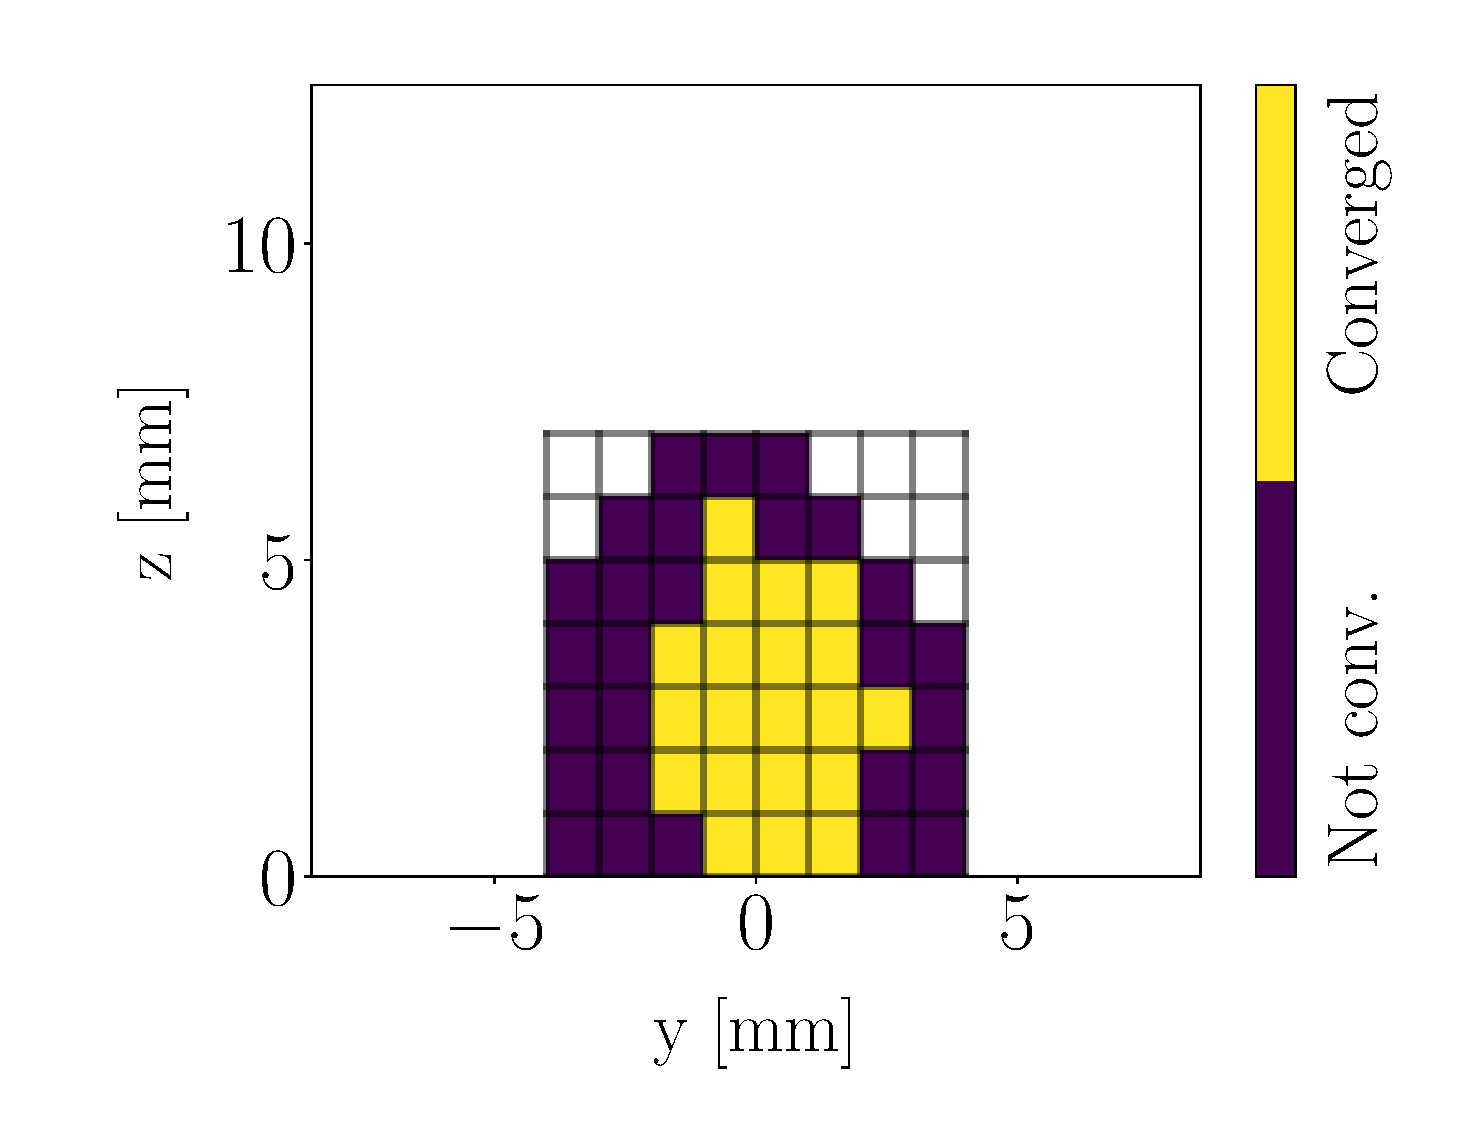
\includegraphics[scale=\scaleSLIJICF]{./part2_developments/figures_ch5_resolved_JICF/injectors_SLI/uG100_dx10_x05_convergence_map}
   %\caption{Case UG100\_DX10: crossflow planes}
   %\label{} 
\end{subfigure}

\vskip\baselineskip

\begin{subfigure}[b]{0.3\textwidth}
	\centering
   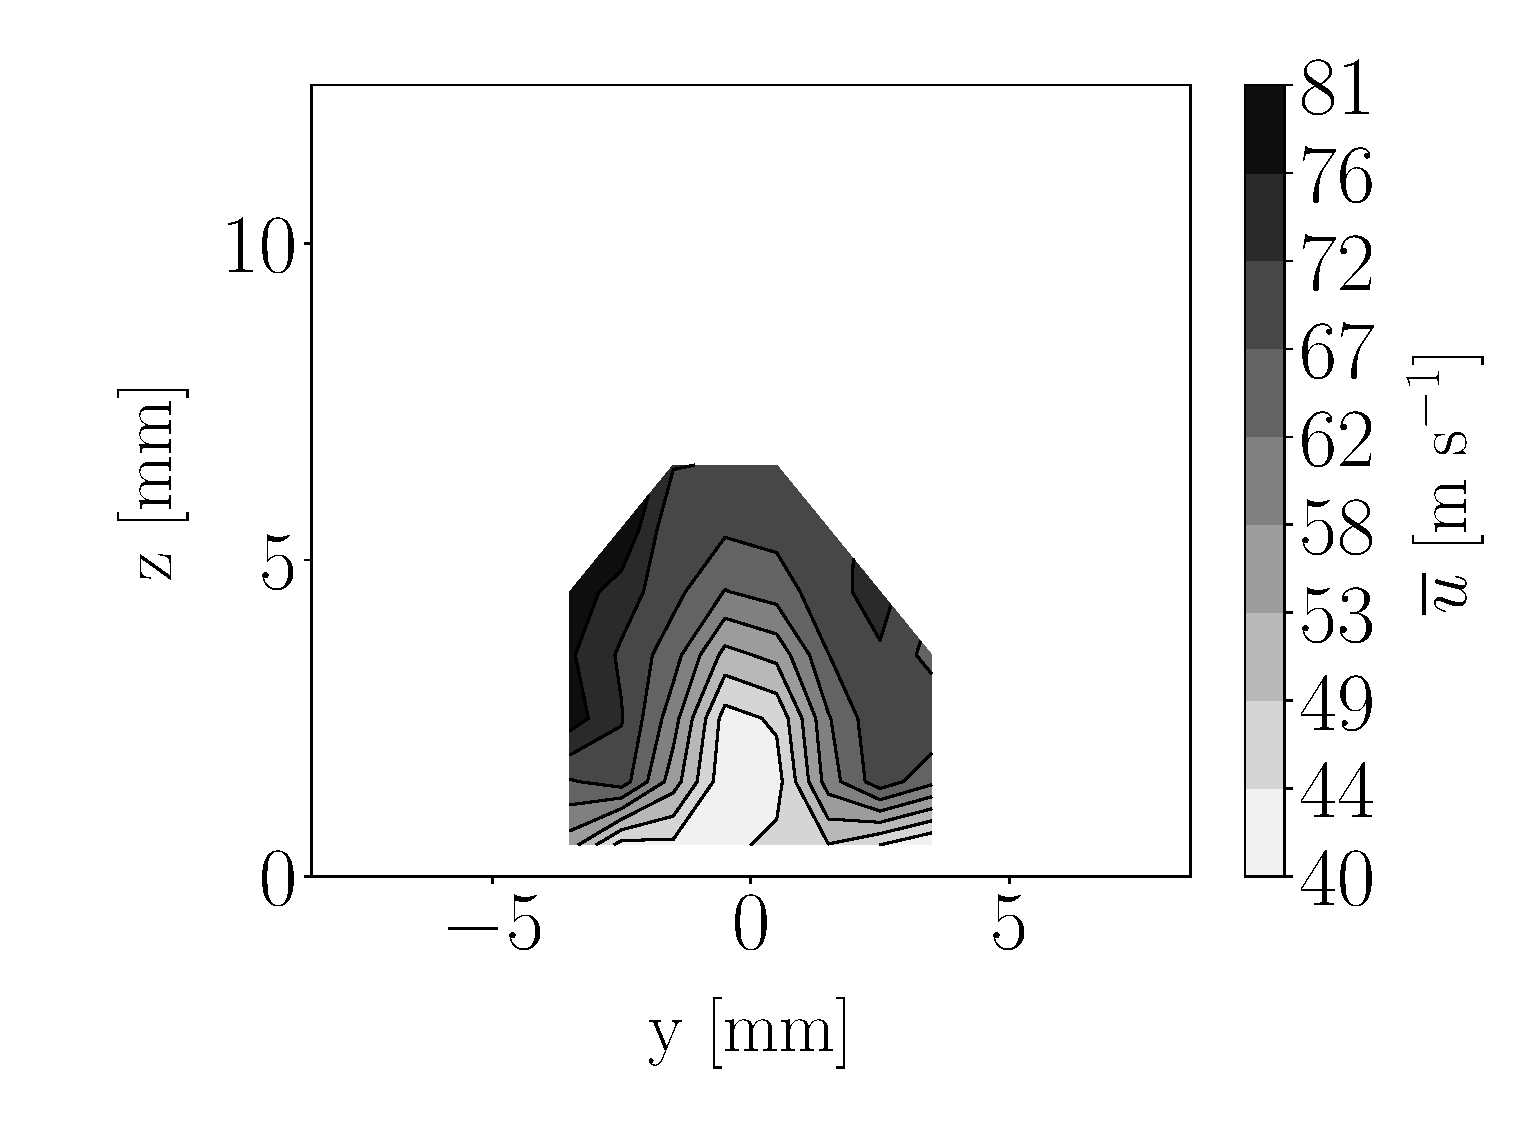
\includegraphics[scale=\scaleSLIJICF]{./part2_developments/figures_ch5_resolved_JICF/injectors_SLI/uG100_dx10_x05_ux_mean_map}
   %\caption{Case UG100\_DX20: crossflow planes}
   %\label{} 
\end{subfigure}
   \hspace{0.17in}
\begin{subfigure}[b]{0.3\textwidth}
	\centering
   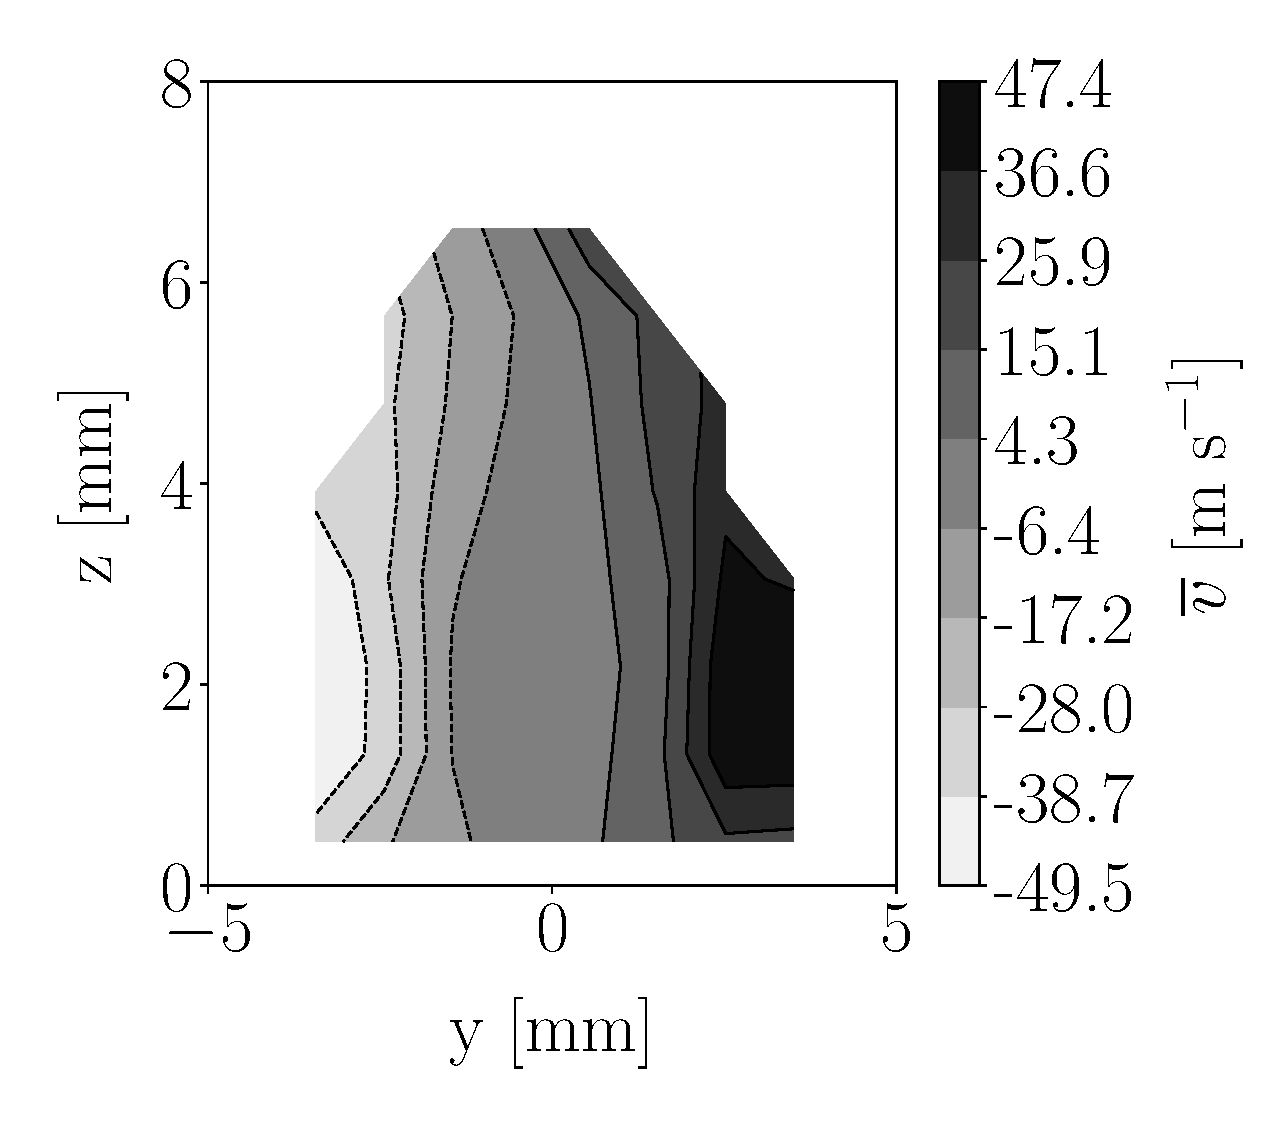
\includegraphics[scale=\scaleSLIJICF]{./part2_developments/figures_ch5_resolved_JICF/injectors_SLI/uG100_dx10_x05_uy_mean_map}
   %\caption{Case UG100\_DX20: filming planes}
   %\label{}
\end{subfigure}
   \hspace{0.17in}
\begin{subfigure}[b]{0.3\textwidth}
	\centering
   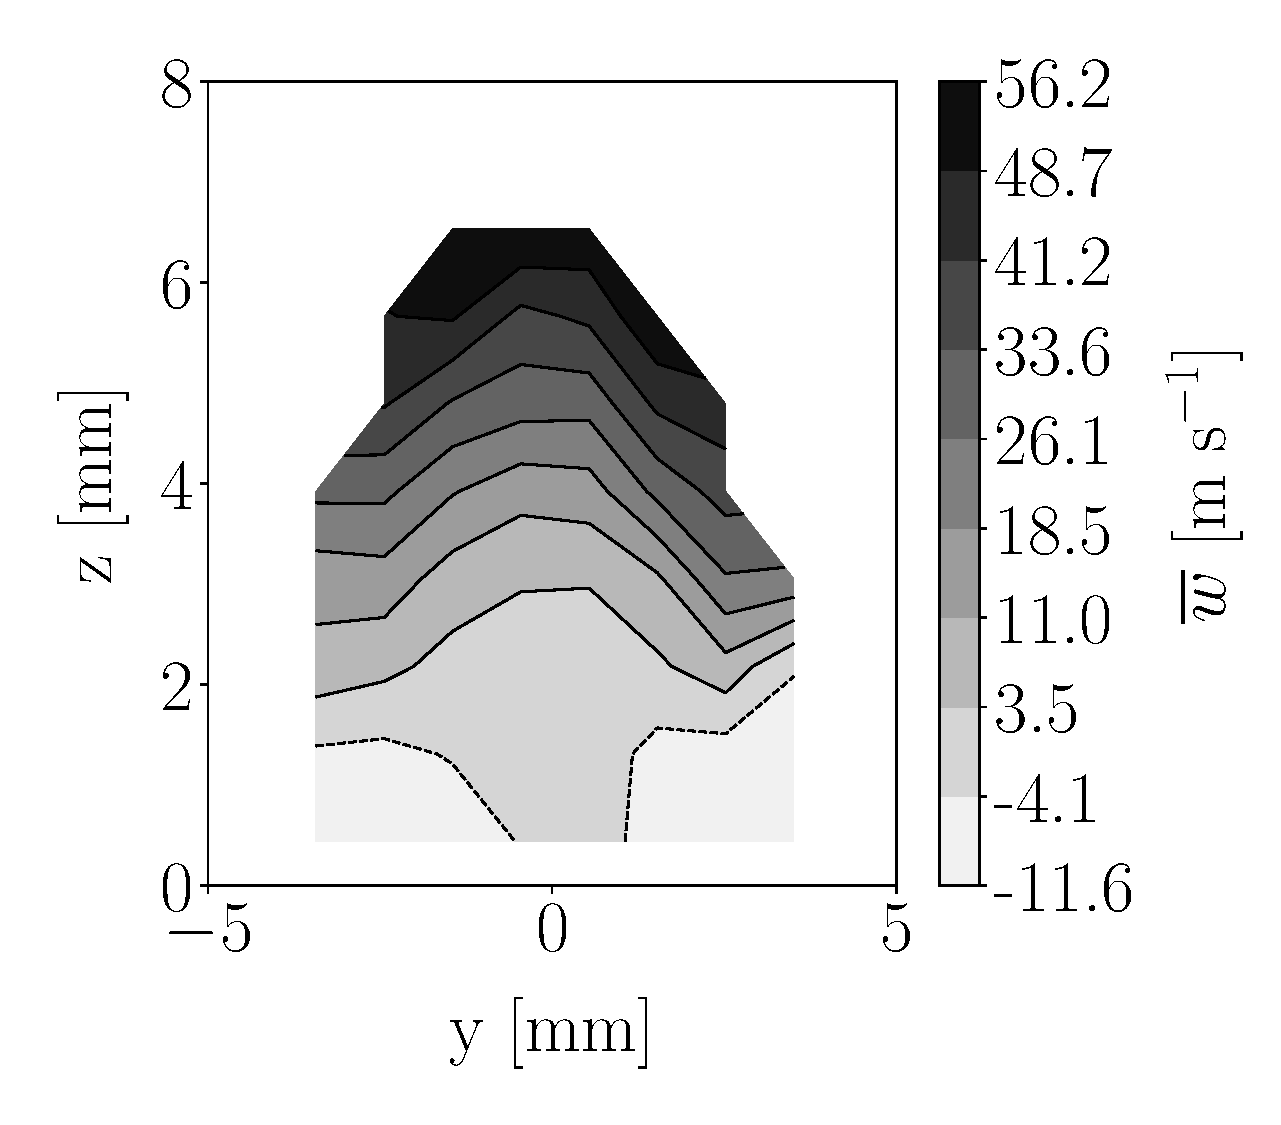
\includegraphics[scale=\scaleSLIJICF]{./part2_developments/figures_ch5_resolved_JICF/injectors_SLI/uG100_dx10_x05_uz_mean_map}
   %\caption{Case UG100\_DX10: crossflow planes}
   %\label{} 
\end{subfigure}
\caption{Spray states at x = 5 mm for case UG100\_DX10}
\label{fig:injectors_sli_uG100_dx10_x05}
\end{figure}


%%%%%%%%%%%%%%%% UG100_DX10, x = 10 mm


\begin{figure}[h!]
\centering\begin{subfigure}[b]{0.3\textwidth}
	\centering
   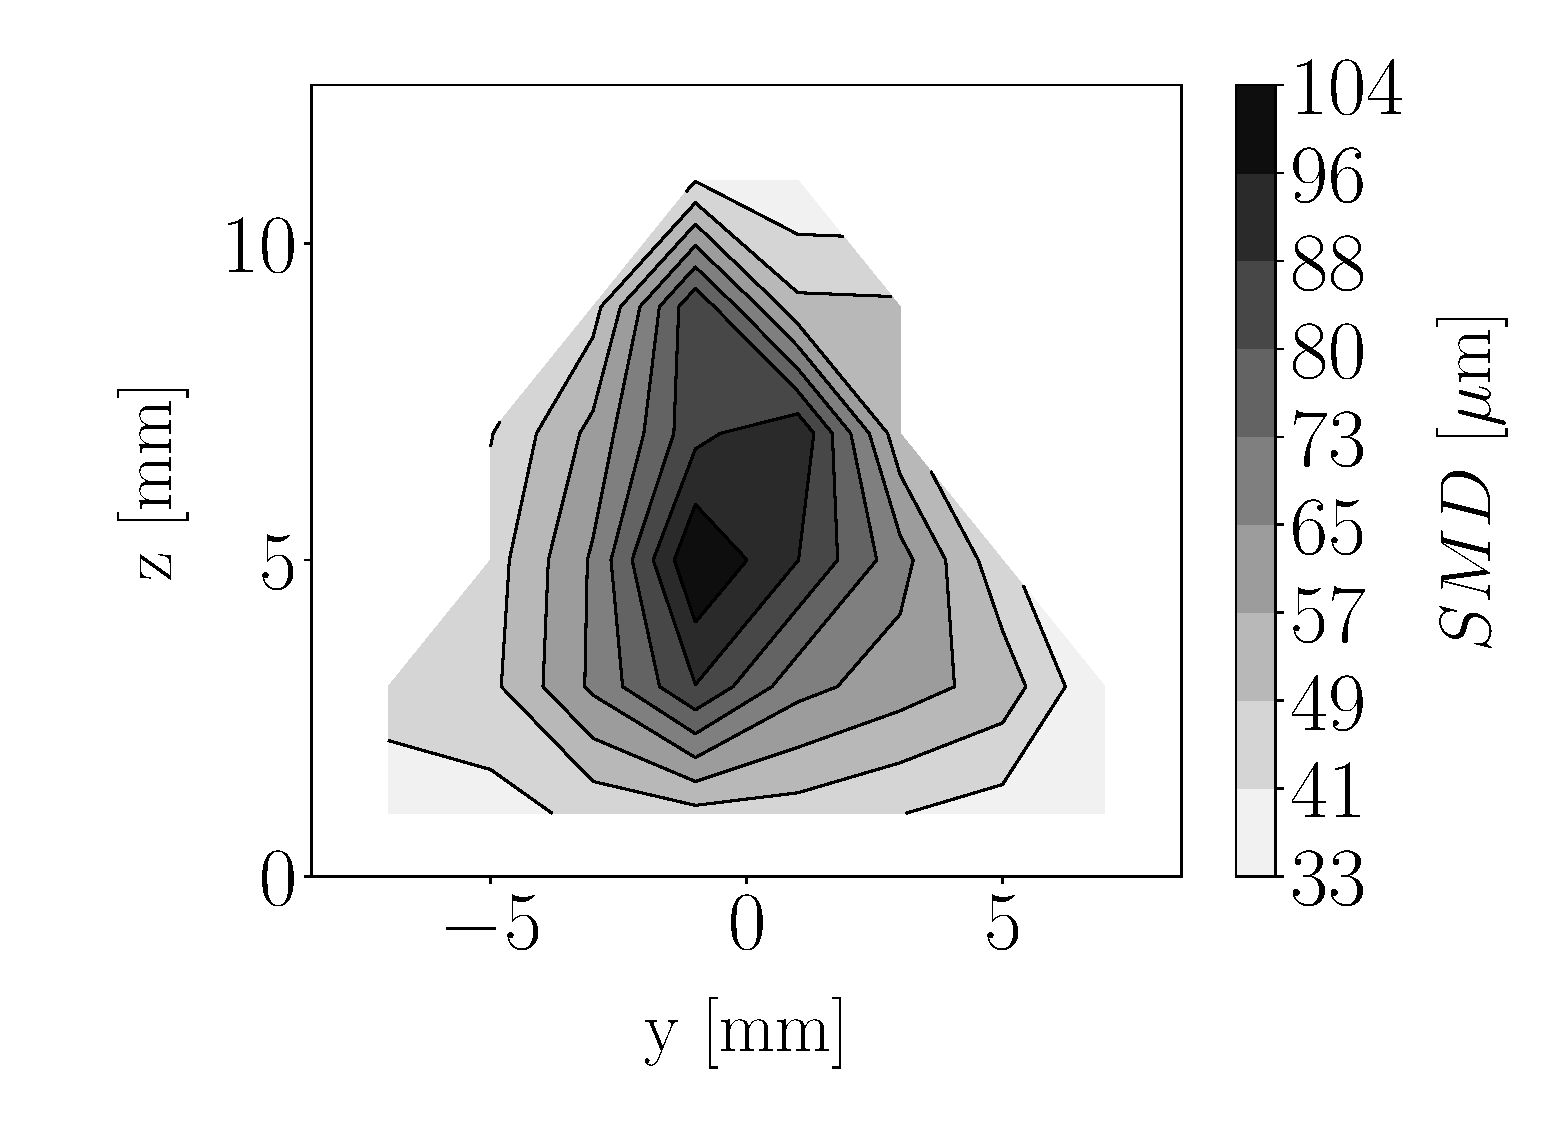
\includegraphics[scale=\scaleSLIJICF]{./part2_developments/figures_ch5_resolved_JICF/injectors_SLI/uG100_dx10_x10_SMD_map}
   %\caption{Case UG100\_DX20: crossflow planes}
   %\label{} 
\end{subfigure}
   \hspace{0.17in}
\begin{subfigure}[b]{0.3\textwidth}
	\centering
   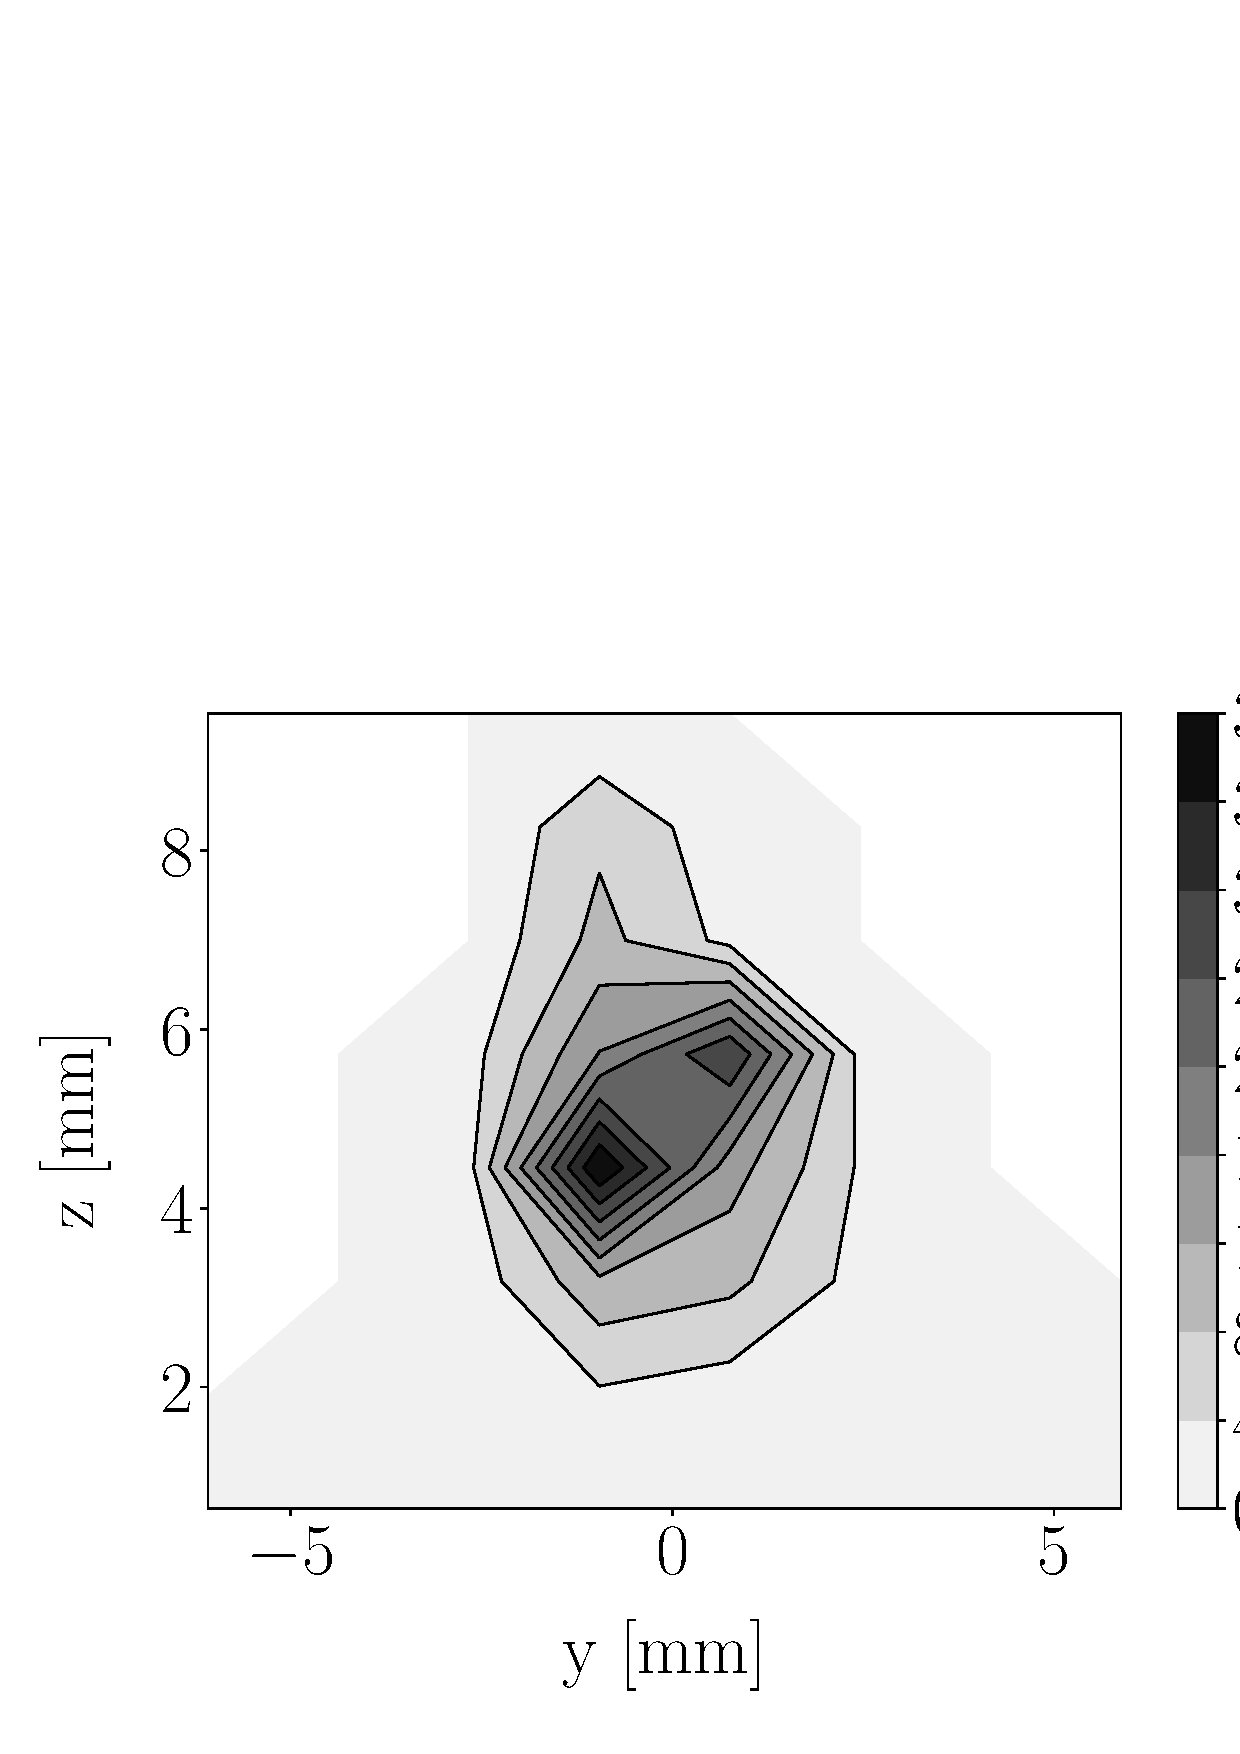
\includegraphics[scale=\scaleSLIJICF]{./part2_developments/figures_ch5_resolved_JICF/injectors_SLI/uG100_dx10_x10_volume_flux_map}
   %\caption{Case UG100\_DX20: filming planes}
   %\label{}
\end{subfigure}
   \hspace{0.17in}
\begin{subfigure}[b]{0.3\textwidth}
	\centering
   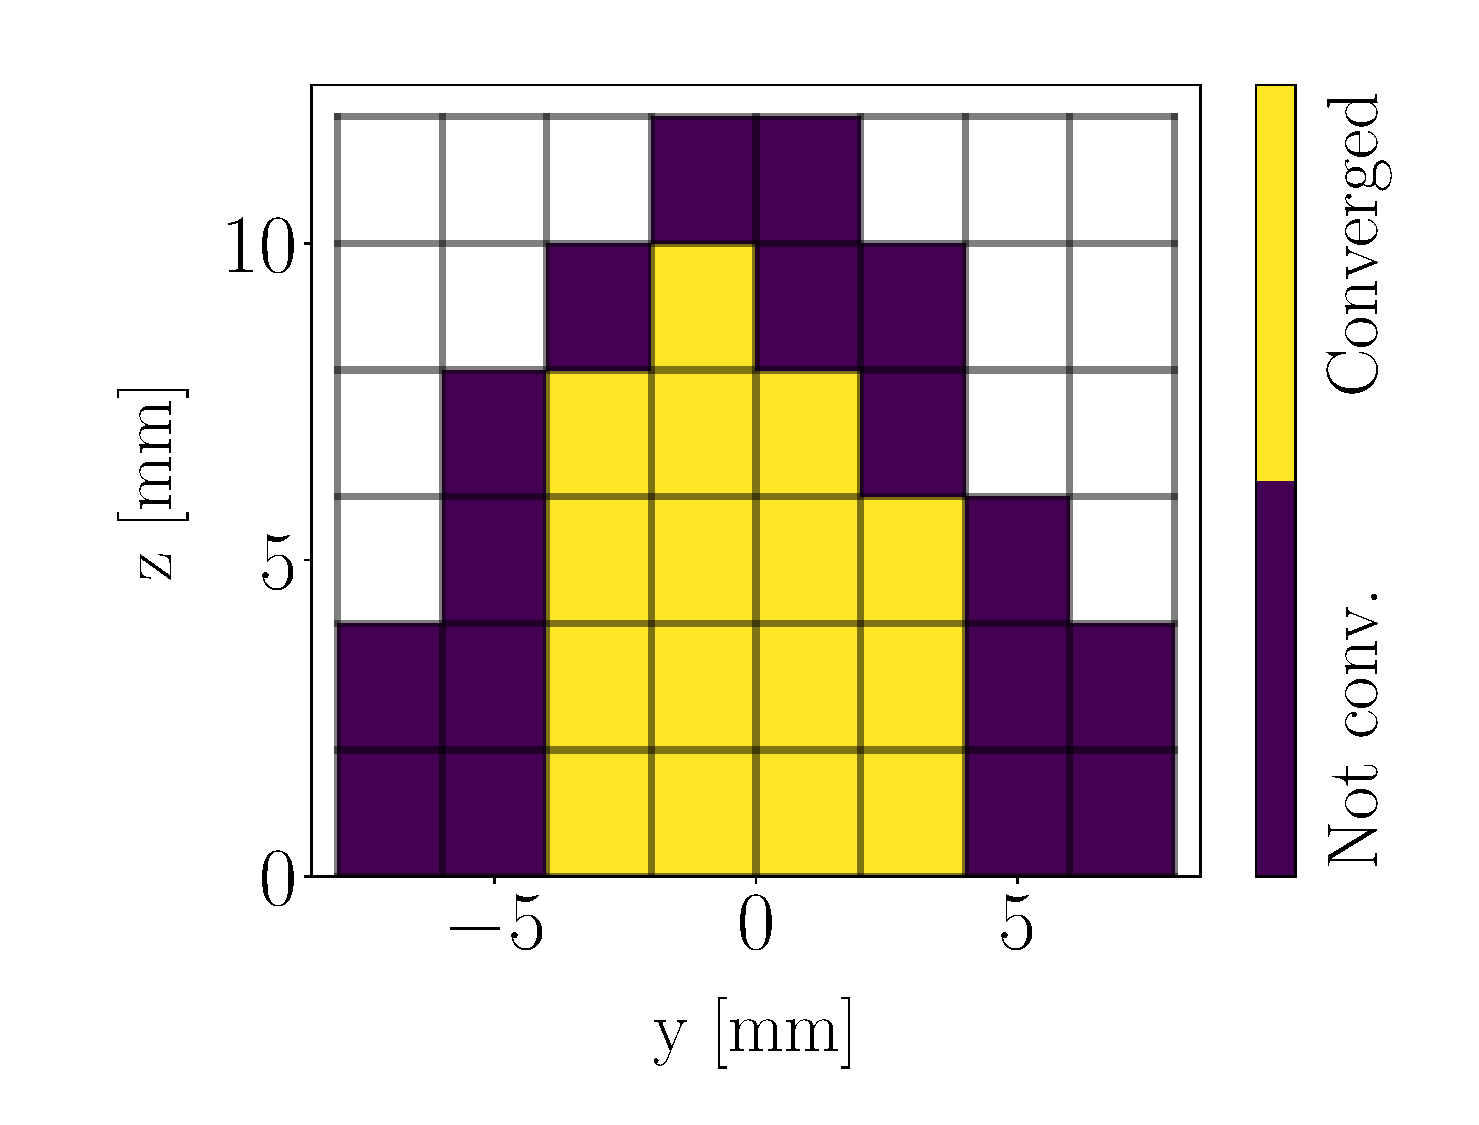
\includegraphics[scale=\scaleSLIJICF]{./part2_developments/figures_ch5_resolved_JICF/injectors_SLI/uG100_dx10_x10_convergence_map}
   %\caption{Case UG100\_DX10: crossflow planes}
   %\label{} 
\end{subfigure}

\vskip\baselineskip

\begin{subfigure}[b]{0.3\textwidth}
	\centering
   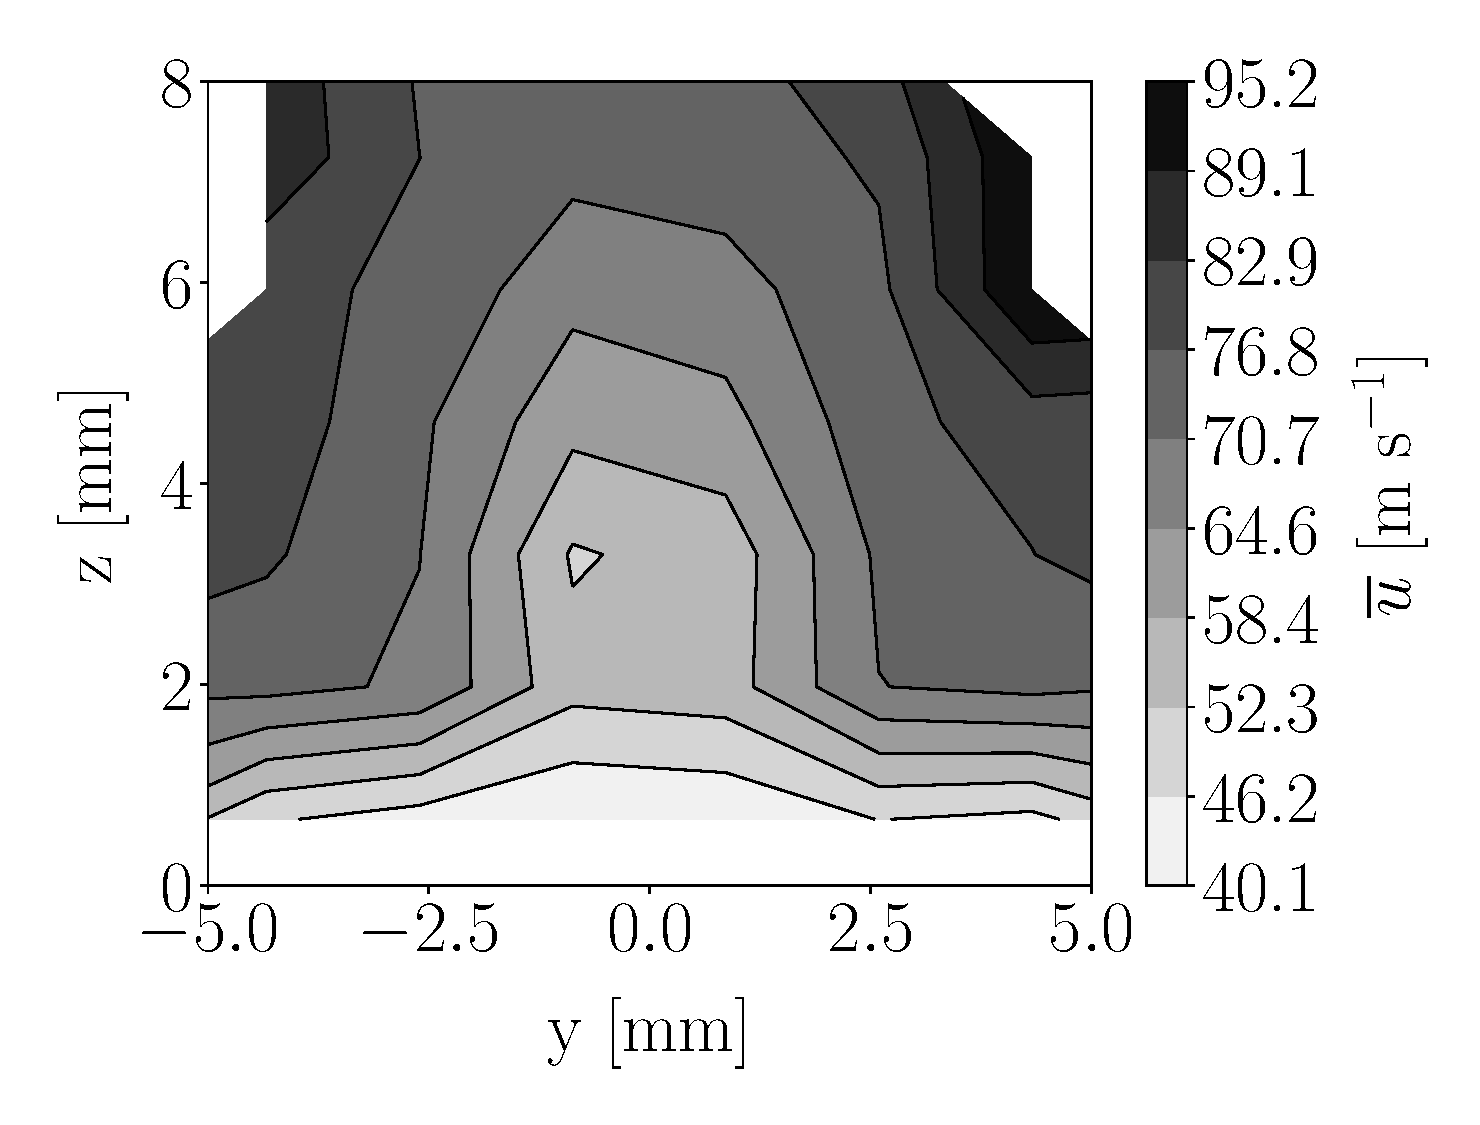
\includegraphics[scale=\scaleSLIJICF]{./part2_developments/figures_ch5_resolved_JICF/injectors_SLI/uG100_dx10_x10_ux_mean_map}
   %\caption{Case UG100\_DX20: crossflow planes}
   %\label{} 
\end{subfigure}
   \hspace{0.17in}
\begin{subfigure}[b]{0.3\textwidth}
	\centering
   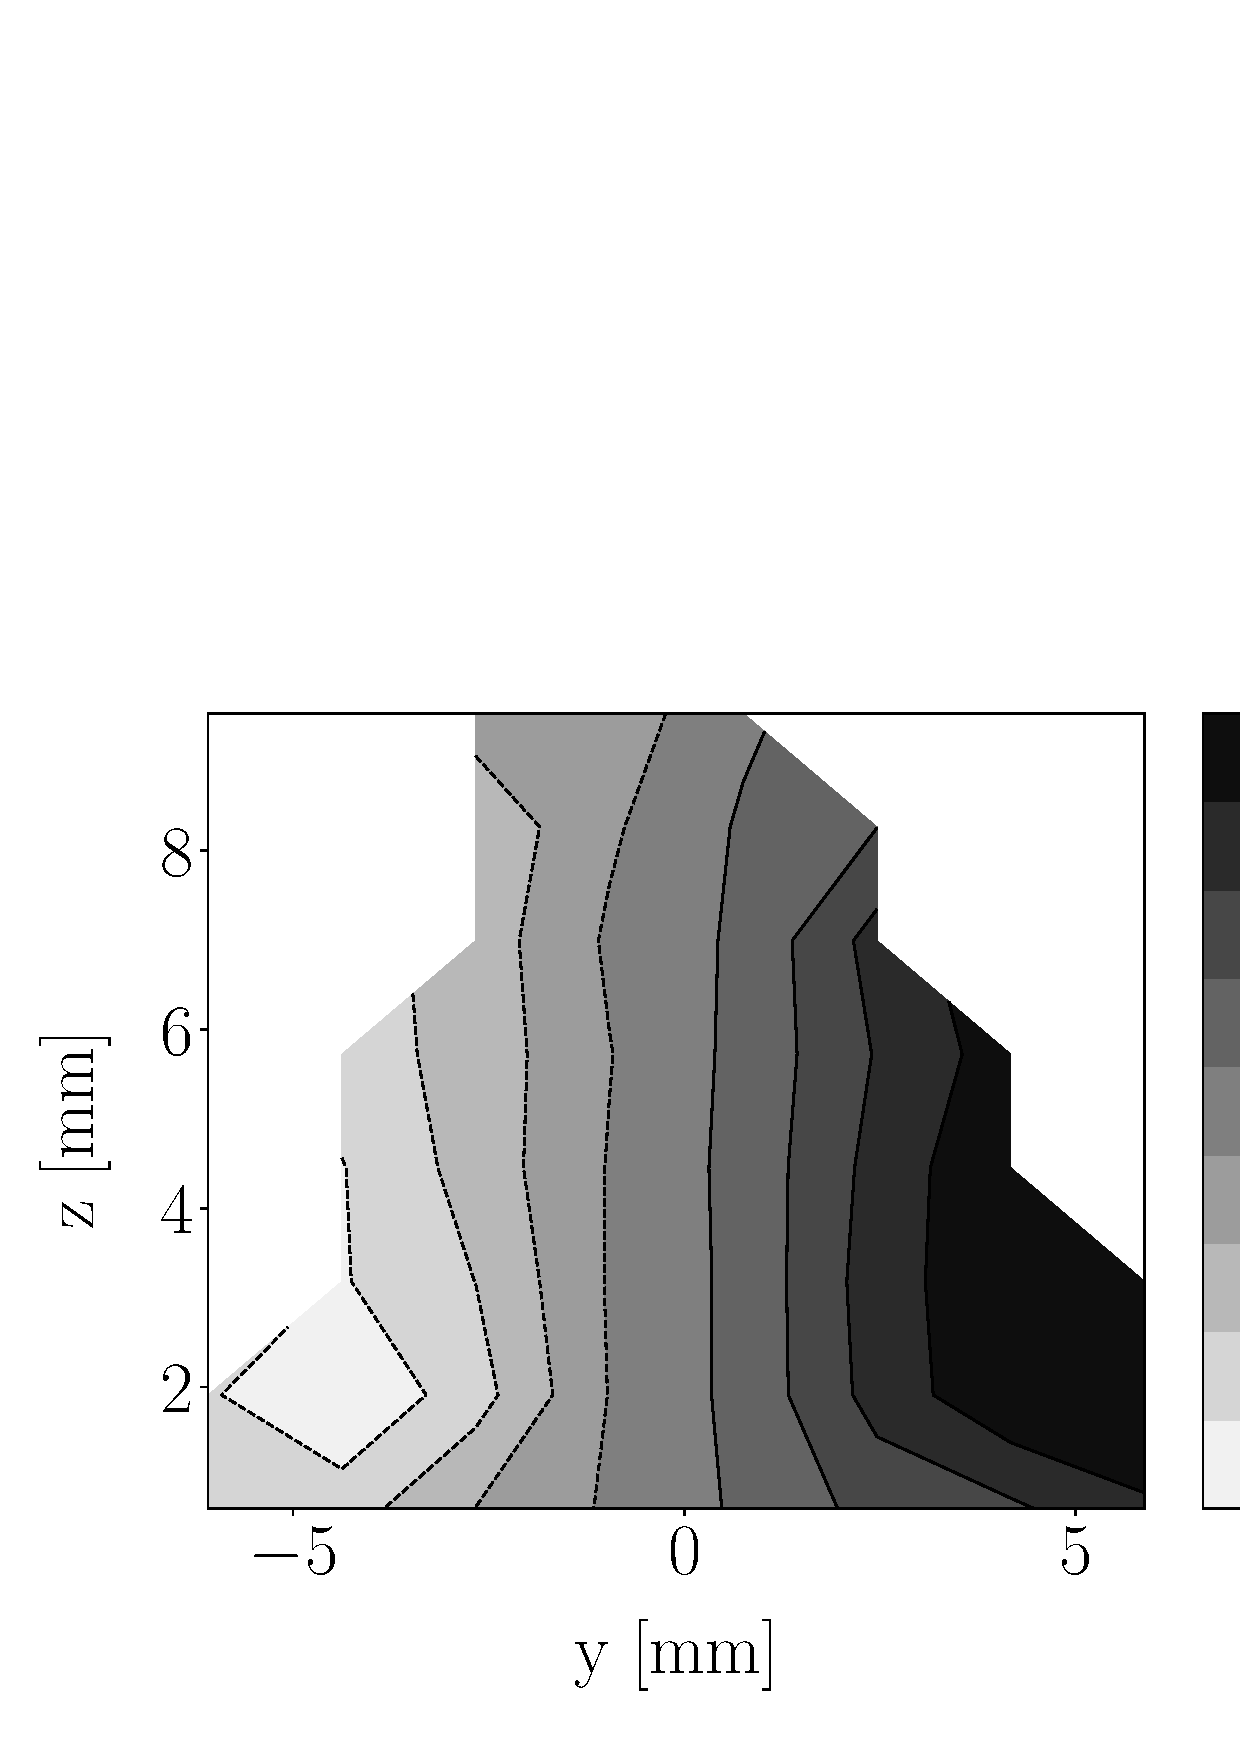
\includegraphics[scale=\scaleSLIJICF]{./part2_developments/figures_ch5_resolved_JICF/injectors_SLI/uG100_dx10_x10_uy_mean_map}
   %\caption{Case UG100\_DX20: filming planes}
   %\label{}
\end{subfigure}
   \hspace{0.17in}
\begin{subfigure}[b]{0.3\textwidth}
	\centering
   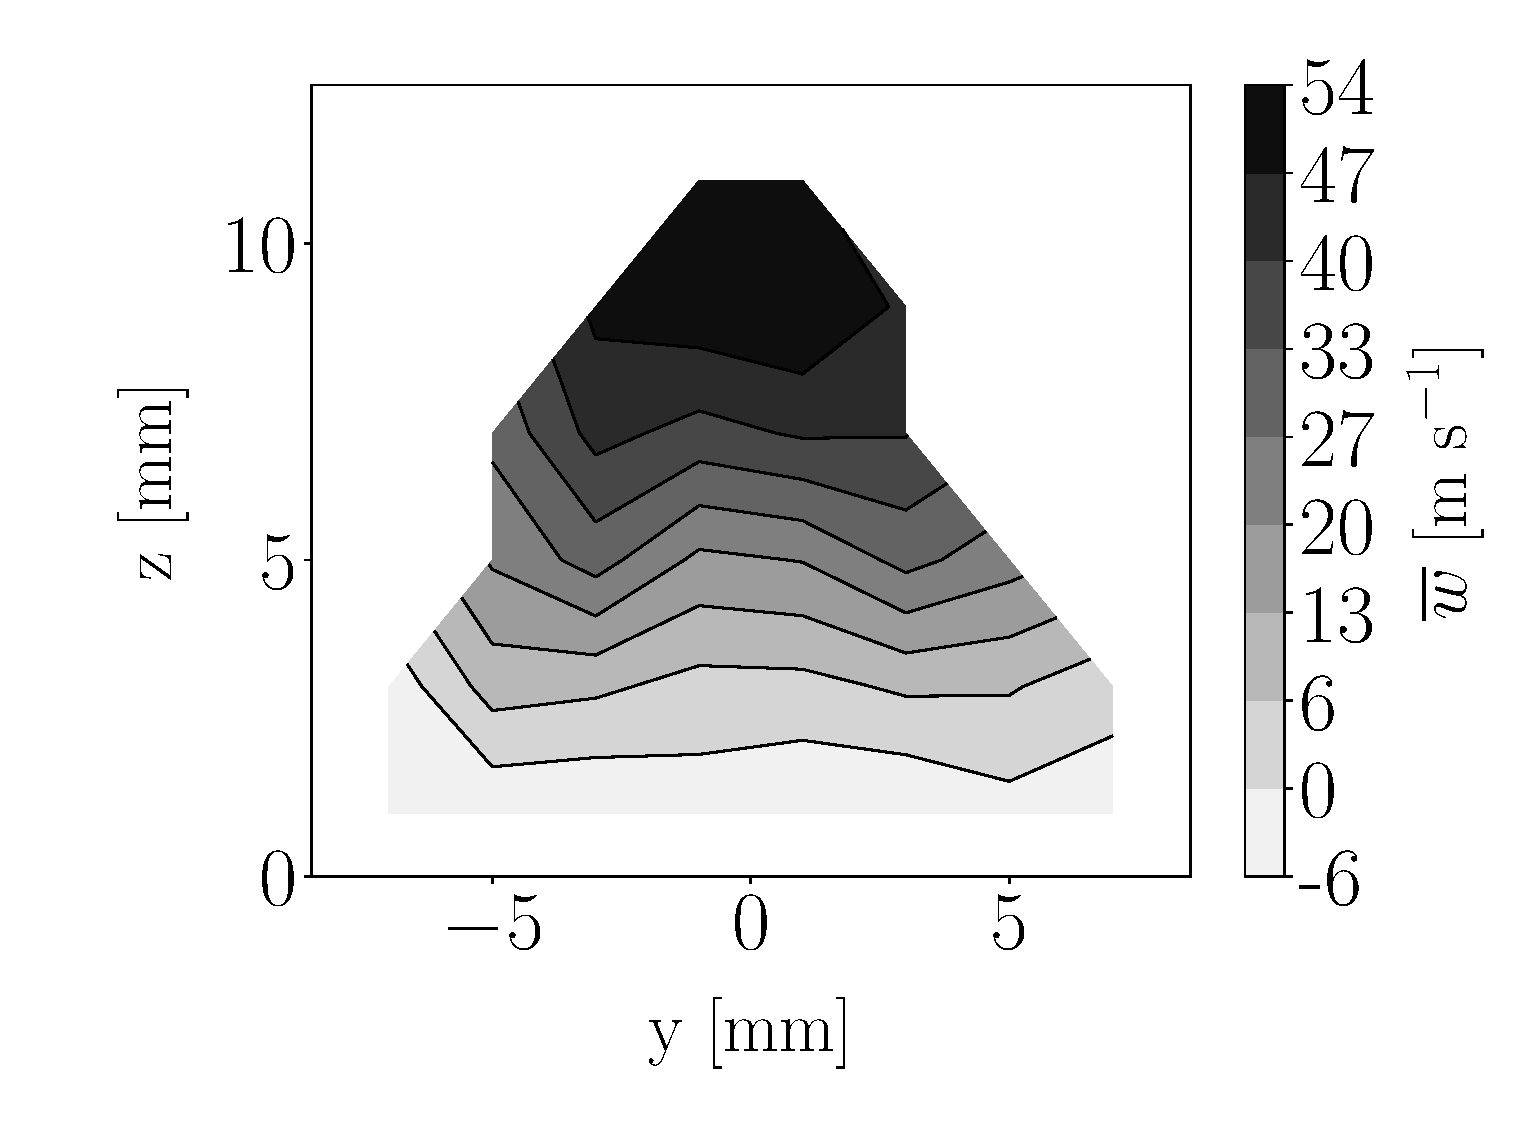
\includegraphics[scale=\scaleSLIJICF]{./part2_developments/figures_ch5_resolved_JICF/injectors_SLI/uG100_dx10_x10_uz_mean_map}
   %\caption{Case UG100\_DX10: crossflow planes}
   %\label{} 
\end{subfigure}
\caption{Spray states at x = 10 mm for case UG100\_DX10}
\label{fig:injectors_sli_uG100_dx10_x10}
\end{figure}


\clearpage

\subsubsection*{Case UG100\_DX20}



%%%%%%%%%%%%%%%% UG100_DX20, x = 5 mm


\begin{figure}[h!]
\centering
\begin{subfigure}[b]{0.3\textwidth}
	\centering
   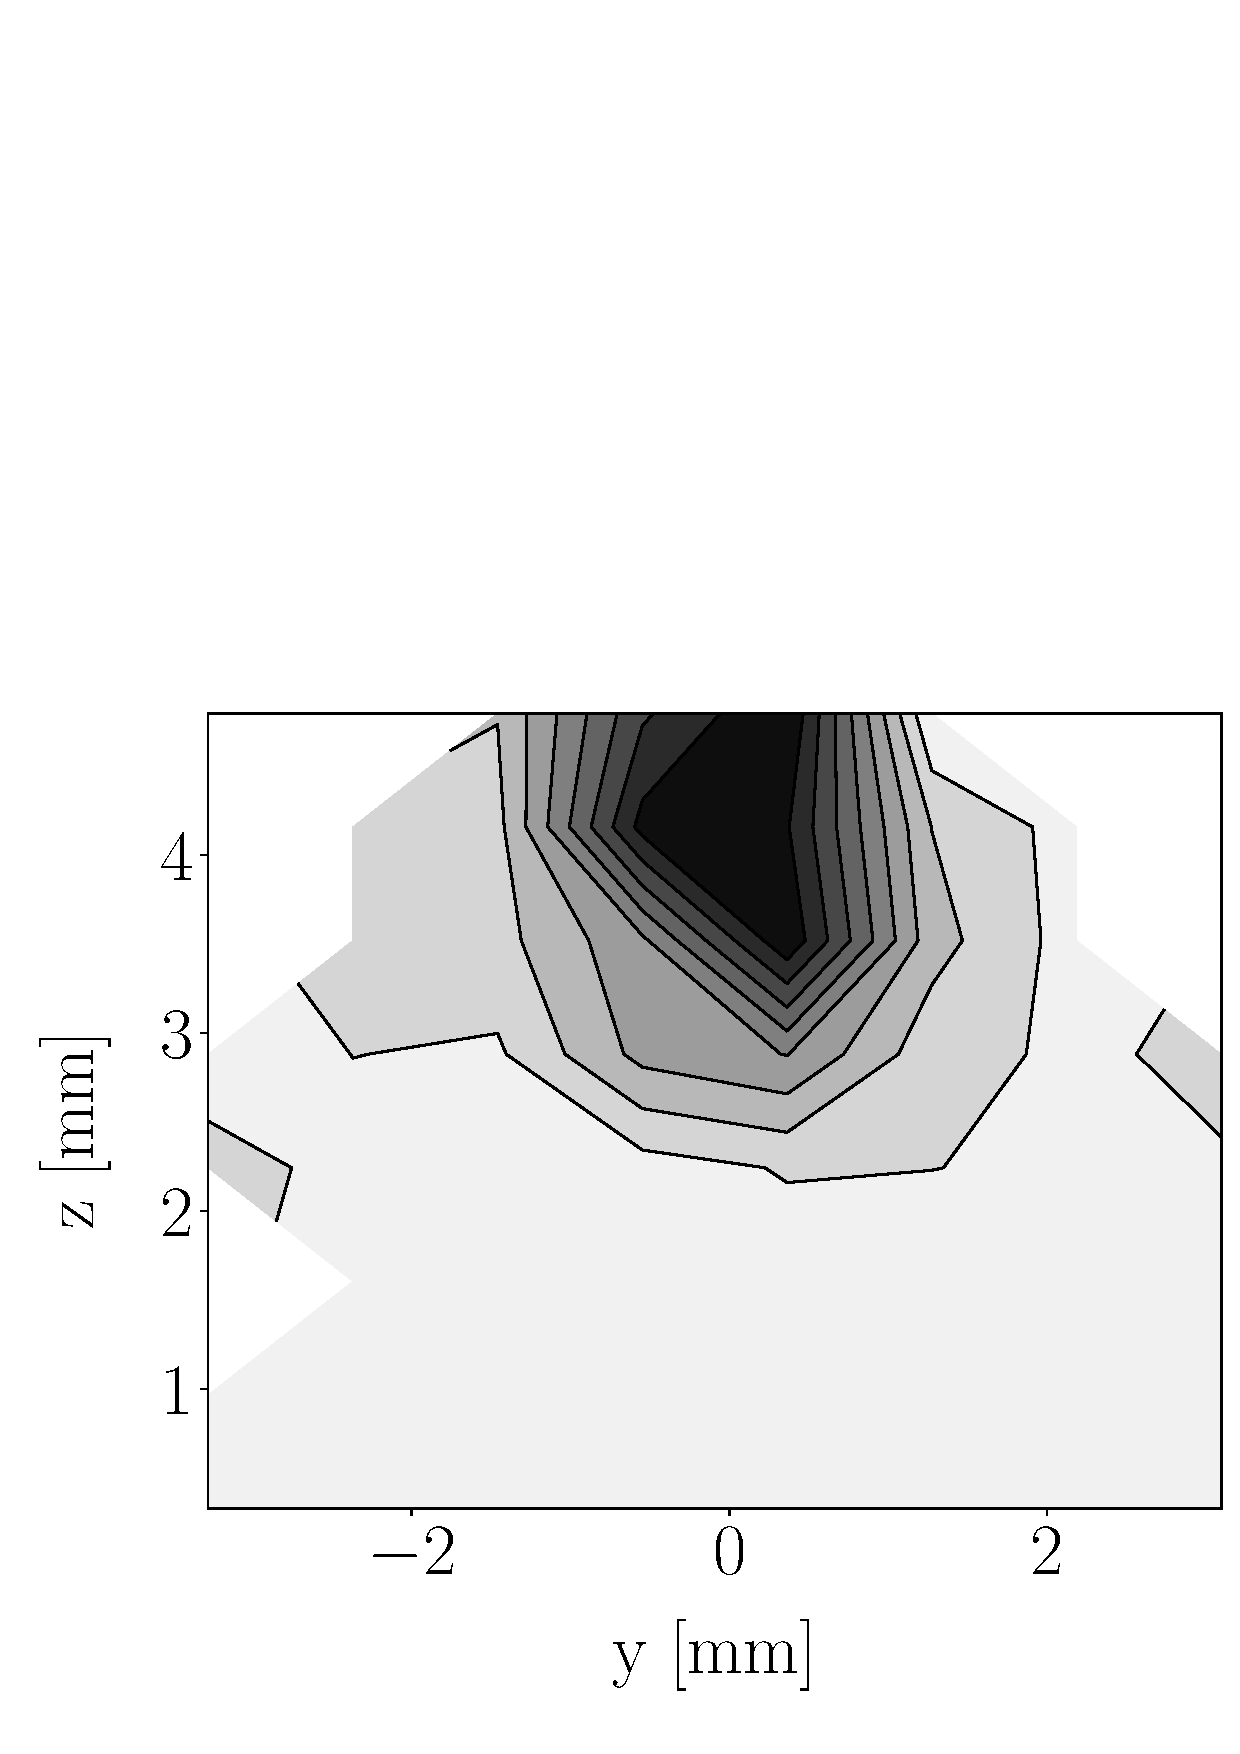
\includegraphics[scale=\scaleSLIJICF]{./part2_developments/figures_ch5_resolved_JICF/injectors_SLI/uG100_dx20_x05_SMD_map}
   %\caption{Case UG100\_DX20: crossflow planes}
   %\label{} 
\end{subfigure}
   \hspace{0.17in}
\begin{subfigure}[b]{0.3\textwidth}
	\centering
   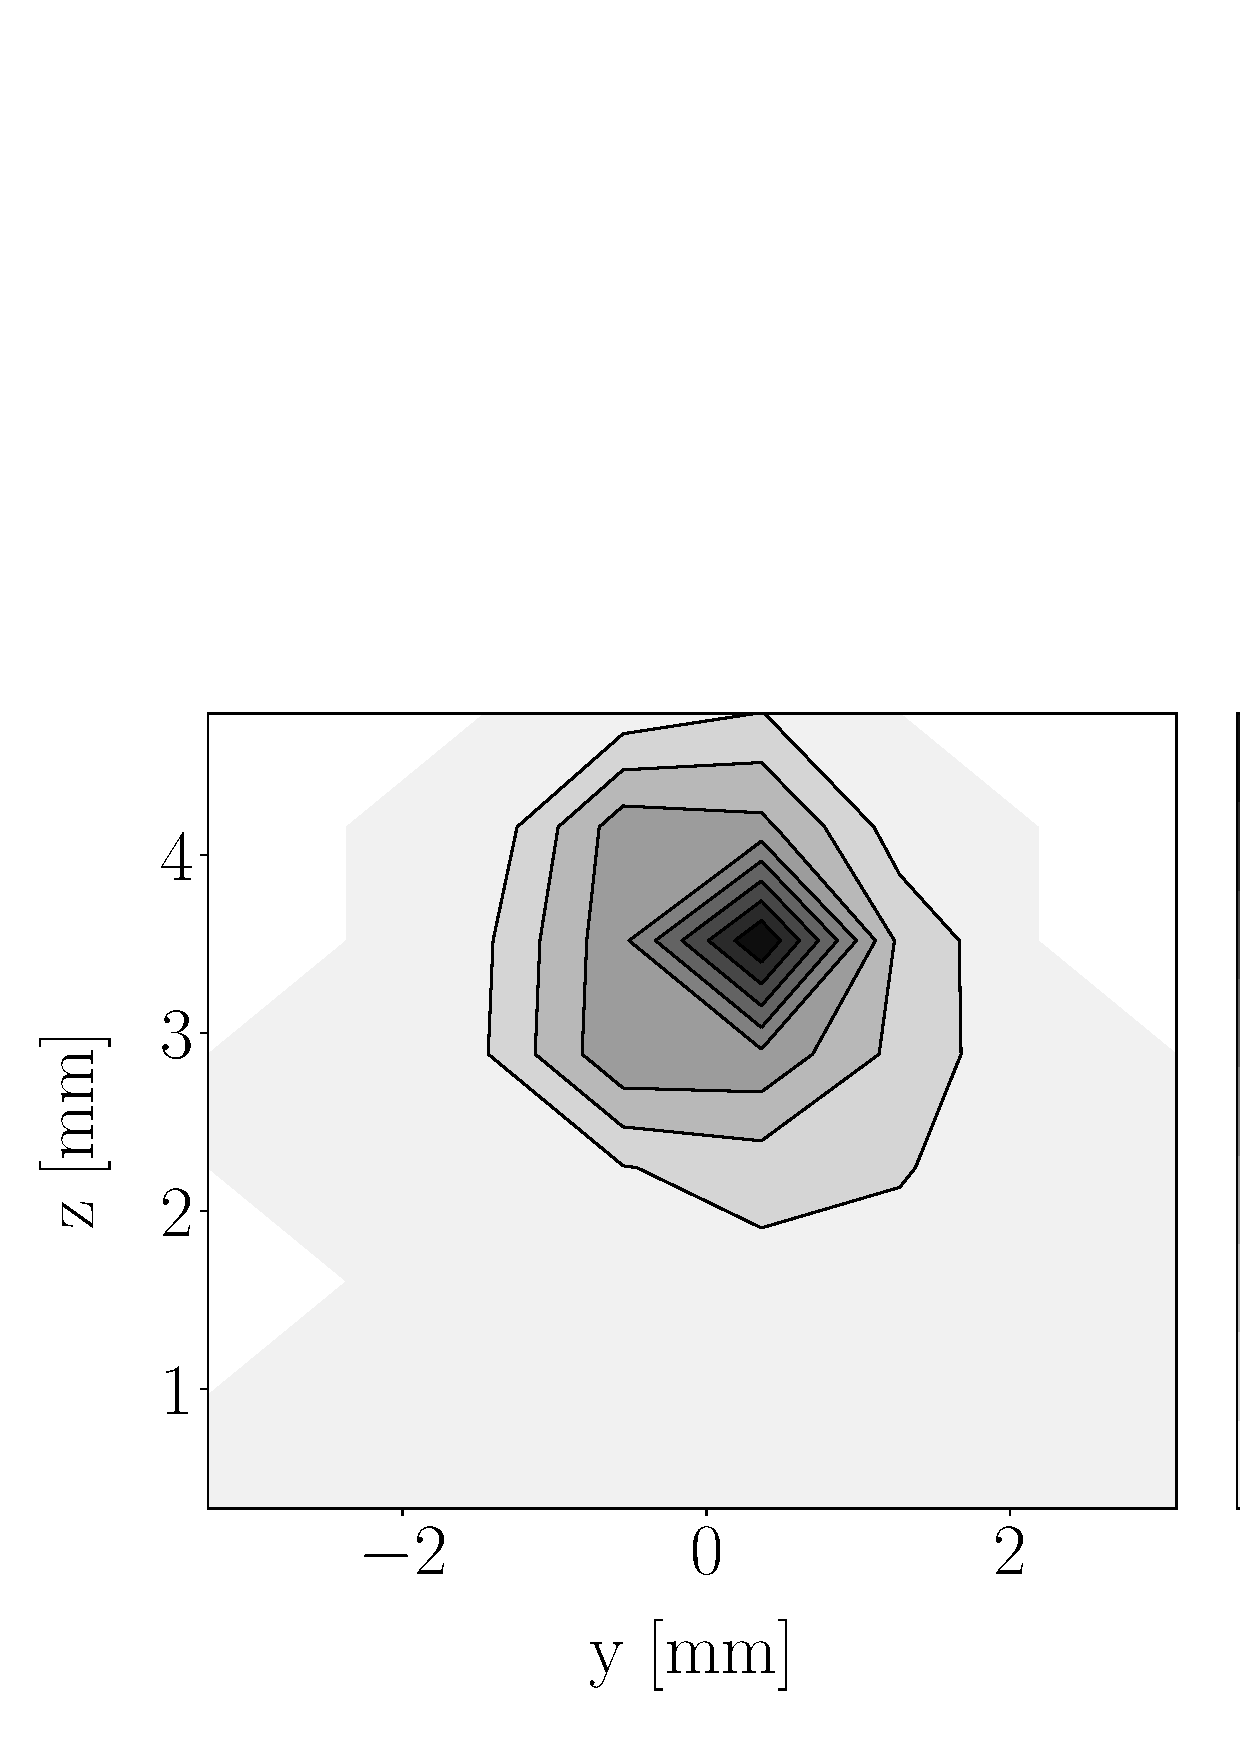
\includegraphics[scale=\scaleSLIJICF]{./part2_developments/figures_ch5_resolved_JICF/injectors_SLI/uG100_dx20_x05_volume_flux_map}
   %\caption{Case UG100\_DX20: filming planes}
   %\label{}
\end{subfigure}
   \hspace{0.17in}
\begin{subfigure}[b]{0.3\textwidth}
	\centering
   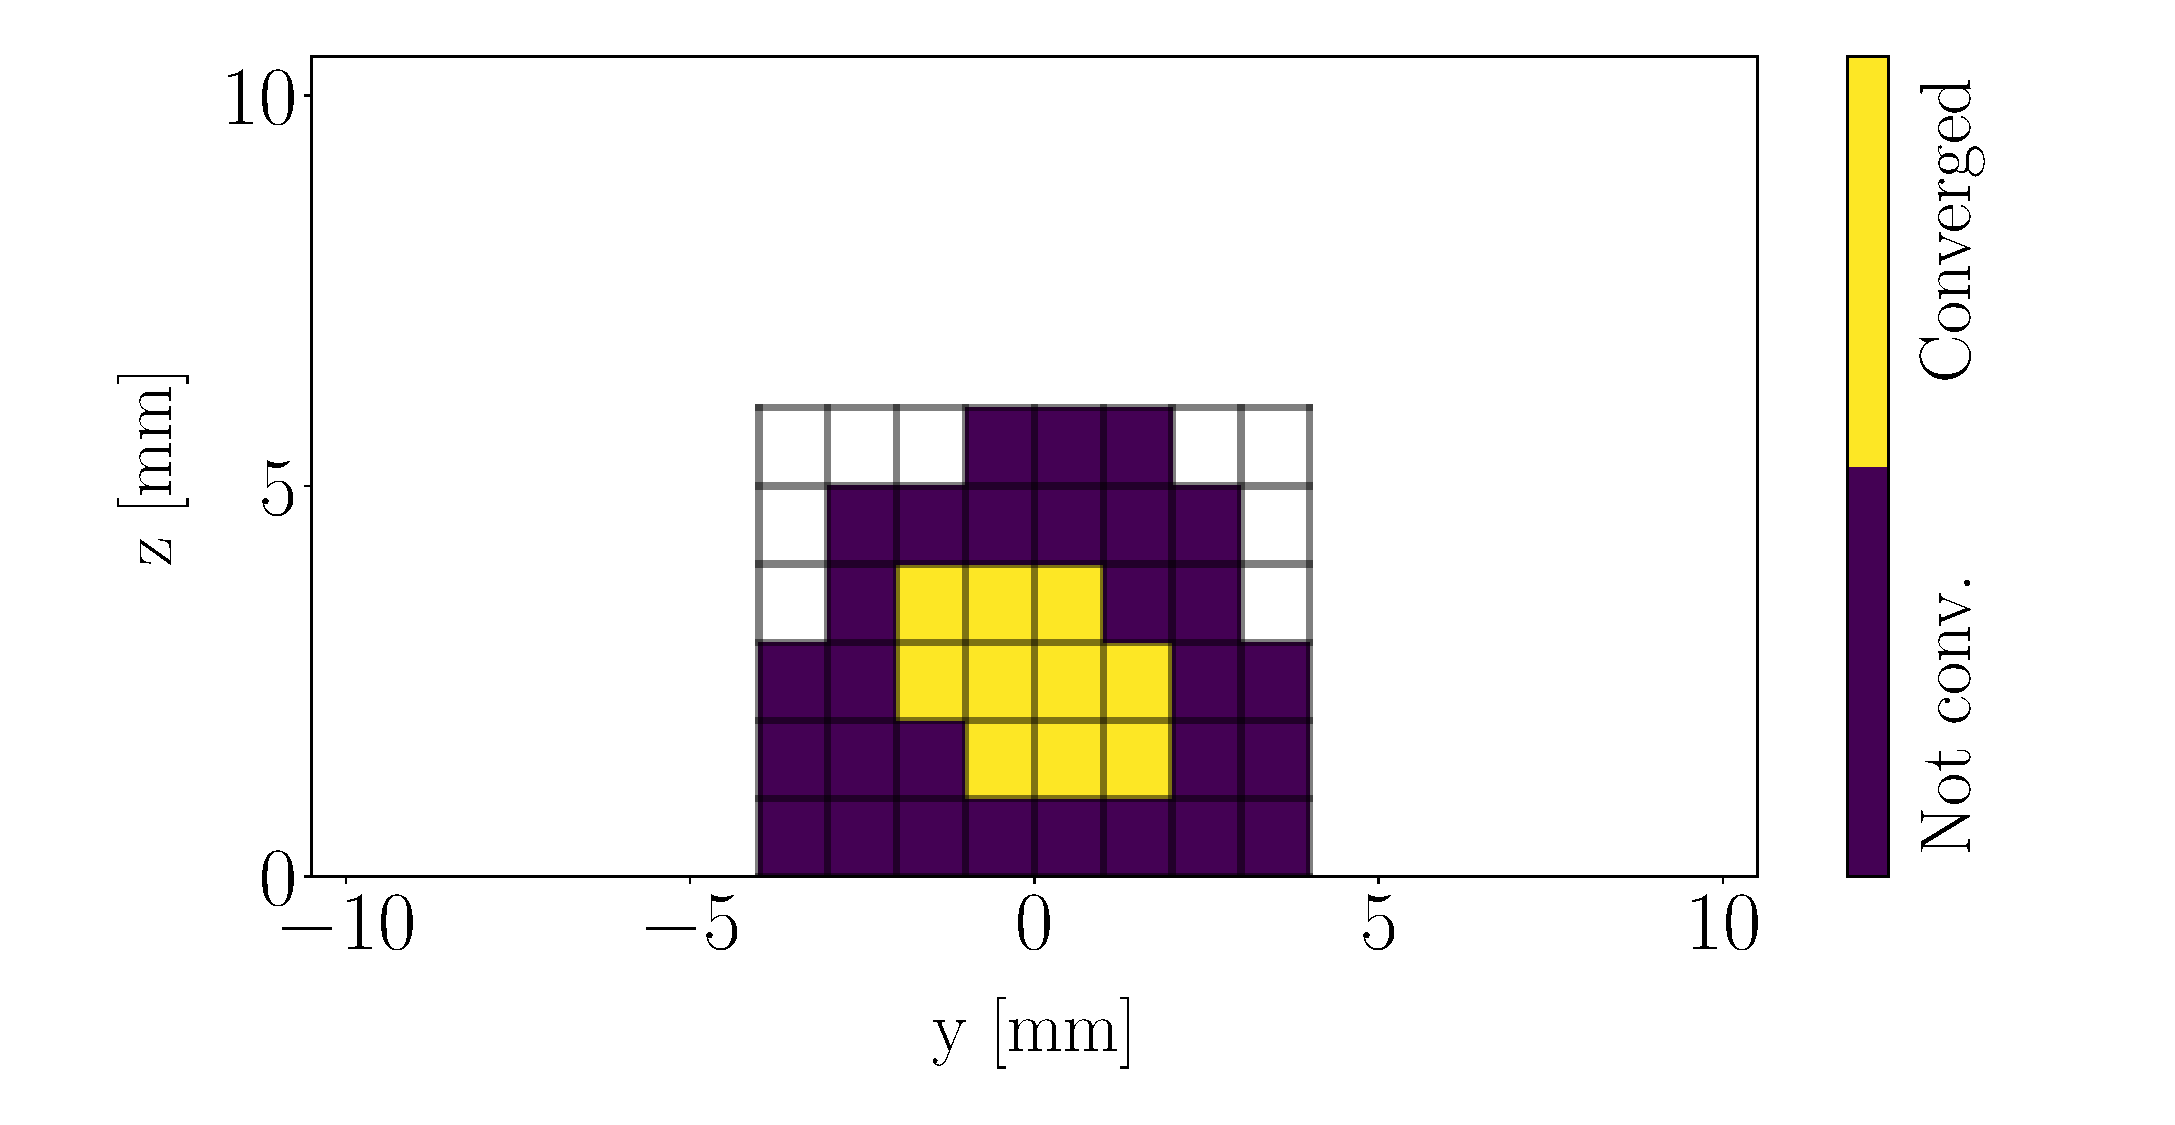
\includegraphics[scale=\scaleSLIJICF]{./part2_developments/figures_ch5_resolved_JICF/injectors_SLI/uG100_dx20_x05_convergence_map}
   %\caption{Case UG100\_DX10: crossflow planes}
   %\label{} 
\end{subfigure}

\vskip\baselineskip

\begin{subfigure}[b]{0.3\textwidth}
	\centering
   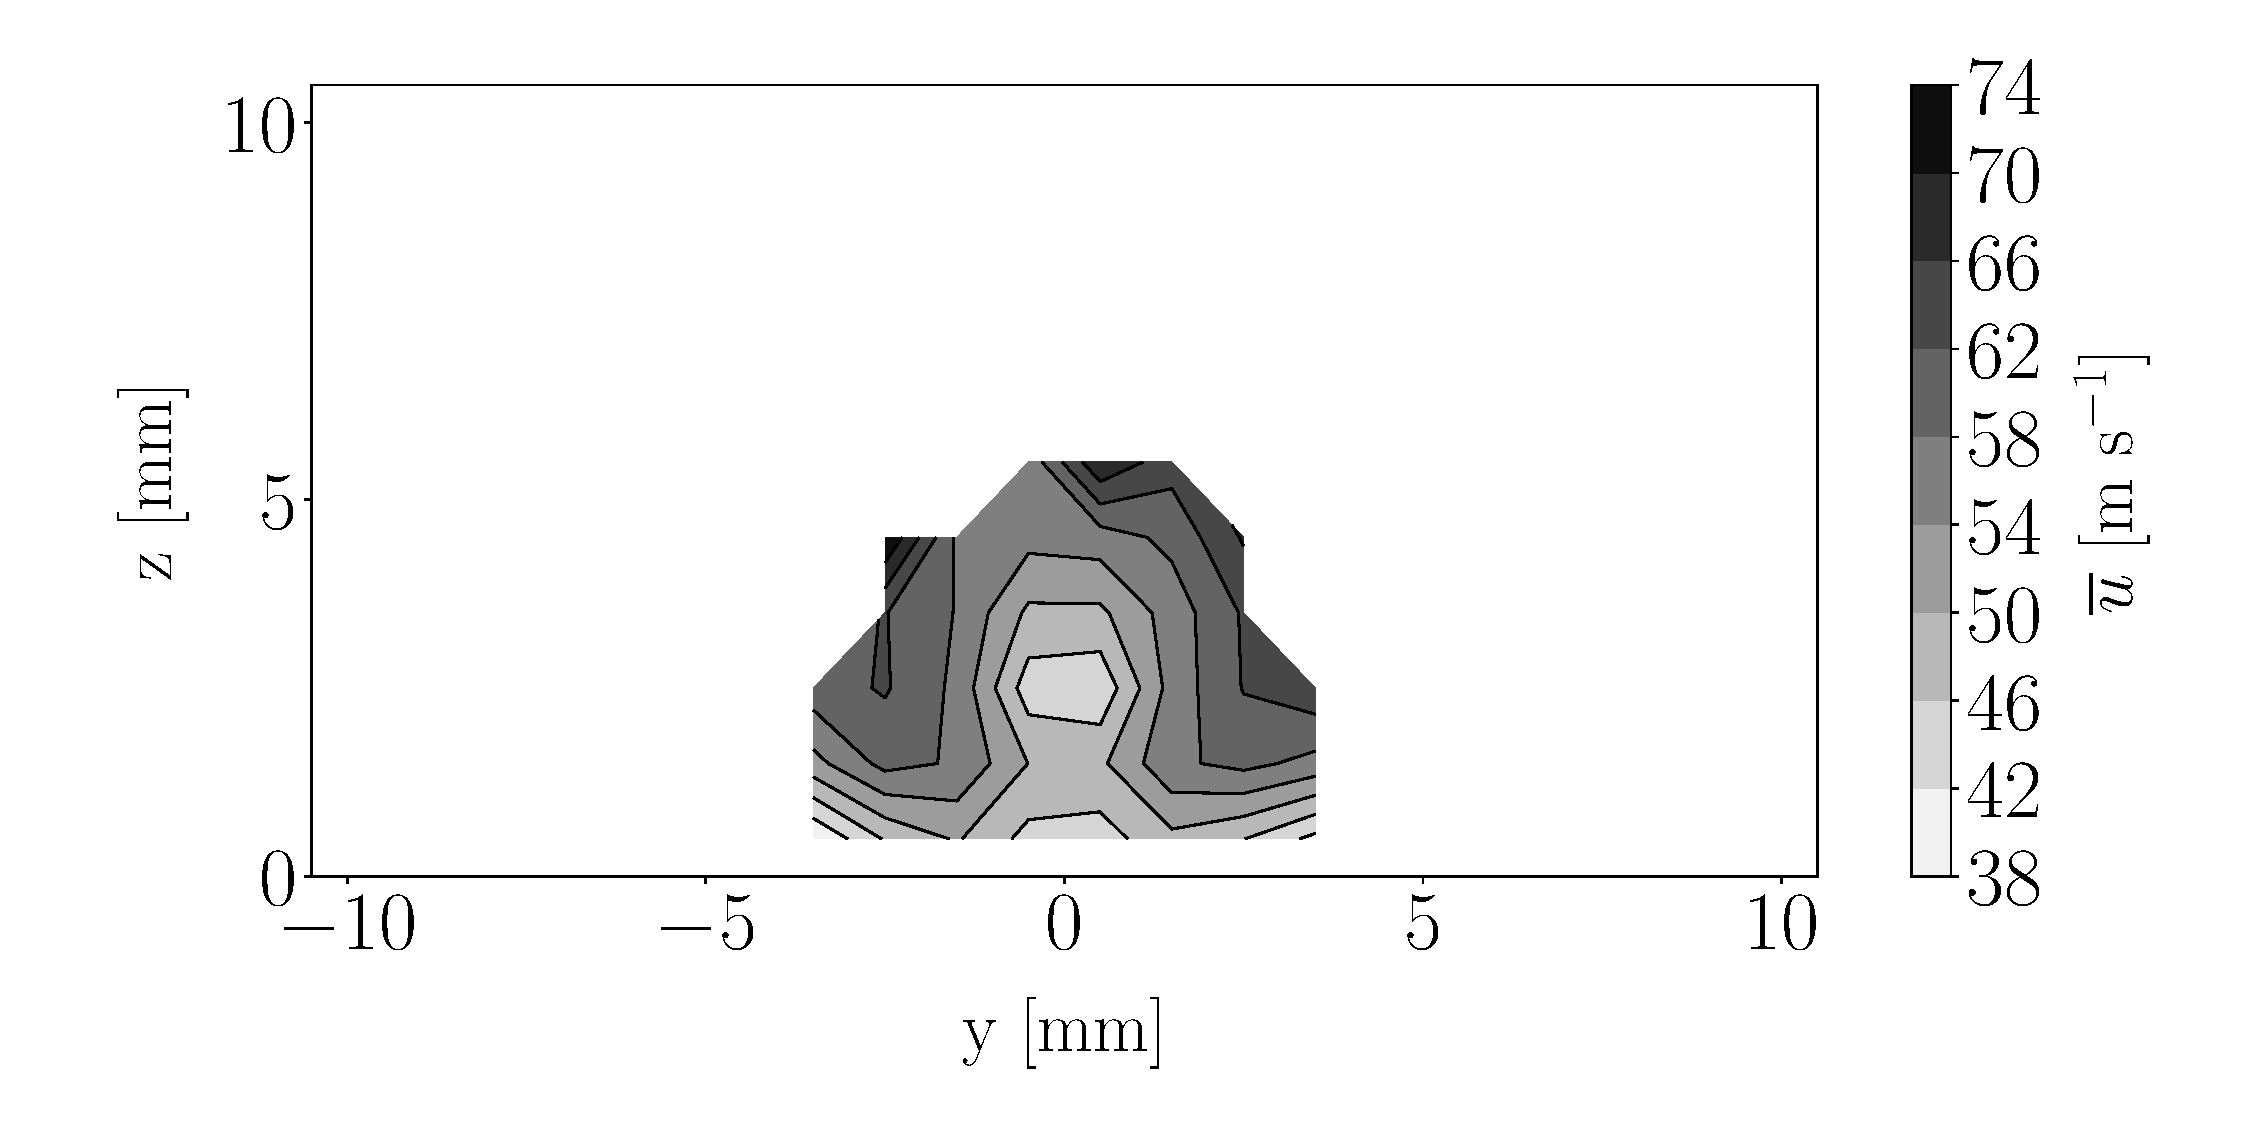
\includegraphics[scale=\scaleSLIJICF]{./part2_developments/figures_ch5_resolved_JICF/injectors_SLI/uG100_dx20_x05_ux_mean_map}
   %\caption{Case UG100\_DX20: crossflow planes}
   %\label{} 
\end{subfigure}
   \hspace{0.17in}
\begin{subfigure}[b]{0.3\textwidth}
	\centering
   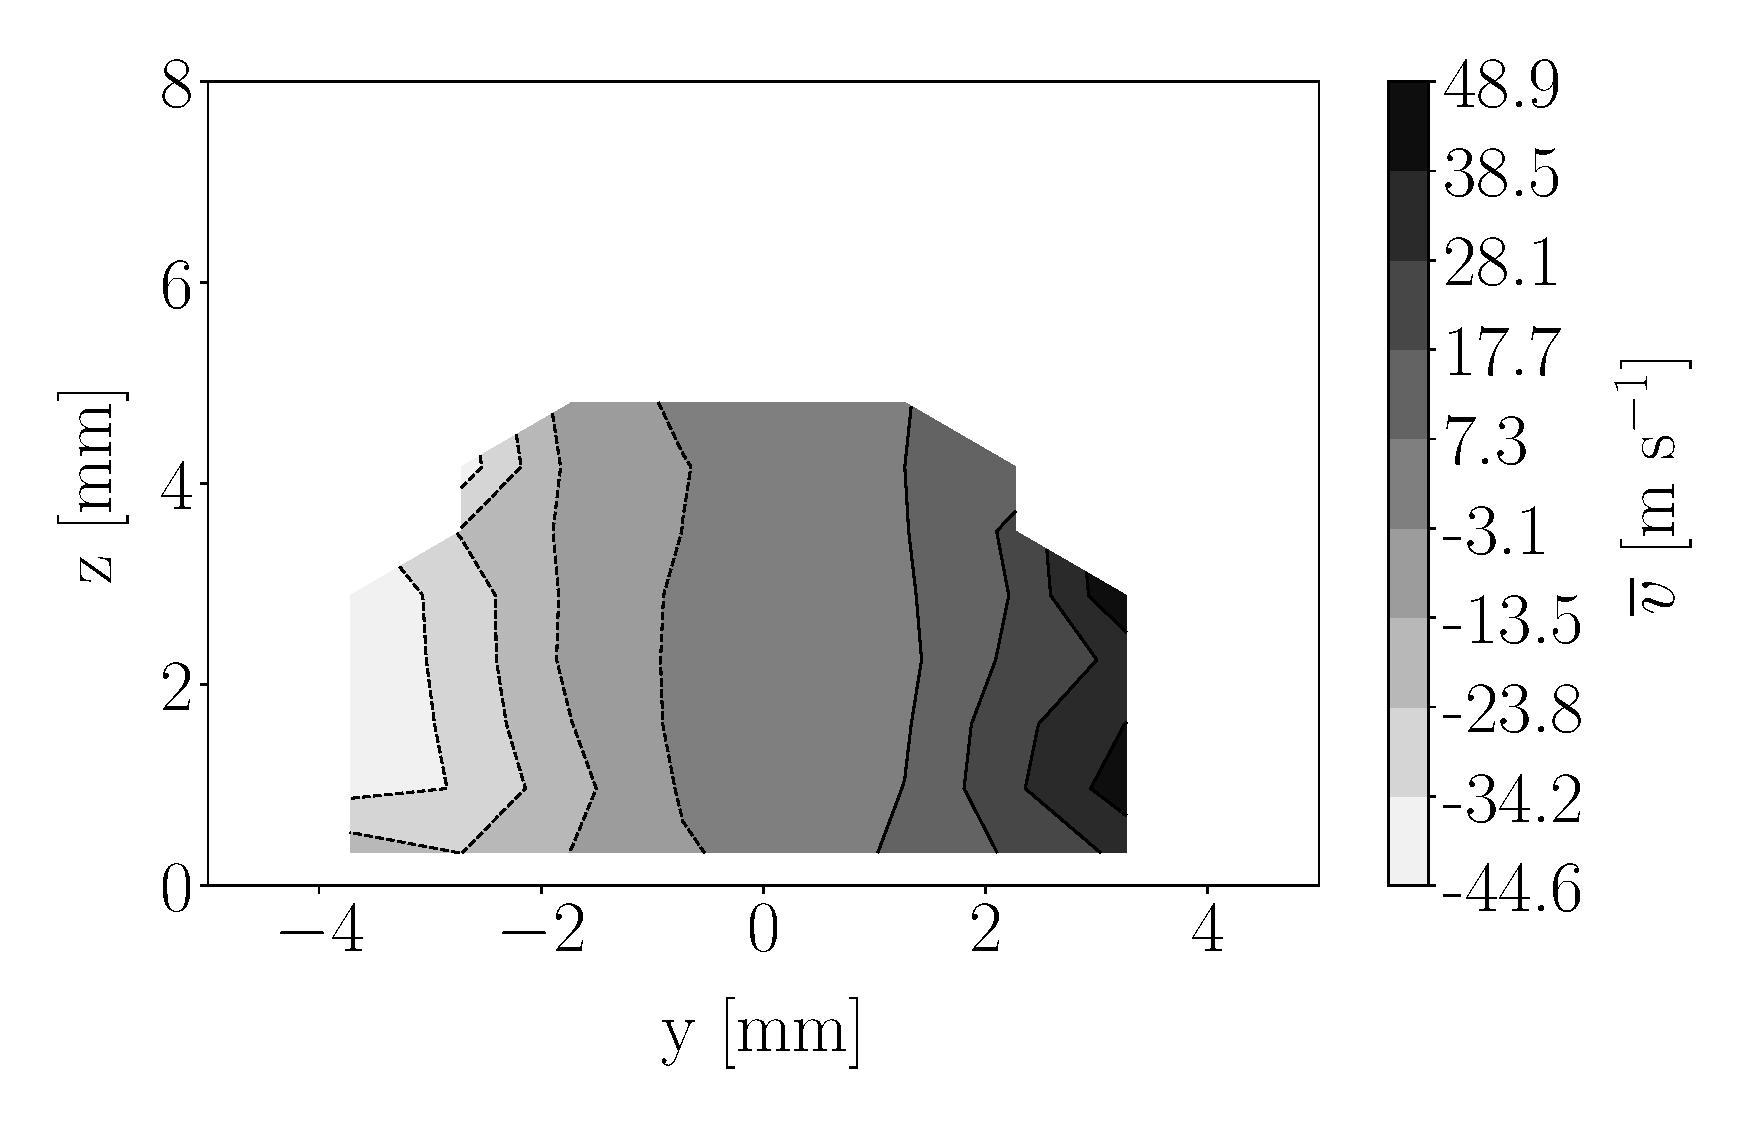
\includegraphics[scale=\scaleSLIJICF]{./part2_developments/figures_ch5_resolved_JICF/injectors_SLI/uG100_dx20_x05_uy_mean_map}
   %\caption{Case UG100\_DX20: filming planes}
   %\label{}
\end{subfigure}
   \hspace{0.17in}
\begin{subfigure}[b]{0.3\textwidth}
	\centering
   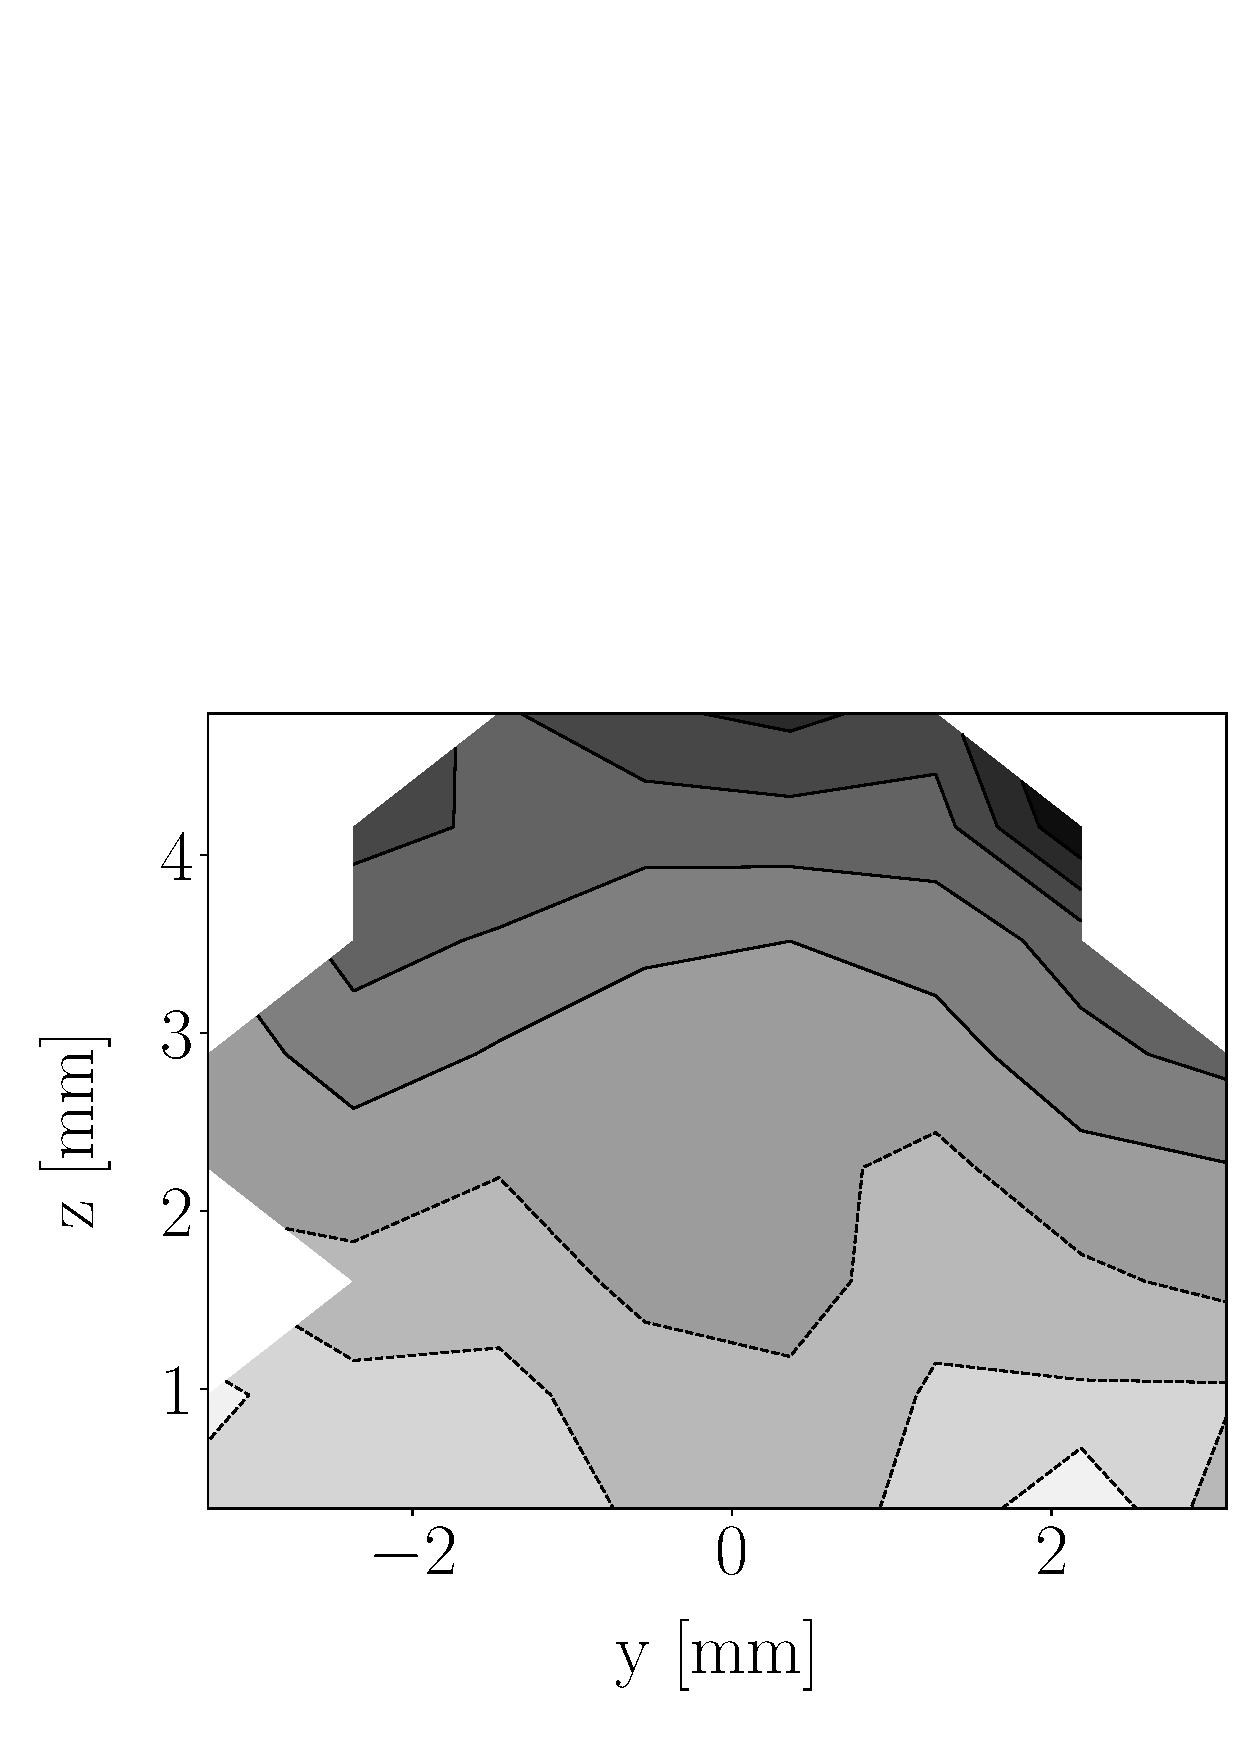
\includegraphics[scale=\scaleSLIJICF]{./part2_developments/figures_ch5_resolved_JICF/injectors_SLI/uG100_dx20_x05_uz_mean_map}
   %\caption{Case UG100\_DX10: crossflow planes}
   %\label{} 
\end{subfigure}
\caption{Spray states at x = 5 mm for case UG100\_DX20}
\label{fig:injectors_sli_uG100_dx20_x05}
\end{figure}


%%%%%%%%%%%%%%%% UG100_DX10, x = 10 mm


\begin{figure}[h!]
\centering
\begin{subfigure}[b]{0.3\textwidth}
	\centering
   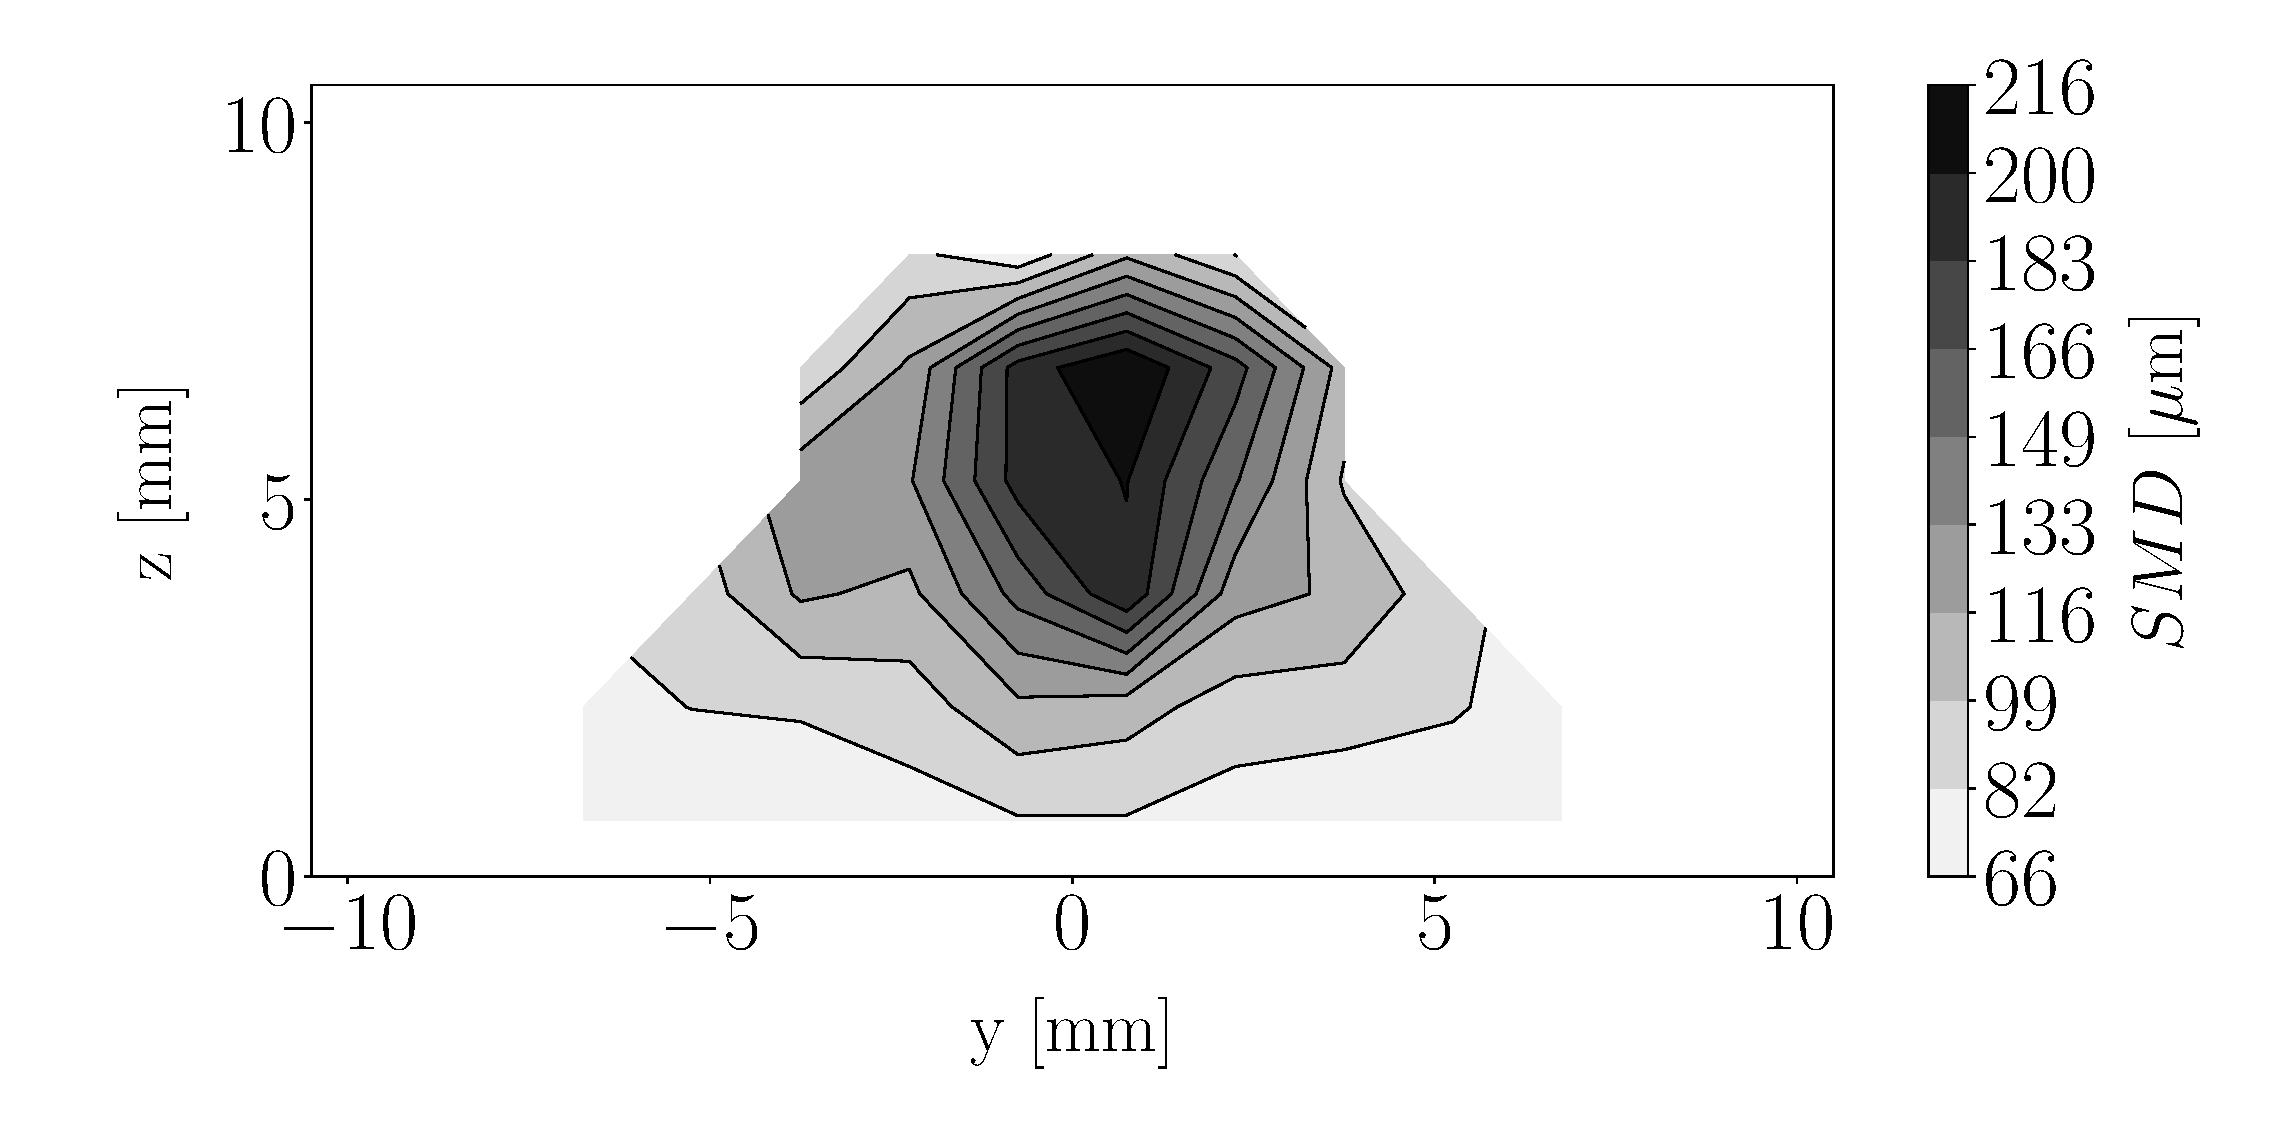
\includegraphics[scale=\scaleSLIJICF]{./part2_developments/figures_ch5_resolved_JICF/injectors_SLI/uG100_dx20_x10_SMD_map}
   %\caption{Case UG100\_DX20: crossflow planes}
   %\label{} 
\end{subfigure}
   \hspace{0.17in}
\begin{subfigure}[b]{0.3\textwidth}
	\centering
   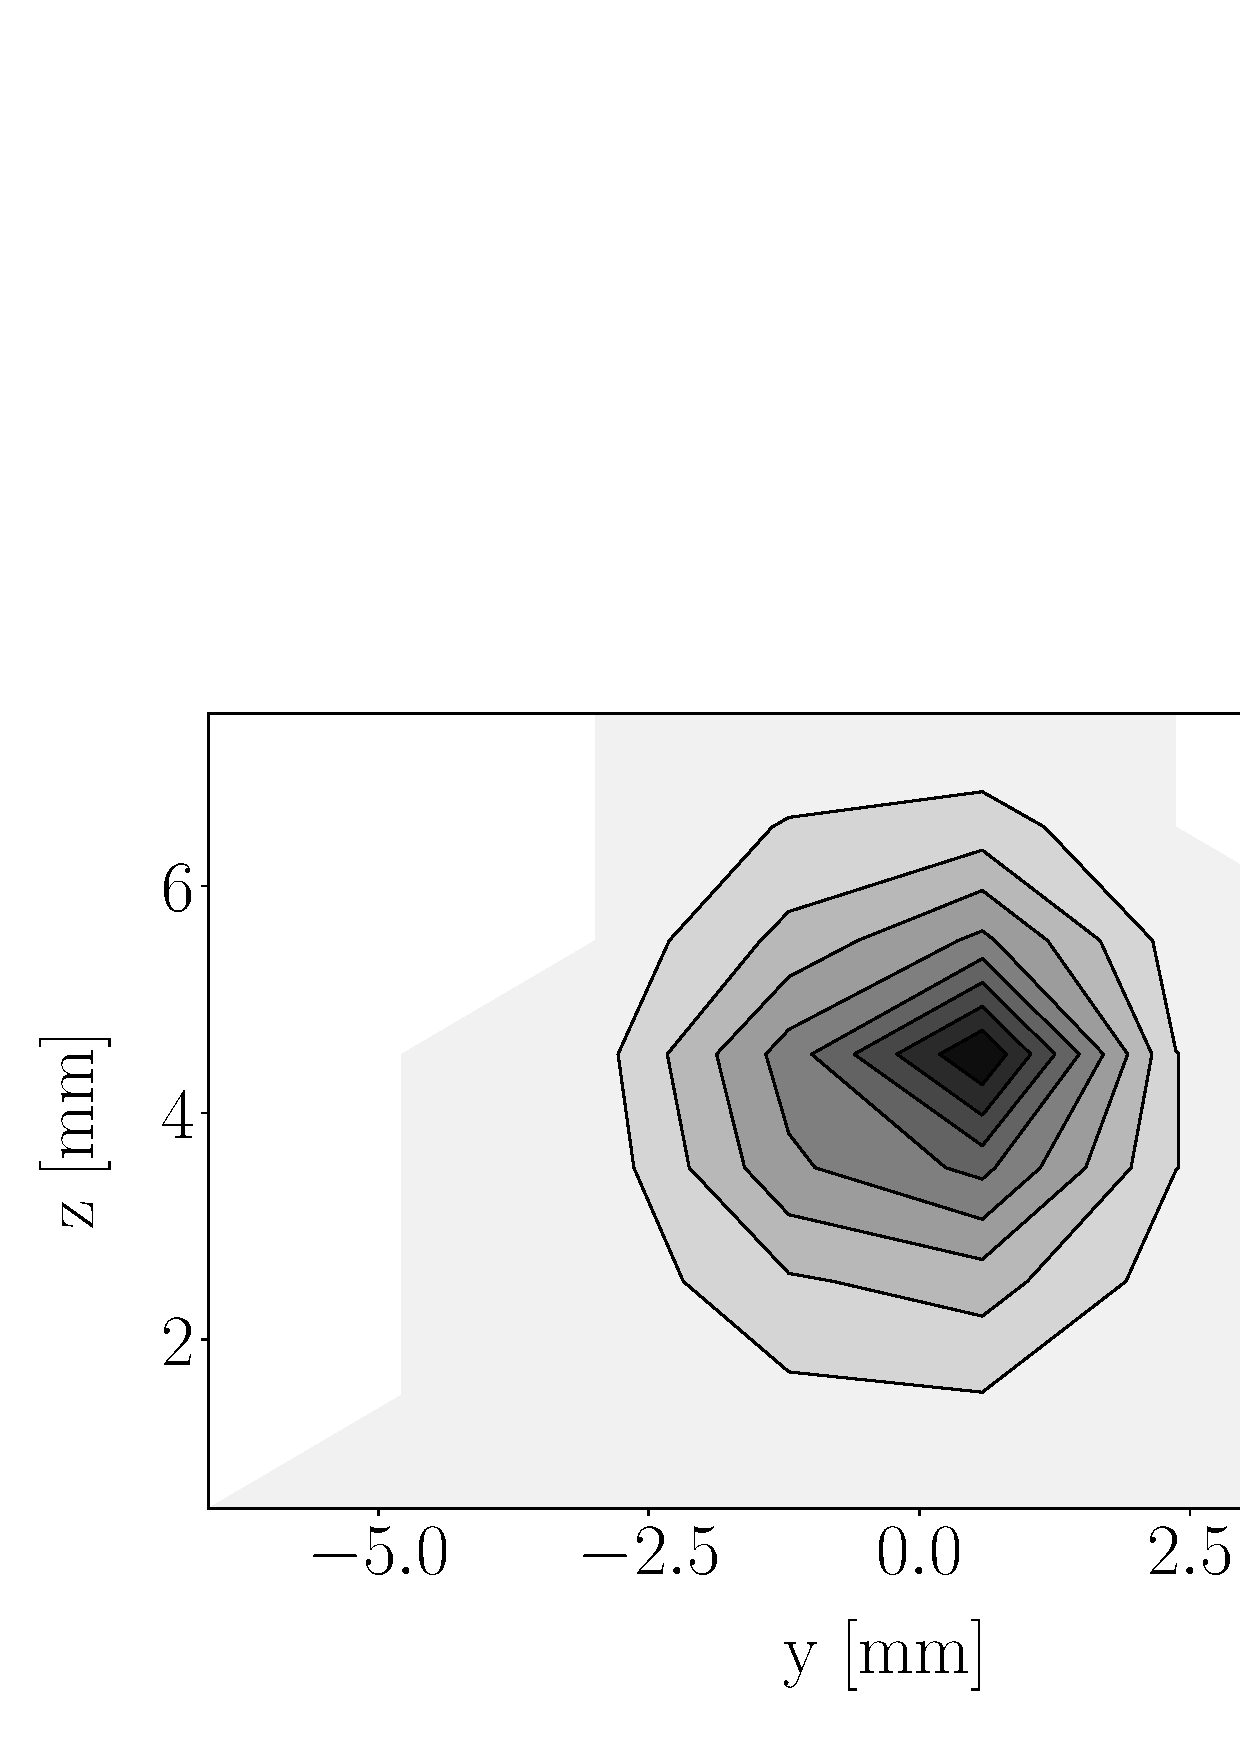
\includegraphics[scale=\scaleSLIJICF]{./part2_developments/figures_ch5_resolved_JICF/injectors_SLI/uG100_dx20_x10_volume_flux_map}
   %\caption{Case UG100\_DX20: filming planes}
   %\label{}
\end{subfigure}
   \hspace{0.17in}
\begin{subfigure}[b]{0.3\textwidth}
	\centering
   \includegraphics[scale=\scaleSLIJICF]{./part2_developments/figures_ch5_resolved_JICF/injectors_SLI/uG100_dx20_x10_convergence_map}
   %\caption{Case UG100\_DX10: crossflow planes}
   %\label{} 
\end{subfigure}

\vskip\baselineskip

\begin{subfigure}[b]{0.3\textwidth}
	\centering
   \includegraphics[scale=\scaleSLIJICF]{./part2_developments/figures_ch5_resolved_JICF/injectors_SLI/uG100_dx20_x10_ux_mean_map}
   %\caption{Case UG100\_DX20: crossflow planes}
   %\label{} 
\end{subfigure}
   \hspace{0.17in}
\begin{subfigure}[b]{0.3\textwidth}
	\centering
   \includegraphics[scale=\scaleSLIJICF]{./part2_developments/figures_ch5_resolved_JICF/injectors_SLI/uG100_dx20_x10_uy_mean_map}
   %\caption{Case UG100\_DX20: filming planes}
   %\label{}
\end{subfigure}
   \hspace{0.17in}
\begin{subfigure}[b]{0.3\textwidth}
	\centering
   \includegraphics[scale=\scaleSLIJICF]{./part2_developments/figures_ch5_resolved_JICF/injectors_SLI/uG100_dx20_x10_uz_mean_map}
   %\caption{Case UG100\_DX10: crossflow planes}
   %\label{} 
\end{subfigure}
\caption{Spray states at x = 10 mm for case UG100\_DX20}
\label{fig:injectors_sli_uG100_dx20_x10}
\end{figure}


%%%%%%%%%%%%%%%% UG100_DX10, x = 15 mm


\begin{figure}[h!]
\centering
\begin{subfigure}[b]{0.3\textwidth}
	\centering
   \includegraphics[scale=\scaleSLIJICF]{./part2_developments/figures_ch5_resolved_JICF/injectors_SLI/uG100_dx20_x15_SMD_map}
   %\caption{Case UG100\_DX20: crossflow planes}
   %\label{} 
\end{subfigure}
   \hspace{0.17in}
\begin{subfigure}[b]{0.3\textwidth}
	\centering
   \includegraphics[scale=\scaleSLIJICF]{./part2_developments/figures_ch5_resolved_JICF/injectors_SLI/uG100_dx20_x15_volume_flux_map}
   %\caption{Case UG100\_DX20: filming planes}
   %\label{}
\end{subfigure}
   \hspace{0.17in}
\begin{subfigure}[b]{0.3\textwidth}
	\centering
   \includegraphics[scale=\scaleSLIJICF]{./part2_developments/figures_ch5_resolved_JICF/injectors_SLI/uG100_dx20_x15_convergence_map}
   %\caption{Case UG100\_DX10: crossflow planes}
   %\label{} 
\end{subfigure}

\vskip\baselineskip

\begin{subfigure}[b]{0.3\textwidth}
	\centering
   \includegraphics[scale=\scaleSLIJICF]{./part2_developments/figures_ch5_resolved_JICF/injectors_SLI/uG100_dx20_x15_ux_mean_map}
   %\caption{Case UG100\_DX20: crossflow planes}
   %\label{} 
\end{subfigure}
   \hspace{0.17in}
\begin{subfigure}[b]{0.3\textwidth}
	\centering
   \includegraphics[scale=\scaleSLIJICF]{./part2_developments/figures_ch5_resolved_JICF/injectors_SLI/uG100_dx20_x15_uy_mean_map}
   %\caption{Case UG100\_DX20: filming planes}
   %\label{}
\end{subfigure}
   \hspace{0.17in}
\begin{subfigure}[b]{0.3\textwidth}
	\centering
   \includegraphics[scale=\scaleSLIJICF]{./part2_developments/figures_ch5_resolved_JICF/injectors_SLI/uG100_dx20_x15_uz_mean_map}
   %\caption{Case UG100\_DX10: crossflow planes}
   %\label{} 
\end{subfigure}
\caption{Spray states at x = 15 mm for case UG100\_DX20}
\label{fig:injectors_sli_uG100_dx20_x15}
\end{figure}

%\subsection{Feeding the models (??)}
%Find a more attractive name


\clearpage

\subsubsection*{Case UG100\_DX20\_NT}



%%%%%%%%%%%%%%%% UG100_DX20_NT, x = 5 mm


\begin{figure}[h!]
\centering
\begin{subfigure}[b]{0.3\textwidth}
	\centering
   \includegraphics[scale=\scaleSLIJICF]{./part2_developments/figures_ch5_resolved_JICF/injectors_SLI/uG100_dx20_x05_NT_SMD_map}
   %\caption{Case UG100\_DX20: crossflow planes}
   %\label{} 
\end{subfigure}
   \hspace{0.17in}
\begin{subfigure}[b]{0.3\textwidth}
	\centering
   \includegraphics[scale=\scaleSLIJICF]{./part2_developments/figures_ch5_resolved_JICF/injectors_SLI/uG100_dx20_x05_NT_volume_flux_map}
   %\caption{Case UG100\_DX20: filming planes}
   %\label{}
\end{subfigure}
   \hspace{0.17in}
\begin{subfigure}[b]{0.3\textwidth}
	\centering
   \includegraphics[scale=\scaleSLIJICF]{./part2_developments/figures_ch5_resolved_JICF/injectors_SLI/uG100_dx20_x05_NT_convergence_map}
   %\caption{Case UG100\_DX10: crossflow planes}
   %\label{} 
\end{subfigure}

\vskip\baselineskip

\begin{subfigure}[b]{0.3\textwidth}
	\centering
   \includegraphics[scale=\scaleSLIJICF]{./part2_developments/figures_ch5_resolved_JICF/injectors_SLI/uG100_dx20_x05_NT_ux_mean_map}
   %\caption{Case UG100\_DX20: crossflow planes}
   %\label{} 
\end{subfigure}
   \hspace{0.17in}
\begin{subfigure}[b]{0.3\textwidth}
	\centering
   \includegraphics[scale=\scaleSLIJICF]{./part2_developments/figures_ch5_resolved_JICF/injectors_SLI/uG100_dx20_x05_NT_uy_mean_map}
   %\caption{Case UG100\_DX20: filming planes}
   %\label{}
\end{subfigure}
   \hspace{0.17in}
\begin{subfigure}[b]{0.3\textwidth}
	\centering
   \includegraphics[scale=\scaleSLIJICF]{./part2_developments/figures_ch5_resolved_JICF/injectors_SLI/uG100_dx20_x05_NT_uz_mean_map}
   %\caption{Case UG100\_DX10: crossflow planes}
   %\label{} 
\end{subfigure}
\caption{Spray states at x = 5 mm for case UG100\_DX20\_NT}
\label{fig:injectors_sli_uG100_dx20_x05_NT}
\end{figure}


%%%%%%%%%%%%%%%% UG100_DX20_NT, x = 10 mm

\begin{figure}[h!]
\centering
\begin{subfigure}[b]{0.3\textwidth}
	\centering
   \includegraphics[scale=\scaleSLIJICF]{./part2_developments/figures_ch5_resolved_JICF/injectors_SLI/uG100_dx20_x10_NT_SMD_map}
   %\caption{Case UG100\_DX20: crossflow planes}
   %\label{} 
\end{subfigure}
   \hspace{0.17in}
\begin{subfigure}[b]{0.3\textwidth}
	\centering
   \includegraphics[scale=\scaleSLIJICF]{./part2_developments/figures_ch5_resolved_JICF/injectors_SLI/uG100_dx20_x10_NT_volume_flux_map}
   %\caption{Case UG100\_DX20: filming planes}
   %\label{}
\end{subfigure}
   \hspace{0.17in}
\begin{subfigure}[b]{0.3\textwidth}
	\centering
   \includegraphics[scale=\scaleSLIJICF]{./part2_developments/figures_ch5_resolved_JICF/injectors_SLI/uG100_dx20_x10_NT_convergence_map}
   %\caption{Case UG100\_DX10: crossflow planes}
   %\label{} 
\end{subfigure}

\vskip\baselineskip

\begin{subfigure}[b]{0.3\textwidth}
	\centering
   \includegraphics[scale=\scaleSLIJICF]{./part2_developments/figures_ch5_resolved_JICF/injectors_SLI/uG100_dx20_x10_NT_ux_mean_map}
   %\caption{Case UG100\_DX20: crossflow planes}
   %\label{} 
\end{subfigure}
   \hspace{0.17in}
\begin{subfigure}[b]{0.3\textwidth}
	\centering
   \includegraphics[scale=\scaleSLIJICF]{./part2_developments/figures_ch5_resolved_JICF/injectors_SLI/uG100_dx20_x10_NT_uy_mean_map}
   %\caption{Case UG100\_DX20: filming planes}
   %\label{}
\end{subfigure}
   \hspace{0.17in}
\begin{subfigure}[b]{0.3\textwidth}
	\centering
   \includegraphics[scale=\scaleSLIJICF]{./part2_developments/figures_ch5_resolved_JICF/injectors_SLI/uG100_dx20_x10_NT_uz_mean_map}
   %\caption{Case UG100\_DX10: crossflow planes}
   %\label{} 
\end{subfigure}
\caption{Spray states at x = 10 mm for case UG100\_DX20\_NT}
\label{fig:injectors_sli_uG100_dx20_x10_NT}
\end{figure}

\clearpage


\subsubsection*{Inhomogeneity of sprays}
%\label{subsec:SPS_inhomogeneity_sprays}

The resulting spray from a JICF is highly polydisperse and velocity-inhomogeneous, as shown by the previous spatial maps. The proposed SLI approach allows to directly account for these spray characteristics by prescribing spatially discretized statistics in dispersed-phase simulations. This spatial discretization procedure can also be seen as dividing the global in-plane accumulated spray into several individual sprays, each one contained in every discretization probe. Then, each probe will represent a monodisperse spray by accounting only for mean statistics on the diameters (SMD) and velocities. However, the polydispersity and inhomogeneity of each probe's spray should also be taken into account when performing injection.

In order to illustrate this inhomogeneity within the local probes, Figure \ref{fig:injectors_SLI_extra_UG100_DX10_x05} shows the maps of volume flux, arithmetic mean and volume-weighted (VW) velocities at $x = 5$ mm for case UG100\_DX10. The probe containing the largest flux is highlighted in blue. The velocity maps show a different spatial distribution of the velocity when considering volume-weighted statistics or not: the VW velocity displays lower magnitudes in all the plane, since actually more importance is given to the large droplets which are slower than the smaller ones. Exceptions are observed where fluxes are the lowest, since the amount of droplets is scarce and the arithmetic mean and VW velocities get closer. The spray at maximum flux probe (i.e. the one with more sampled droplets) is further analyzed by plotting the droplet size $D$ and axial velocity $u$ histograms, as well as the scatterplot $D - u$, in Figure \ref{fig:injectors_extra_velocities_interesting}. In the size histogram the SMD is highlighted: if only the SMD is injected in the dispersed-phase simulations, a wide range of droplets sizes is actually neglected when prescribing the spray. Injection of a spray size distribution $f_0$ better representing the spray histogram will solvent this issue. The velocity histogram shows also a wide range of droplets velocities with respect to the mean ones: injecting a stochastic velocity given by a law such as the one from Eq. (\ref{eq:ch4_lagrangian_injection_velocity_with_mean_and_rms}), which also accounts for the RMS component will then consider the inhomogeneity of the droplets velocities. It is also noticeable the difference between arithmetic mean and VW velocities, 52 against 44 $\mathrm{m~s}^{-1}$ respectively: such differences at injection could greatly impact secondary atomization of droplets, which is highly dependent on the $We$ based on the relative velocity. These two influences, i.e polydispersity through $f_0$ and variations in injection velocity through Eq. (\ref{eq:ch4_lagrangian_injection_velocity_with_mean_and_rms}), will be investigated in the next chapter. Finally, it is interesting to highlight the dependence of droplets velocities on their sizes as shown in the scatterplot of Figure \ref{fig:injectors_extra_velocities_interesting} right. The arithmetic mean and VW velocities are represented by the horizontal black lines, while the $SMD$ is given by the vertical green line. The points where curves cross would represent the injection velocity and diameters if a monodisperse spray were to be injected: considering also the RMS through Eq. (\ref{eq:ch4_lagrangian_injection_velocity_with_mean_and_rms}) would enlarge the range of velocities to be injected, while also including a $f_0$ would enlarge the range of droplets sizes injected. The red line represents the mean velocity at diameter intervals when the $D$ axis is discretized into several bins (named sections). As shown, section mean velocities section can highly differ from the constant $\overline{u}$ of $\overline{u}_\mathrm{VW}$ ones. Further steps should consider the prescription of this $D - u$ conditioning in dispersed-phase simulations: this strategy is called sectional approach, and has been succesfully tested in lagrangian sprays \citepColor[vie_accounting_2013]. 



\begin{figure}[h!]
\centering
\begin{subfigure}[b]{0.3\textwidth}
	\centering
   \includegraphics[scale=0.225]{./part2_developments/figures_ch5_resolved_JICF/injectors_SLI_extra/uG100_dx10_x05_volume_flux_map}
   %\caption{Case UG100\_DX20: crossflow planes}
   %\label{} 
\end{subfigure}
   \hspace{0.17in}
\begin{subfigure}[b]{0.3\textwidth}
	\centering
   \includegraphics[scale=0.225]{./part2_developments/figures_ch5_resolved_JICF/injectors_SLI_extra/uG100_dx10_x05_ux_mean_map}
   %\caption{Case UG100\_DX20: filming planes}
   %\label{}
\end{subfigure}
   \hspace{0.17in}
\begin{subfigure}[b]{0.3\textwidth}
	\centering
   \includegraphics[scale=0.225]{./part2_developments/figures_ch5_resolved_JICF/injectors_SLI_extra/uG100_dx10_x05_ux_mean_VW_map}
   %\caption{Case UG100\_DX10: crossflow planes}
   %\label{} 
\end{subfigure}

\caption{Volume flux, arithmetic mean and volume-weighted axial velocities at $x = 5$ mm from case UG100\_DX10}
\label{fig:injectors_SLI_extra_UG100_DX10_x05}
\end{figure}

\clearpage


\begin{figure}[h!]
\centering
\begin{subfigure}[b]{0.3\textwidth}
	\centering
   \includegraphics[scale=0.24]{./part2_developments/figures_ch5_resolved_JICF/injectors_SLI_extra/uG100_dx10_x05_size_histogram}
   %\caption{Case UG100\_DX20: crossflow planes}
   %\label{} 
\end{subfigure}
   \hspace{0.17in}
\begin{subfigure}[b]{0.3\textwidth}
	\centering
   \includegraphics[scale=0.24]{./part2_developments/figures_ch5_resolved_JICF/injectors_SLI_extra/uG100_dx10_x05_vel_histogram}
   %\caption{Case UG100\_DX20: filming planes}
   %\label{}
\end{subfigure}
   \hspace{0.17in}
\begin{subfigure}[b]{0.3\textwidth}
	\centering
   \includegraphics[scale=0.24]{./part2_developments/figures_ch5_resolved_JICF/injectors_SLI_extra/uG100_dx10_x05_vel_scatter}
   %\caption{Case UG100\_DX10: crossflow planes}
   %\label{} 
\end{subfigure}

\caption[Histograms of droplets diameters $D$ (\textsl{left}) and axial velocity $u$ (\textsl{center}), and scatterplot $D - u$ (\textsl{right})]{Histograms of droplets diameters $D$ (\textsl{left}) and axial velocity $u$ (\textsl{center}), and scatterplot $D - u$ (\textsl{right}) for the spray contained within the highlighted probe of Figure \ref{fig:injectors_SLI_extra_UG100_DX10_x05}}
\label{fig:injectors_extra_velocities_interesting}
\end{figure}


\subsubsection*{On SLI convergenge time with resolution}



If obtaining a SLI with a coarse resolution takes a given particle's accumulation time to converge, it is reasonable to assume that a finer resolution also needs to simulate the same accumulation time. This, indeed, has shown not to be true: as illustrated by the convergence maps from Figures \ref{fig:injectors_sli_uG75_dx10_x05} to \ref{fig:injectors_sli_uG100_dx20_x10_NT}, SLIs obtained with the fine resolution present a greater number of converged local probes than the coarse ones. Even though the accumulation time is lower in the fine resolution simulations, finer liquid structures make injectors converge faster than in the coarse computations. Therefore, increasing the resolution decreases the accumulation time needed to yield a converged spray: producing a final SLI requires less computational resources than a priori thought. 

To illustrate the associated cost savings in computational time (named hereafter cost savings), let's consider the high Weber operating condition. The coarse simulation needs $t_\mathrm{ph} = 6.16$ ms to produce a converged SLI, while the fine one needs only $t_\mathrm{ph} = 0.78$ ms, i.e. 8 times less physical time. Therefore, if only the physical time is considered, it is a priori expected that a fine simulation should also run for $t_\mathrm{ph} = 6.16$ ms, increasing the cost from the coarse simulation by 8. Indeed, their actual computational costs are 1.25 and 4.66 million CPU hours for the coarse and fine simulations: the cost to obtain a more locally converged injector rises only 4 times. Figure \ref{fig:SLI_cost_convergence_savings} illustrates graphically this difference. The first and second columns show the absolute CPU hours from Figure \ref{fig:SLI_cost_convergence_all}. The third one shows the estimated cost to run a fine simulation as far as the coarse one, which would be of $t_\mathrm{CPU} = 36.7 \cdot 10^6$ hours. The cost savings are therefore estimated to be of $30.41 \cdot 10^6$ hours.

\begin{figure}[ht]
   \centering
   \includegraphics[scale=0.215]{./part2_developments/figures_ch5_resolved_JICF/SLI_cost_for_convergence/cost_savings_simulations}
   \caption{Cost savings in SLI development by refining grid resolution}
   \label{fig:SLI_cost_convergence_savings}
\end{figure}

 

